\chapter{Analysis}
\resetfootnote

\pagestyle{fancy}
\markboth{\bfseries \slshape Analysis}{}
\renewcommand{\sectionmark}[1]{\markright{\bfseries \slshape \thesection\ #1}{}}
\fancyhead[R]{\rightmark}
\fancyhead[L]{\leftmark}
\fancyfoot[R]{\sl Maurizio Ungaro}
\fancyfoot[L]{}

\section{Bins size}
\label{sec:binning}
The choice of bins size in the variables $W$, $Q^2$, $\cos\theta^*$, $\phi^*$
is illustrated in Fig.~\ref{fig:binning1} and Fig.~\ref{fig:binning2}.
The bin sizes were chosen to agree with previous and ongoing analyses.


$W$ was divided in $15$ bins from $1.1$ GeV to $1.4$ GeV in step of
$\Delta W = 0.02$ $GeV$. $\Delta Q^2$ is variable and such that $\Delta Q^2/Q^2\simeq 0.18$. 
The values are in table \ref{tab:binning}.

\begin{figure}[h]
 \begin{center}
  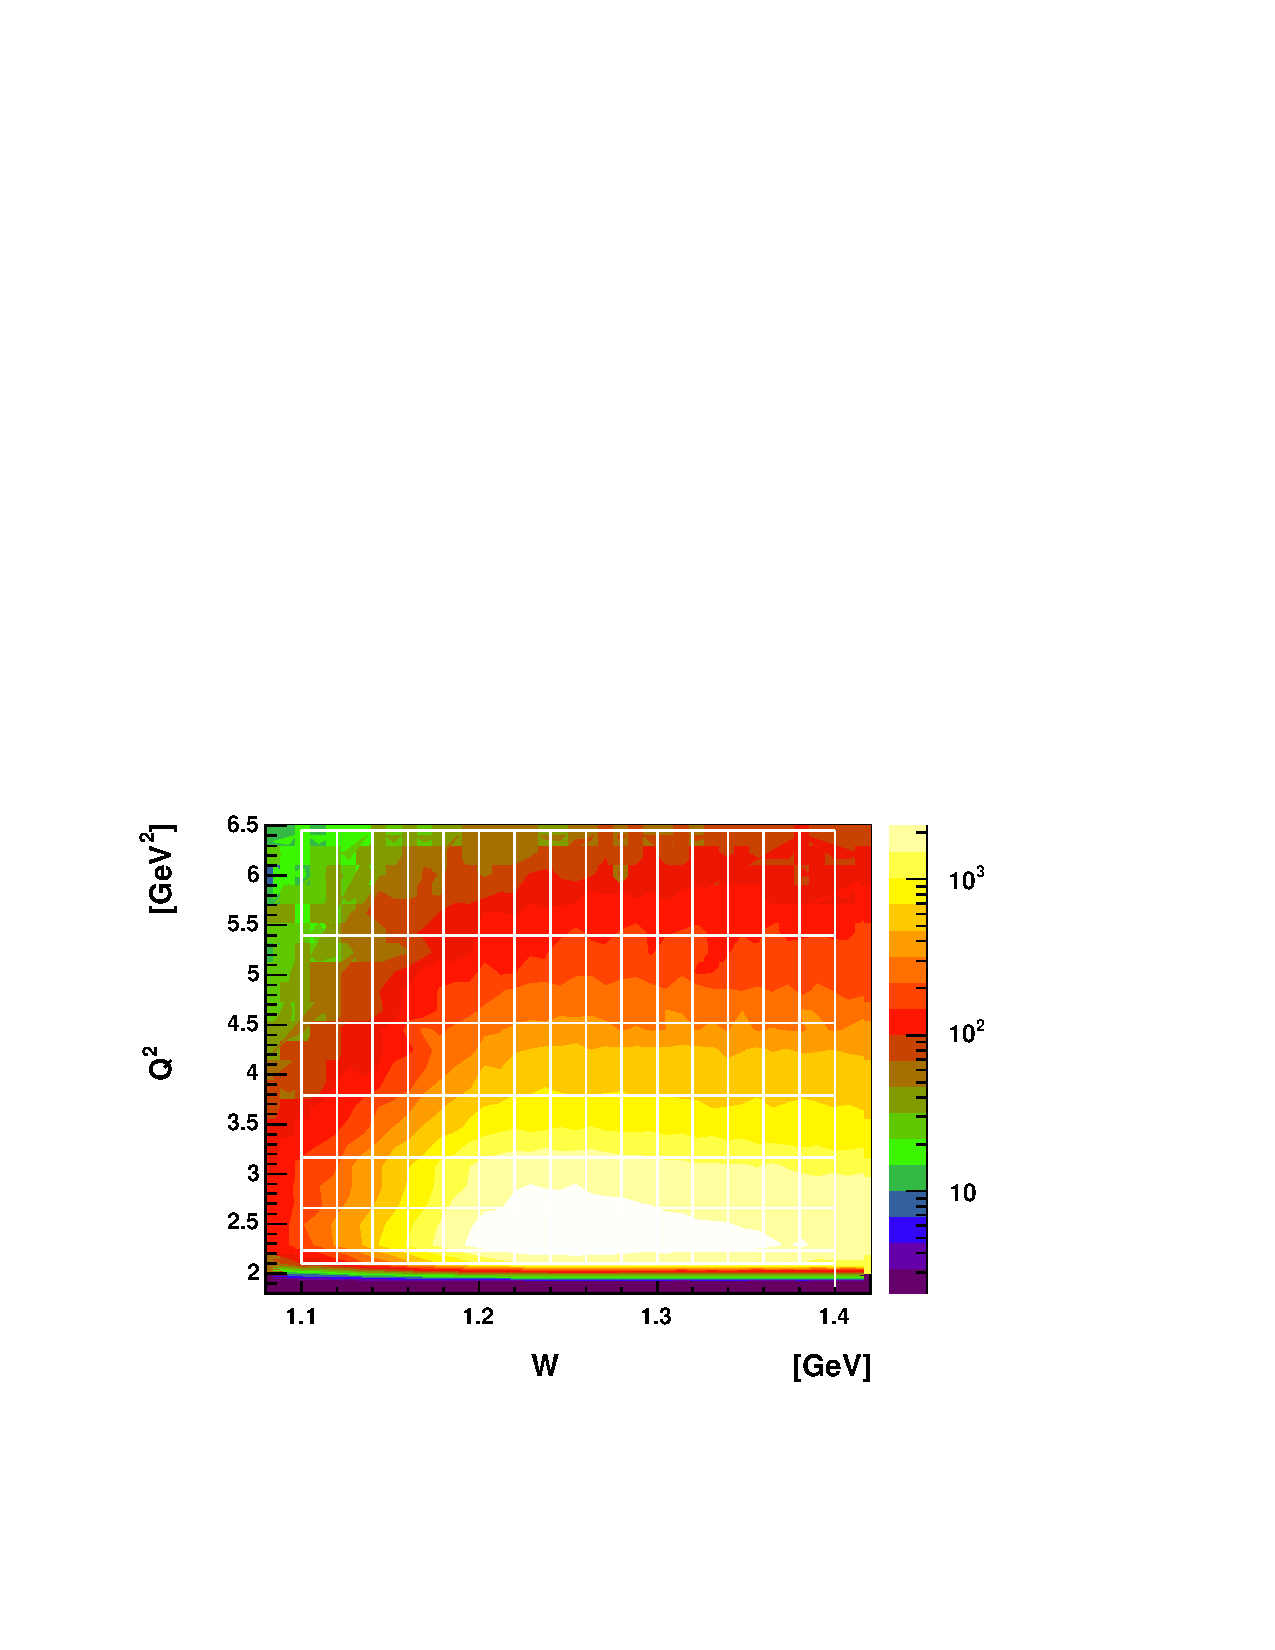
\includegraphics[width=12cm, bb=40 140 520 460]{analysis/img/binning1}
  \caption[$W$ and $Q^2$ binning for $\pi^0$ events]
          { $W$ and $Q^2$ binning for $\pi^0$ events (all angles). Notice the increasing $\Delta Q^2$ size with $Q^2$.}
 \label{fig:binning1}
  \end{center} 
\end{figure} 


\begin{table}[h]
 \begin{center}
  \begin{tabular}{|l|c|c|c|c|c|c|c|}
    \hline 
   $Q^2$        & 2.15  & 2.4  & 3.0  & 3.5  & 4.2  & 5.0  & 6.0 \\ 
    \hline  
   $Q^2_{min}$  & 2.10 & 2.23 & 2.66 & 3.17 & 3.79 & 4.52 & 5.40 \\
   \hline
   $Q^2_{max}$  & 2.23 & 2.66 & 3.17 & 3.79 & 4.52 & 5.40 & 6.45\\       
 \hline
  \end{tabular}
 \end{center} 
 \caption[The binning in $Q^2$]
         { The binning in $Q^2$.}
 \label{tab:binning}
\end{table}

The angular bins are taken as follows:
$\Delta \cos\theta^* = 0.2$ and $\Delta\phi^* = 30^0$ so that there are $10$ bins in  $\cos\theta^*$ and $12$ in $\phi^*$
as shown in  Fig.~\ref{fig:binning2}.
\begin{figure}[h]
 \begin{center}
  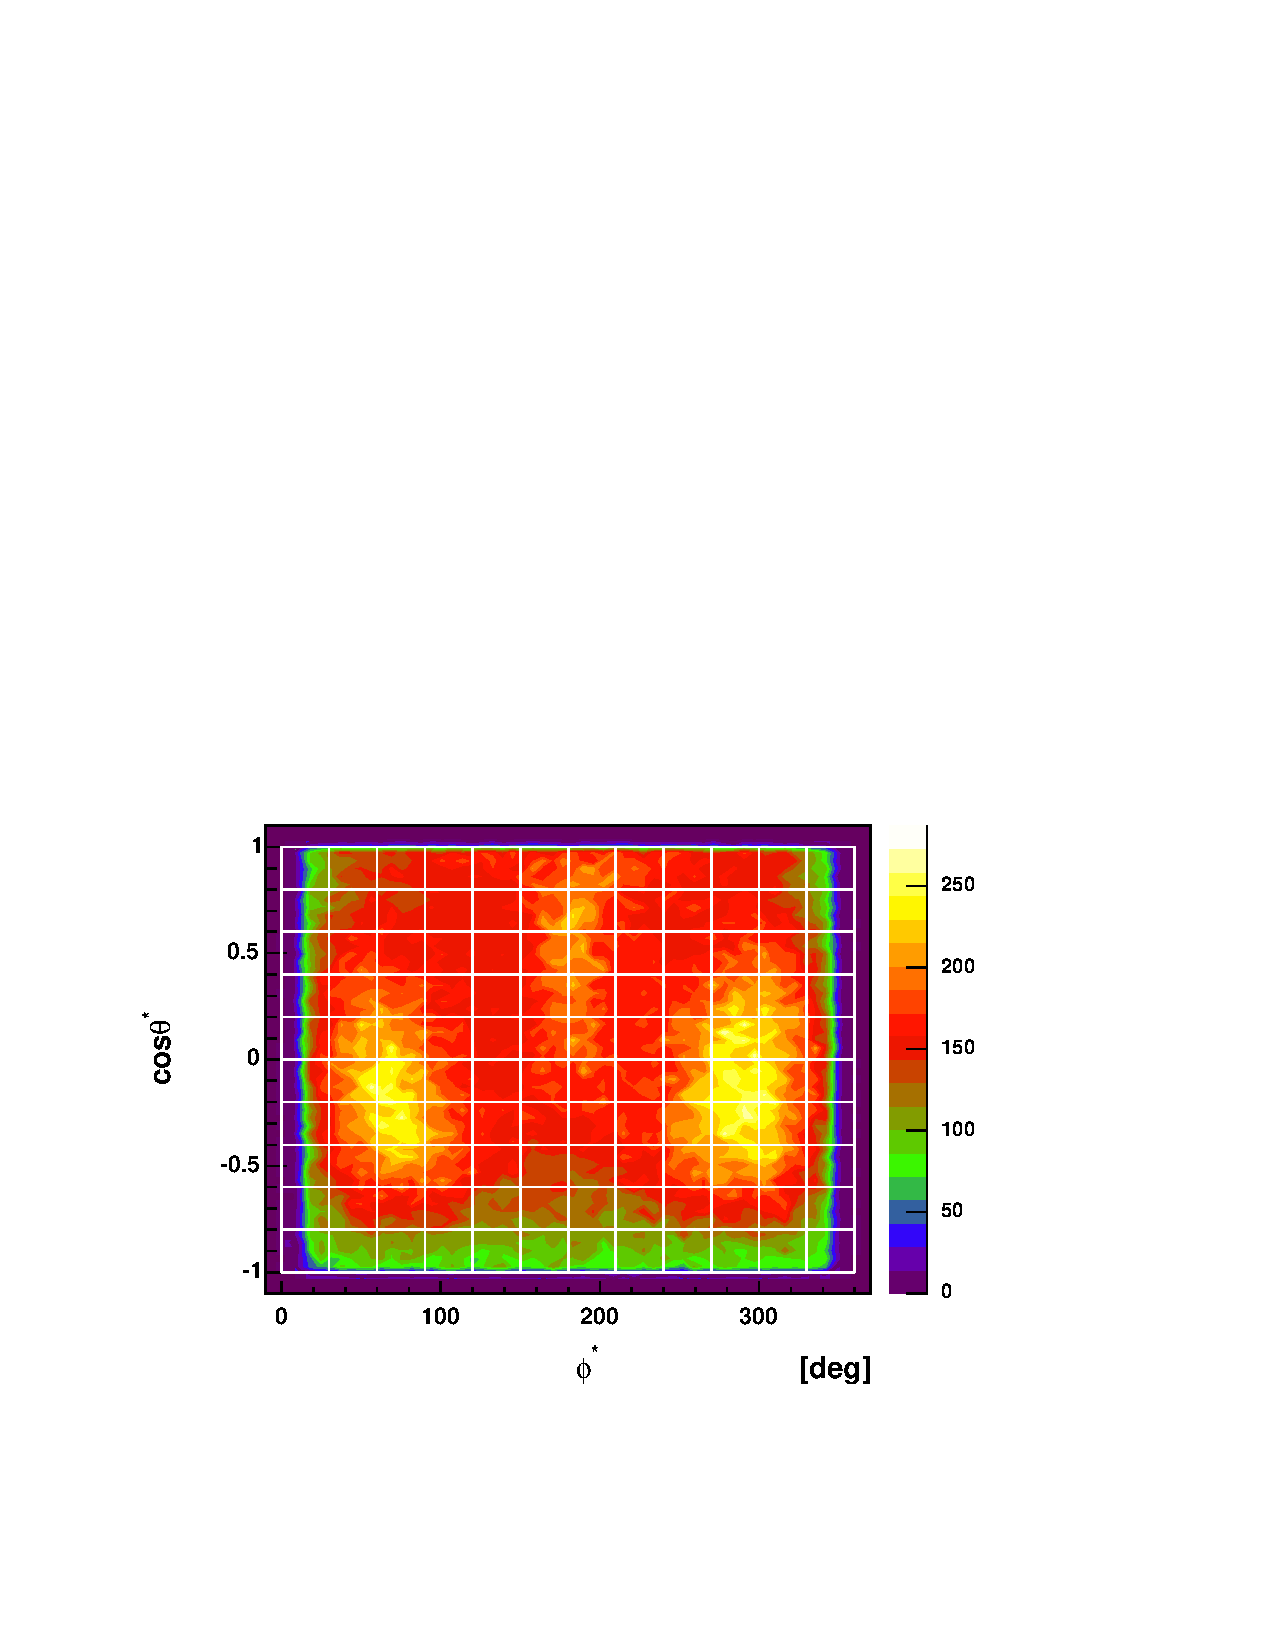
\includegraphics[width=12cm, bb=60 120 480 460]{analysis/img/binning2}
  \caption[$\cos\theta^*$ and $\phi^*$ binning for $\pi^0$ events]
          { $\cos\theta^*$ and $\phi^*$ binning for $\pi^0$ events (all $W$ and $Q^2$).}
 \label{fig:binning2}
\end{center} 
\end{figure}










\section{ Bin averaging correction}
When calculating the cross section, an average
in each bin occurs (see \F{fig:bin}. If the cross section distribution
is linear in all variables inside the bins then the value
at center corresponds to the value obtained. This is not the case 
in the more realistic situation when the data distribution
has some structure inside the bin. 

\begin{figure}[h]
\begin{center}
 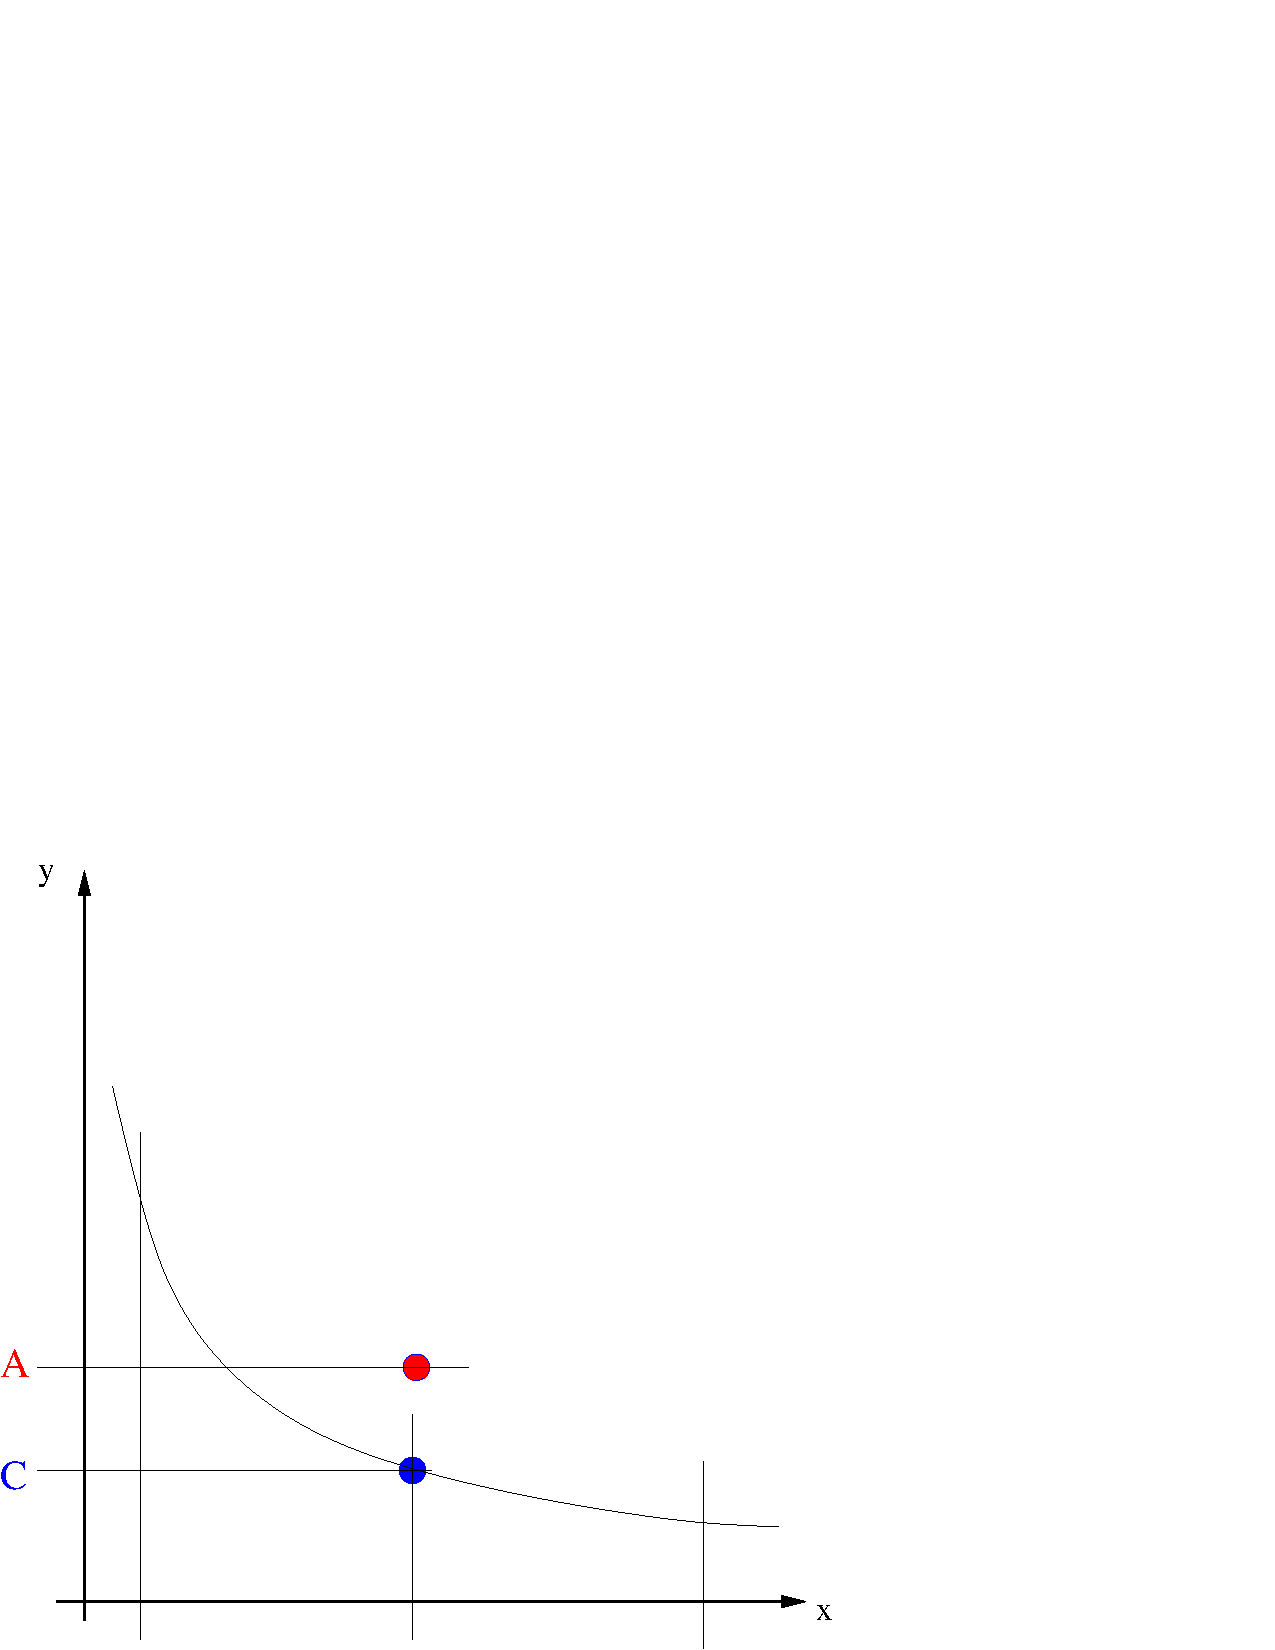
\includegraphics[width = 9cm, bb=-20 0 440 420]{analysis/img/bin}
  \caption[The bin correction]
          { The bin correction. $C$ is the value of the cross section at the center
	             of the bin, while $A$ is its average in that bin. The correction is $R=A/C$.}
 \label{fig:bin}
\end{center}
\end{figure}



To take in account this effect 
each bin was divided into subdivisions. The cross section
in each subdivision (using a model) was calculated to obtain the average $A$ in that 
whole bin. 
The value at the center of the bin $C$ was calculated as well. The resulting correction is
$$
 R = \Dfrac{C}{A}
$$





The model {\bf maid 2000 extended} \cite{bib:maid2000} is used to calculate the correction.
Each of the $15\times7\times12\times10 = 12600$ bins is divided into $15^4 = 50625$ subdivisions
($15$ for each of the variables $W$, $Q^2$, $\cos\theta$, $\phi$).
This gives a total of $\sim 600$ million calculated cross section points.
The correction in each bin is
$$
 R_{w,\, q^2,\, \cos\theta,\, \phi} = \Dfrac{C_{w,\, q^2,\, \cos\theta,\, \phi}}{A_{w,\, q^2,\, \cos\theta,\, \phi}}
$$
\F{fig:bin_averaging} illustrates the correction as a function of $\cos\theta$, $\phi$ for 
different $Q^2$ bins at the peak of the $\Delta(1232)$ resonance.
\vspace{1cm}
\begin{figure}[h]
 \begin{minipage}{7cm} 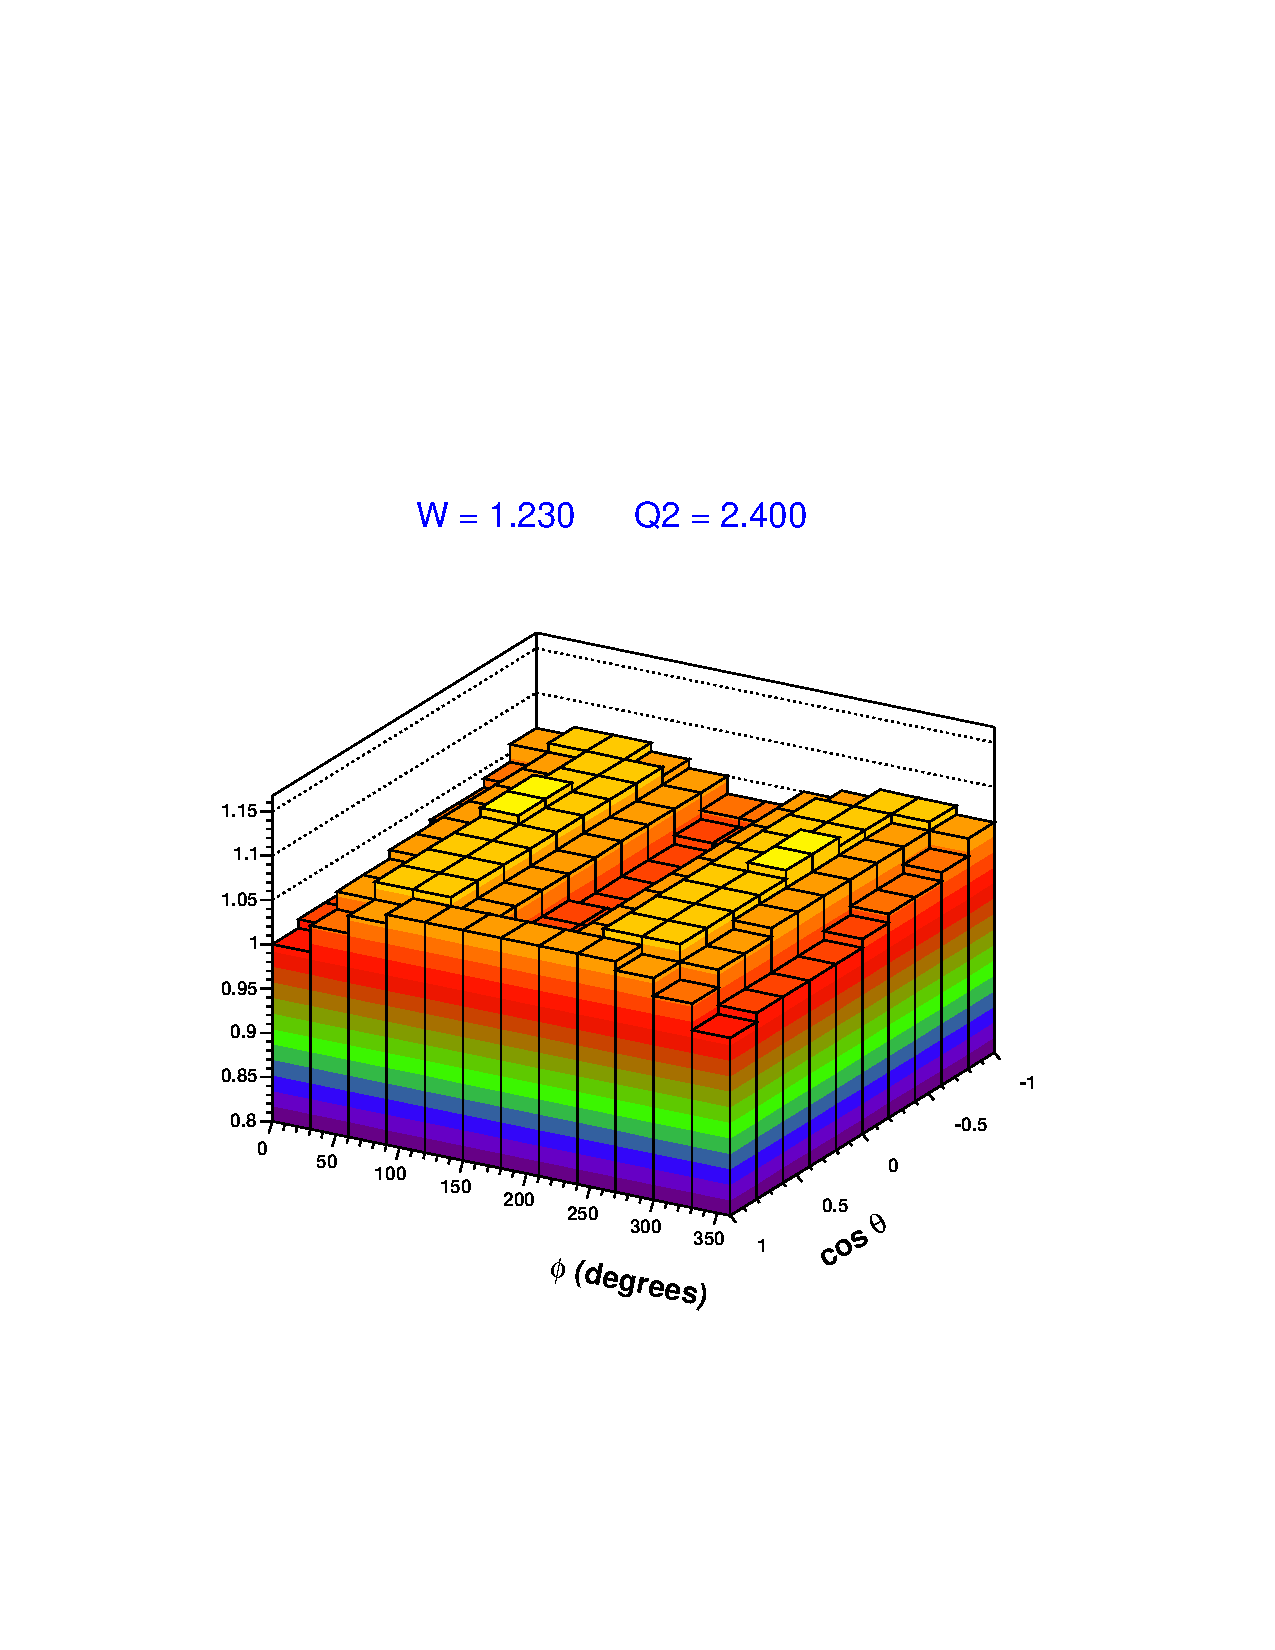
\includegraphics[width = 6.6cm, bb=60 130 520 570]{analysis/img/binave1} \end{minipage}
 \hspace{1cm}
 \begin{minipage}{7cm} 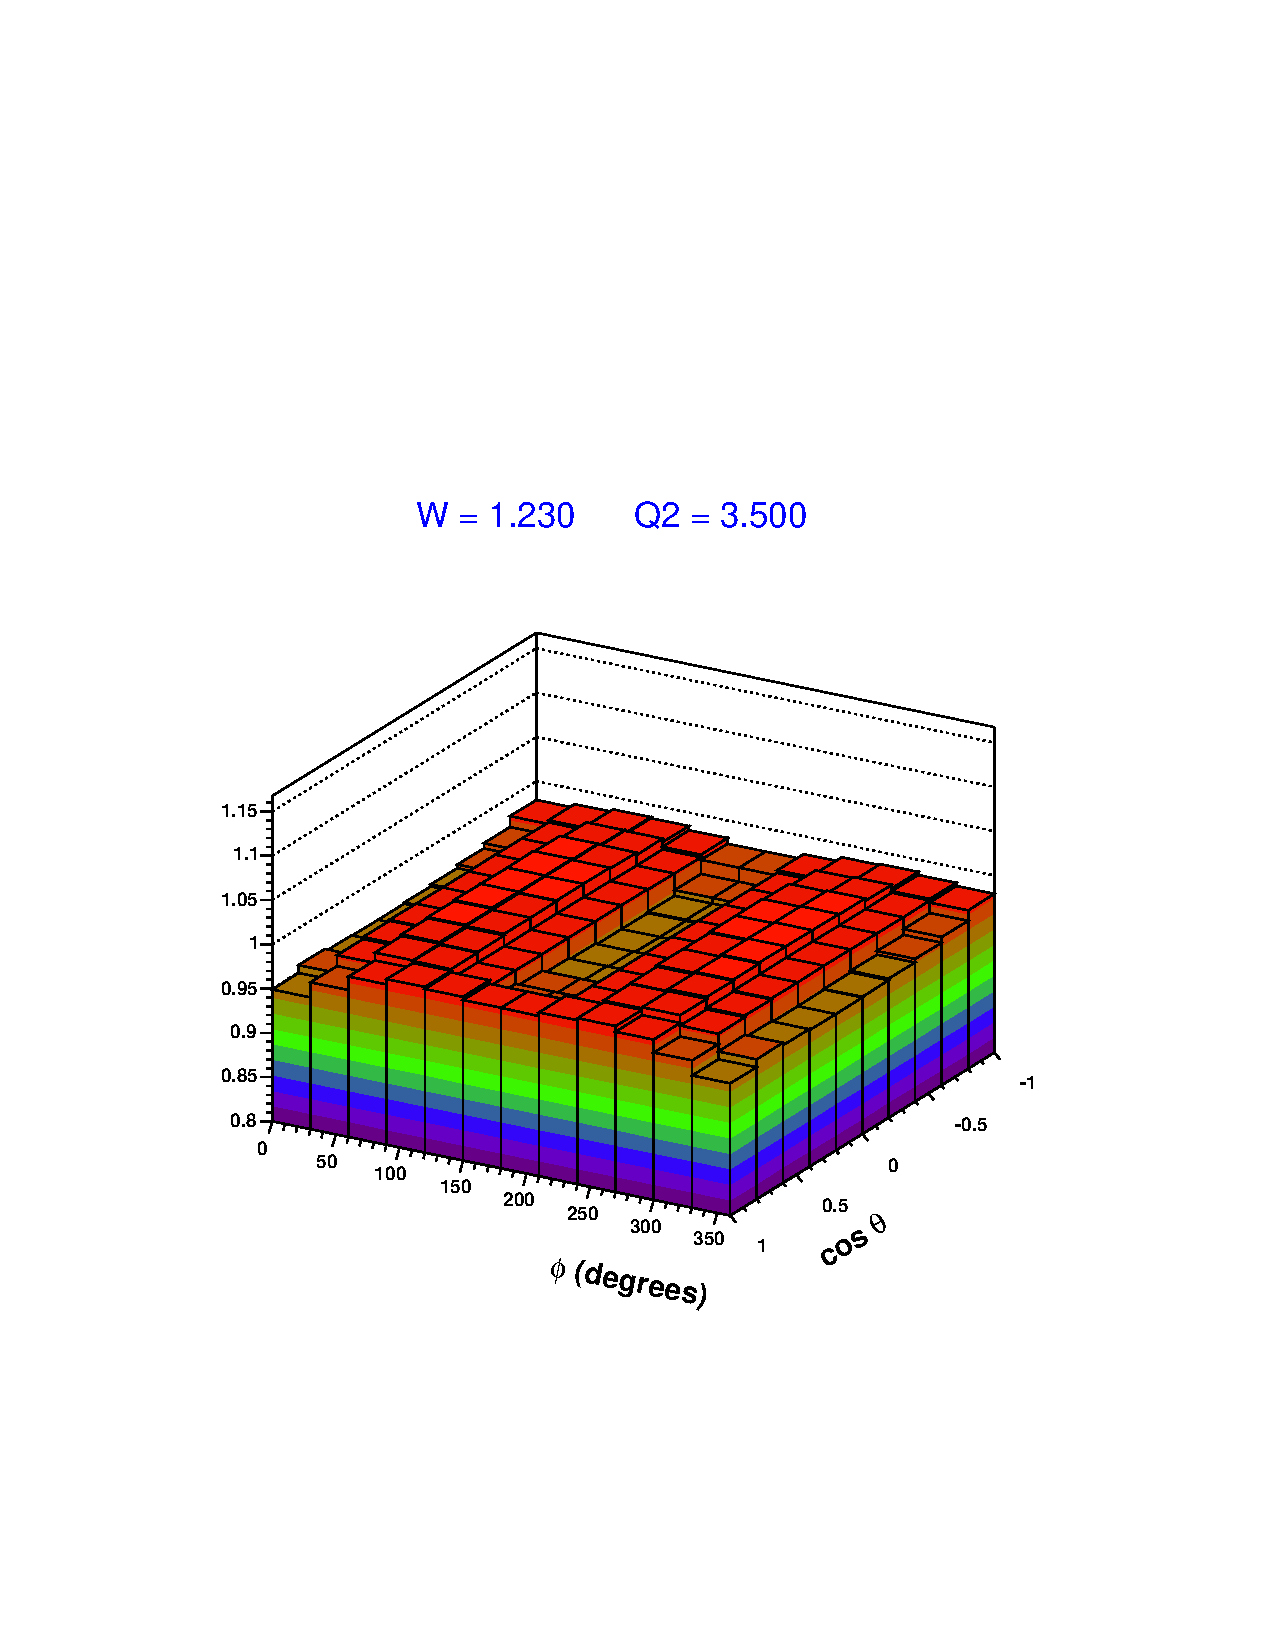
\includegraphics[width = 6.6cm, bb=60 130 520 570]{analysis/img/binave2} \end{minipage}  
 \\
 \vspace{0.1cm}
 \begin{minipage}{7cm} 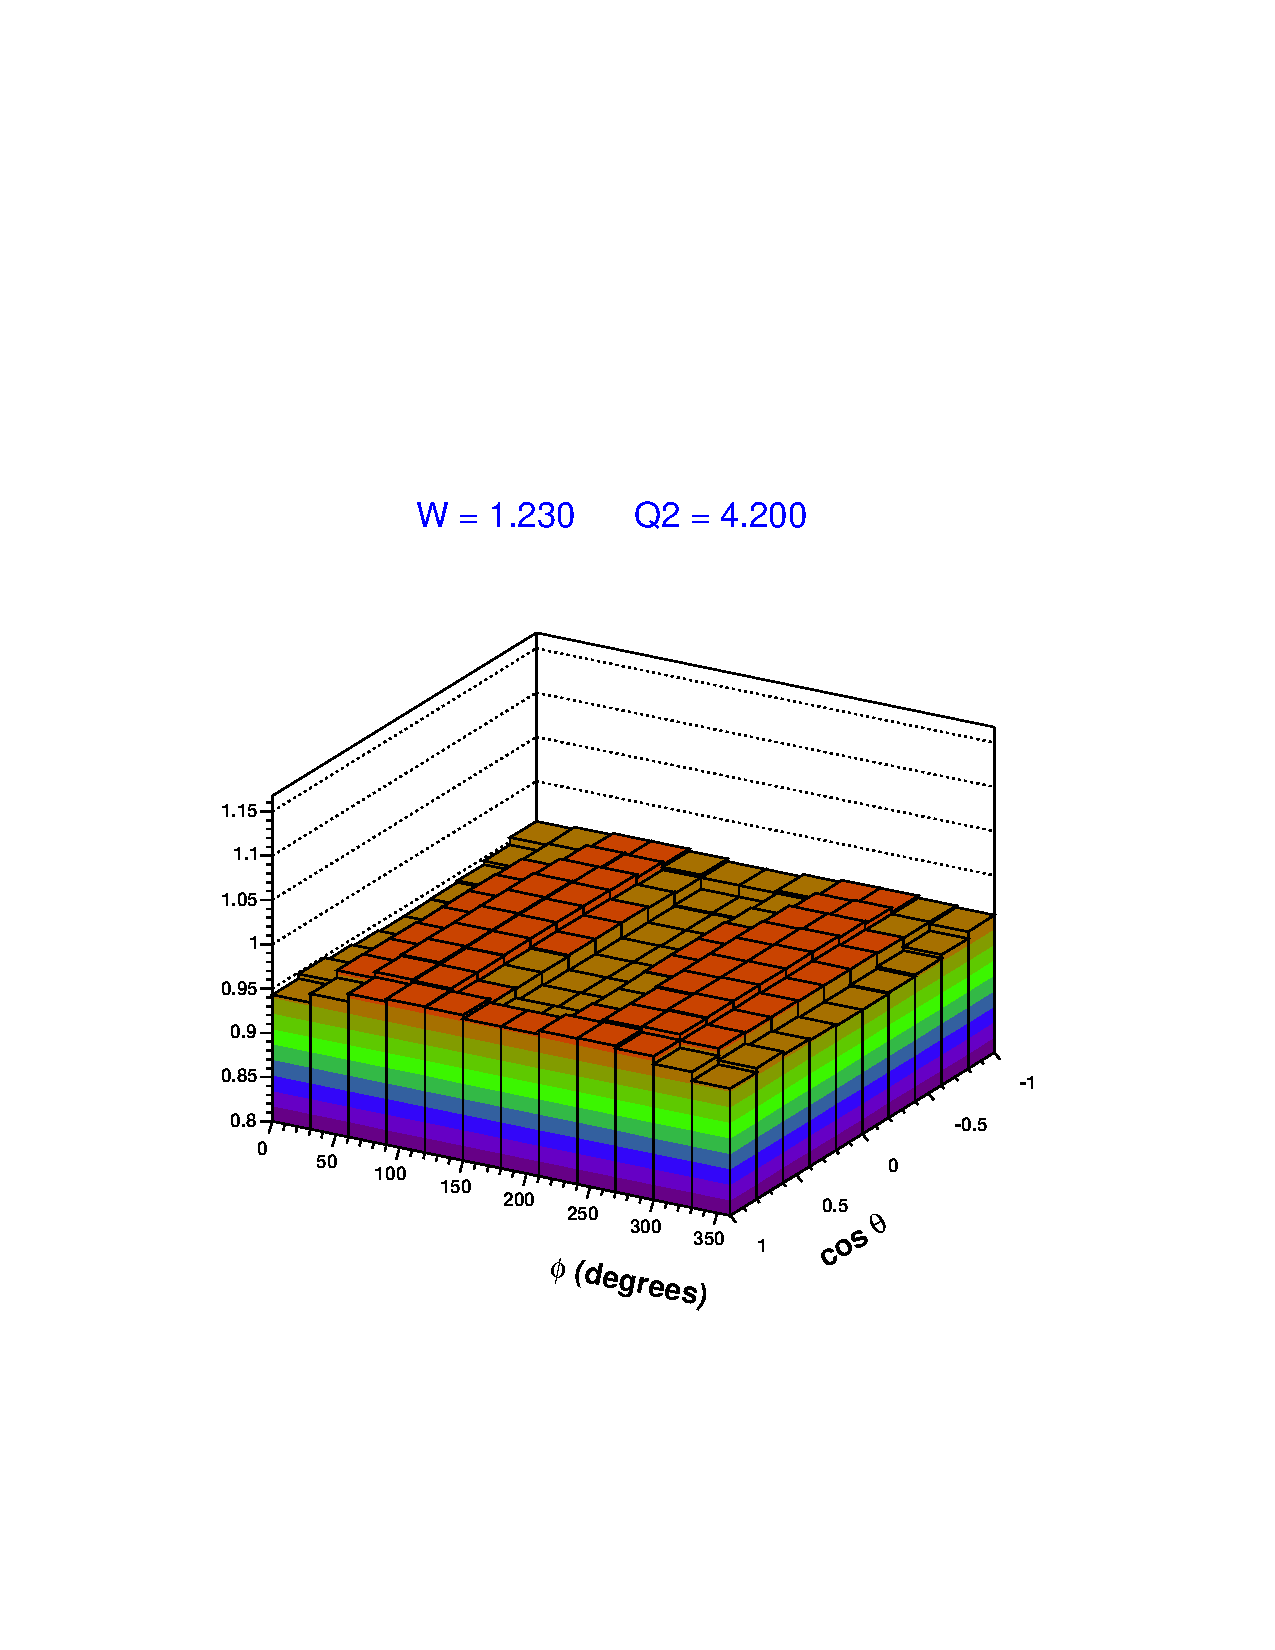
\includegraphics[width = 6.6cm, bb=60 130 520 570]{analysis/img/binave3} \end{minipage}
 \hspace{1cm}
 \begin{minipage}{7cm} 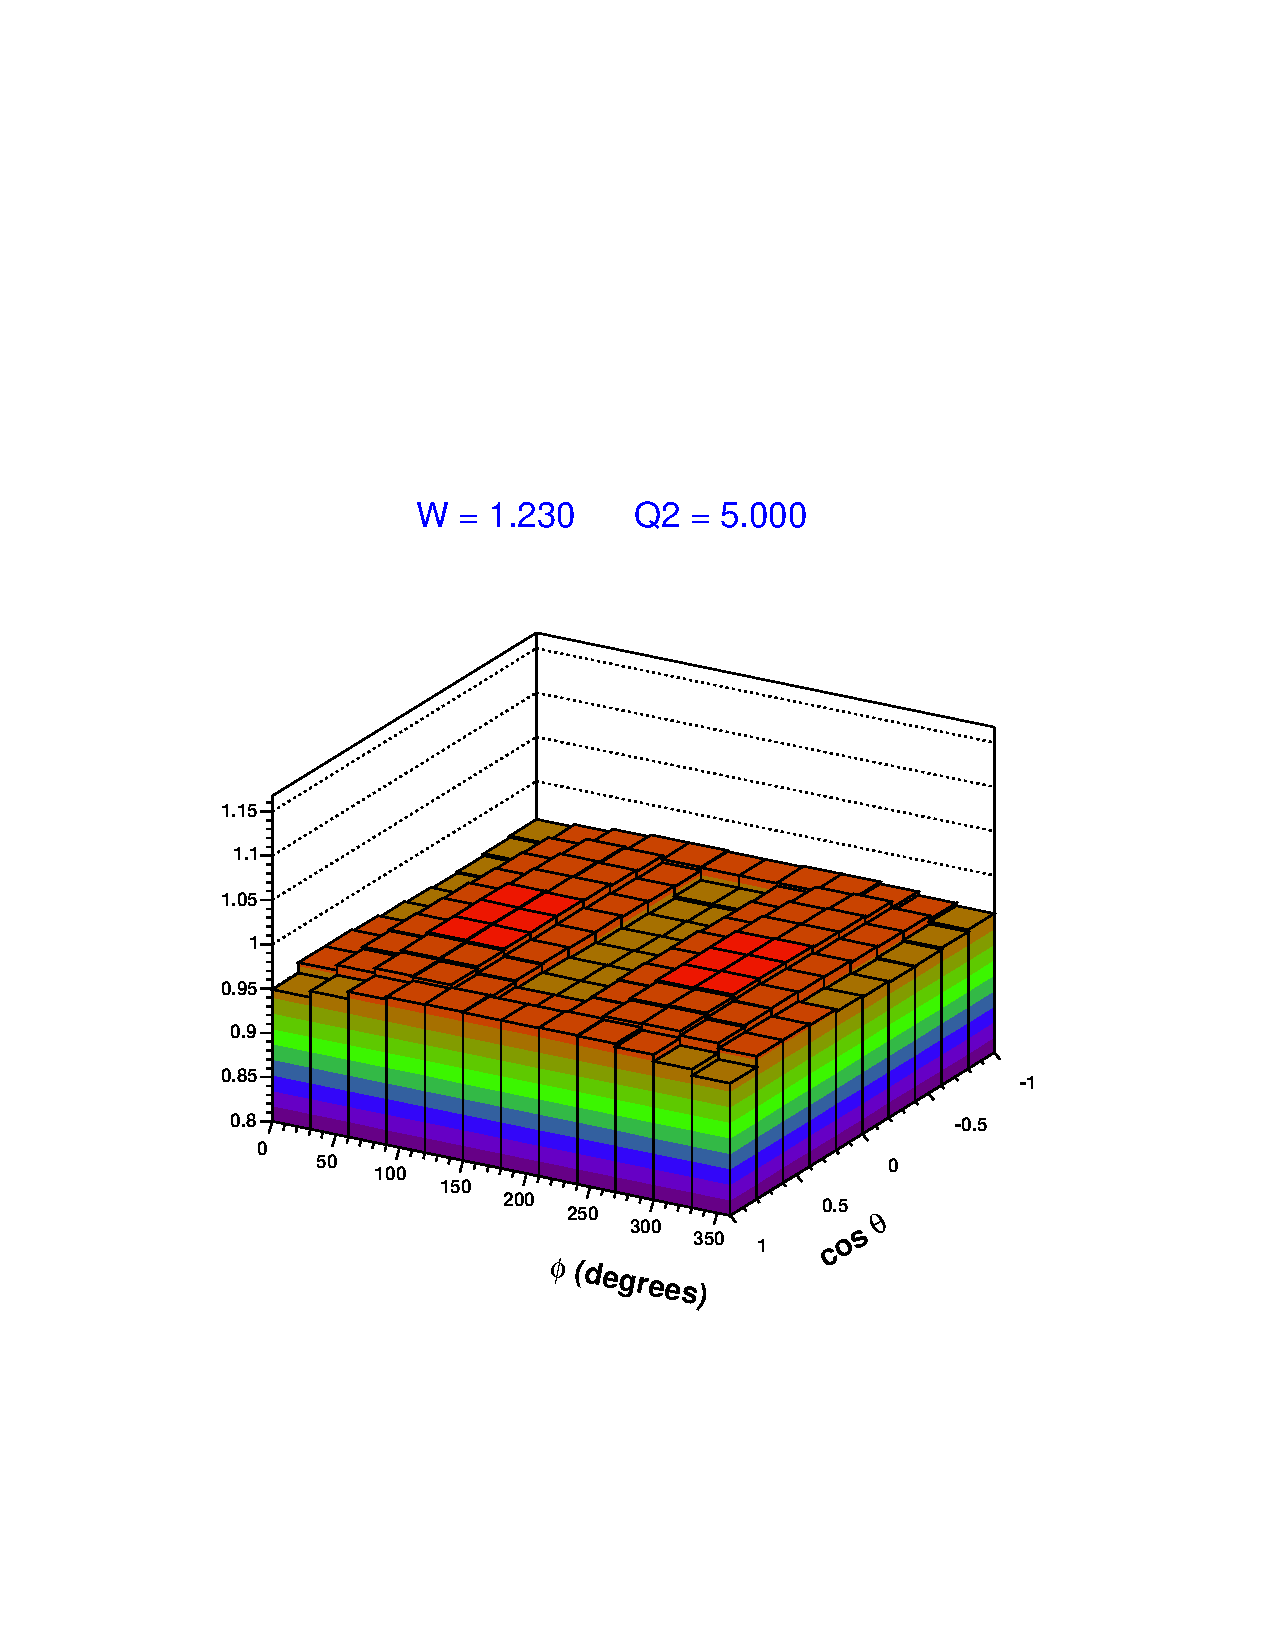
\includegraphics[width = 6.6cm, bb=60 130 520 570]{analysis/img/binave4} \end{minipage}    
  \caption
          { Bin averaging correction.}  
 \label{fig:bin_averaging}
\end{figure}  \\
See    \begin{verbatim} 
http://www.jlab.org/~ungaro/pi0eprod/bin_ave
\end{verbatim}
for the correction in each bin considered as a function of $\phi^*$ or $\cos\theta^*$.










\section{Raw data}
To see the statistic in each bin considered as a function of $\phi^*$ or $\cos\theta^*$
see
See    \begin{verbatim} 
http://www.jlab.org/~ungaro/pi0eprod/raw_plots
\end{verbatim}



\cia\vspace{-2cm}
\section{Radiative correction}
The $\pi^0$ production illustrated in \F{fig:rad} a) is not the only process 
contributing to the electroproduction cross section. A photon or a $e^+e^- $ pair could be produced as well
and the amplitudes of these processes interfere with each other.
The measured $W, Q^2$  changes in case of radiation (for 
example the momentum of a scattered electron that emits a photon differs from the one at the 
leptonic vertex of \F{fig:rad} b) so a {\em radiative correction} is necessary. 


The  following radiative processes are present (in the lowest order of the fine structure constant).
\begin{itemize}
\item
the Bremsstrahlung, \F{fig:rad} b) and c) where a photon is emitted by the incoming or outgoing electron.
\item
the vertex correction, \F{fig:rad} d), where a photon is emitted by the incoming electron and 
absorbed by the outgoing
electron.
\item the vacuum polarization, \F{fig:rad} e), 
where the virtual photon produces temporarily an $e^+e^-$ pair.
\end{itemize}

\begin{figure}[h]
 \begin{center}
  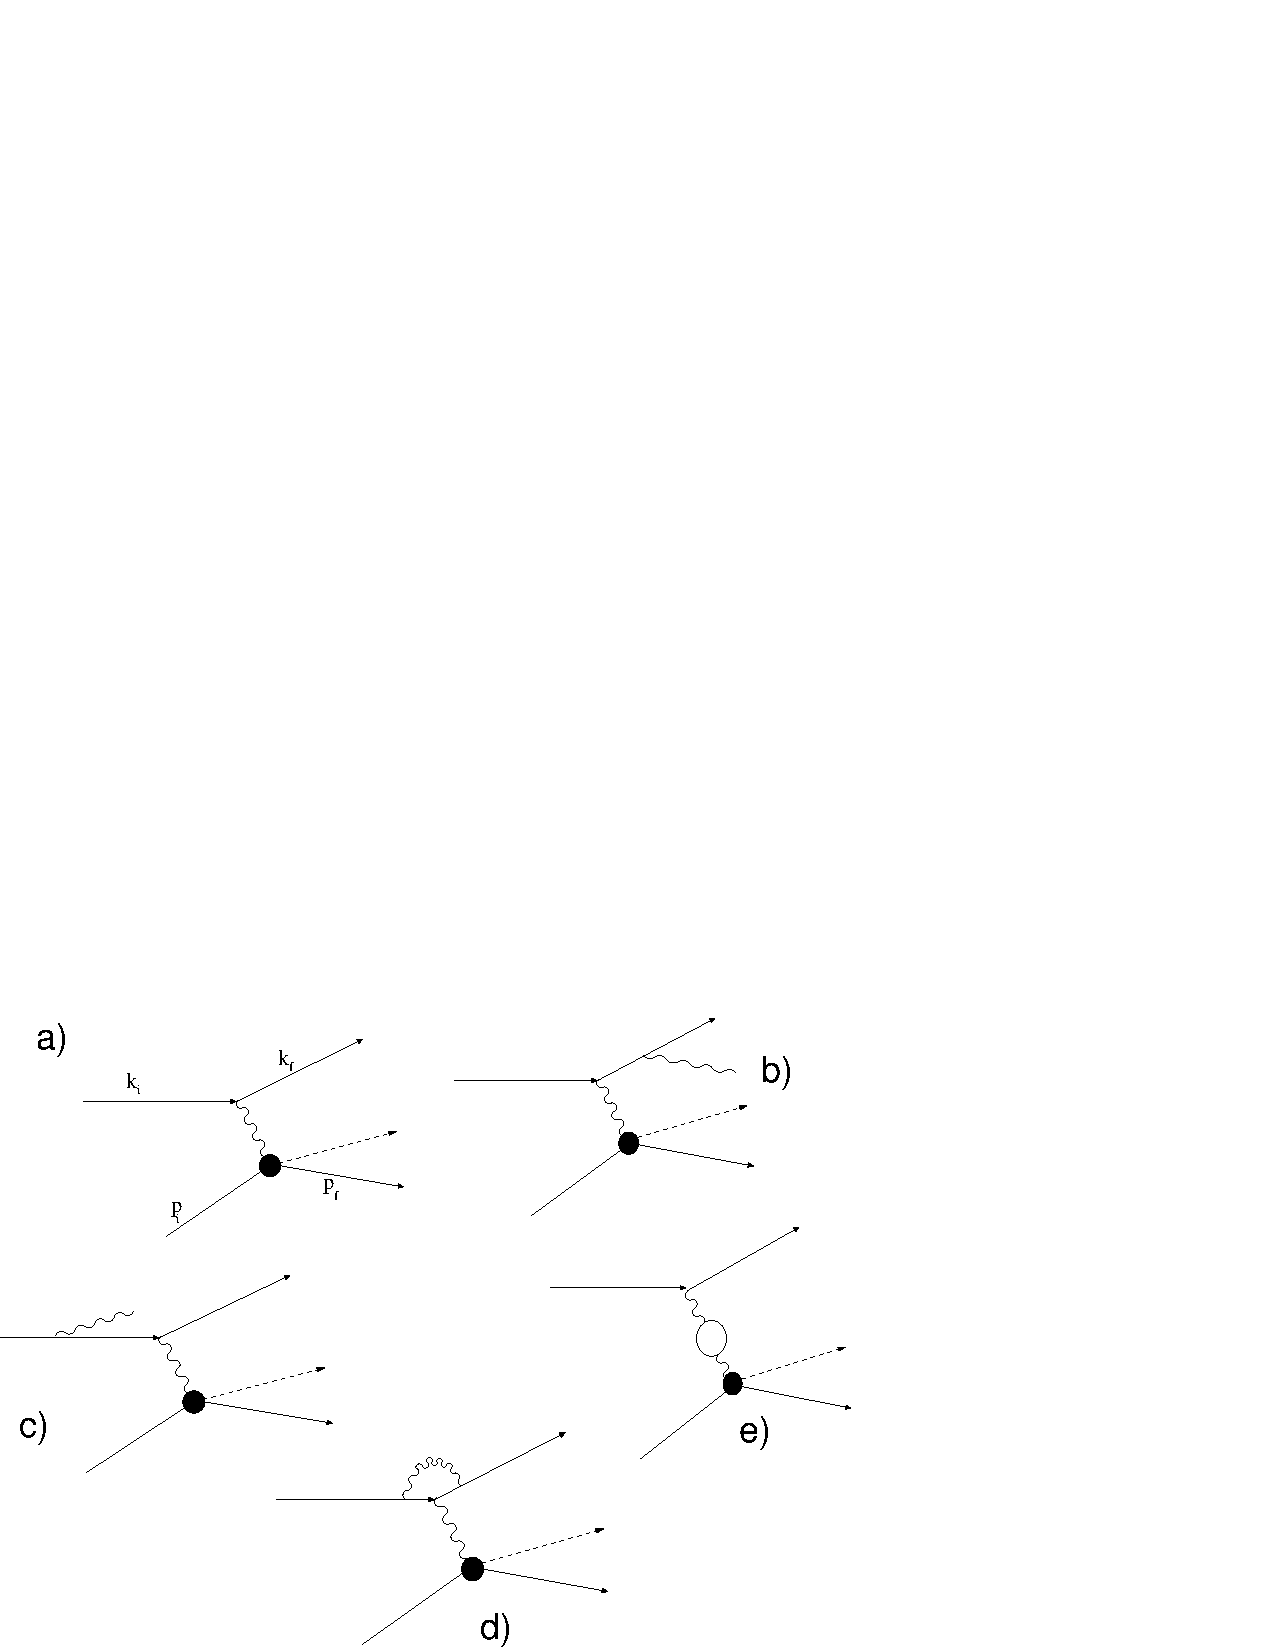
\includegraphics[width=14cm, bb=-60 -40 480 380]{analysis/img/rad}
  \caption[Feynman diagrams for the Born and radiative processes]
          { Feynman diagrams for the Born and radiative processes.
	             a) Born electroproduction, b) and c) Bremsstrahlung d) vertex
		     correction, e) vacuum polarization.}
 \label{fig:rad}
  \end{center} 
\end{figure} 

To account for the radiative processes the approach of reference \cite{bib:radcorr}, which is based on a 
covariant method for infrared cancellation \cite{bib:radinfra}, is used . 
Multiple soft photon radiation is included via exponentiation \cite{bib:shum}, \cite{bib:YFS}.
This method is preferred
over Mo and Tsai the procedure \cite{bib:motsai} because:

\begin{itemize}
\item[1)] It addresses {\it exclusive}
electroproduction rather than inclusive, thus involving all four unpolarized structure functions, as opposed to
the Mo and Tsai formalism which accounts only for two structure functions and inclusive scattering and it is independent of
outgoing hadron angles.
In principle, the general formulas of Mo and Tsai can be adapted to the coincidence framework if the integration
over the photon phase space is done properly. 

\item[2)] The infrared cancellation is independent of the unphysical
parameter $\Delta$ separating the phase space of soft and hard photons 
necessary in the Mo and Tsai procedure and leading to uncertainties.

\item[3)] The approach of ref. \cite{bib:radcorr} does not rely on the peaking approximation, avoiding
uncertainties at a few percent level associated with it.

\end{itemize}

The matrix element of the unradiated process \F{fig:rad} a) can be written as
\begin{equation}
 M^2 = \Dfrac{e^4}{Q^4}L_{\mu\nu}W^{\mu\nu}
 \label{eqno:mzero}
\end{equation}
where $L_{\mu\nu}$ and $W^{\mu\nu}$ are the leptonic and hadronic tensors:
\begin{equation}
L_{\mu\nu} = \Dfrac{1}{2}\,Tr\,(\slashed{k}_f+m)\gamma_\mu(\slashed{k}_i+m)(1+{\it i}\gamma_5\xi)\gamma_\nu 
\label{eqno:lepttens}
\end{equation}

The leptonic tensor for the radiative processes illustrated in \F{fig:rad} b), c), d) and e) changes into
\begin{equation}
L_{\mu\nu}^R = \Dfrac{1}{2}\,Tr\,(k_f+m)\Gamma_{\mu\alpha}(k_i+m)(1+{\it i}\gamma_5\xi)\hat{\Gamma}_{\alpha\nu}
\end{equation}
where the tensor $\Gamma_{\mu\alpha}$ contains the photon information $k^\mu_\gamma$.

The contraction of $L_{\mu\nu}^R$ with  $W^{\mu\nu}$ gives the matrix element $ M^2_R $ for the radiative processes:

\begin{equation}
 M^2_R = -\Dfrac{2e^6}{\tilde{Q}^4}L_{\mu\nu}^RW^{\mu\nu} =  -\Dfrac{2e^6}{\tilde{Q}^4R_w} \sum_{i=1}^{5}\theta_i H_i
 \label{eqno:radcorr}
\end{equation}
where $\tilde{Q^2} = -(q-k_\gamma)^2$ and $R_w = W^2 - (p+q-k_\gamma)^2$. One can see the involvement of all 
the structure functions $H_i$ and the intuitive modification to the normal definitions of $\tilde{Q^2}$ and $R_w$
with the presence of a radiated photon.

\begin{figure}[h]
 \begin{center}
  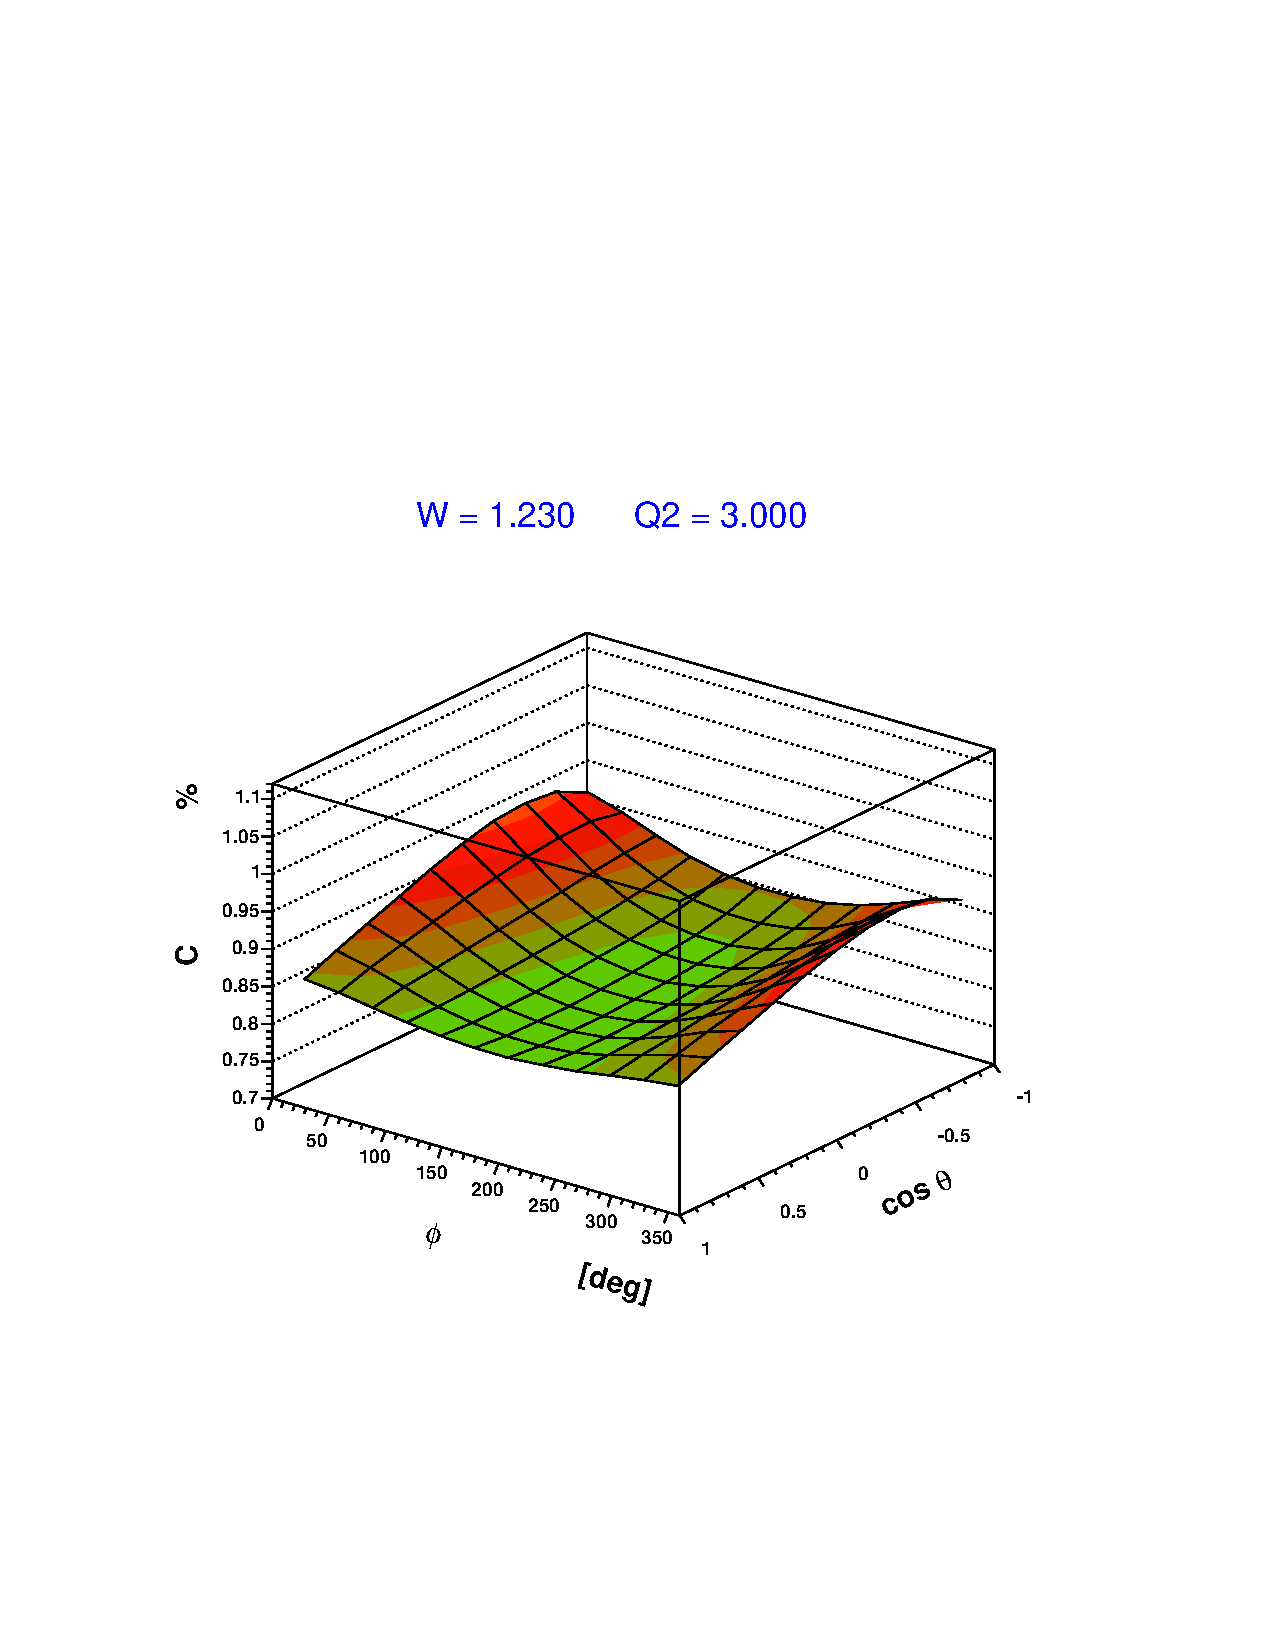
\includegraphics[width=15cm, bb=0 130 540 600]{analysis/img/costheta_phi_radcor_w1.23_q3.00}
  \caption[Radiative correction as a function of $\cos\theta^*$ and $\phi^*$ for $W=1.23$ GeV and $Q^2=3$ GeV$^2$]
          { Radiative correction as a function of $\cos\theta^*$ and $\phi^*$ for $W=1.23$ GeV and $Q^2=3$ GeV$^2$.}
 \label{fig:costheta_phi_radcor_w1.23_q3.00}
  \end{center} 
\end{figure} 

A program named {\it EXCLURAD} which is described in \cite{bib:radcorr} has been developed to calculate the matrix element (\ref{eqno:radcorr}) using
existing models (like MAID or DMT) for the structure functions. This program gives the radiative correction C as the ratio of the radiative
and unradiative four fold cross section:
$$
C(W, Q^2, \cos\theta^*, \phi^*) =\Dfrac{\sigma_{RAD}}{\sigma_{UNRAD}}
$$
which has been used as the radiative correction in this analysis.
Dependance on the missing mass cutoff parameter is tacit.
\F{fig:costheta_phi_radcor_w1.23_q3.00} shows the correction as a function 
of $\cos\theta^*$ and $\phi^*$ for $W=1.23$ GeV and $Q^2=3$ GeV$^2$.
Note that this procedure is different from that one followed for our published lower $Q^2$ data.
See    \begin{verbatim} 
http://www.jlab.org/~ungaro/pi0eprod/rad_plots/
\end{verbatim}
for the correction in each bin considered as a function of $\phi^*$ or $\cos\theta^*$.


































%\cia\vspace{-2cm}
\section{Absolute normalization of the cross section}
\subsection{Accumulated Faraday Cup}
During the data acquisition the beam charge impinging on the target was saved in the data 
stream as accumulated charge, corrected for live-time by a Faraday cup reading located in the beam dump.
This is a particular event in the data stream called {\it scaler} event.
It consist of a counter whose output $F_{CUP}$ is proportional to the accumulated charge by the relation:
$$
Q^i (Coulombs) = \Dfrac{F^i_{CUP}}{9264.0 \cdot 10^9}
$$
The $F_{CUP}$ reading is performed approximately every 10 second, and it is labelled with an event number
$i$.

Since one run was typically divided into several files, it is possible that the last
Faraday cup reading does not correspond to the accumulated charge for the run because
of corrupted i/o (for example one file can be lost). This is a rare occurence
but must be taken into account. 

To calculate the Faraday cup for a run the difference between
one scaler reading and the next is calculated and saved
$$
\Delta F_{CUP} = F_{CUP}^{i'} - F_{CUP}^i
$$ 
only when $i' = i+1$ (otherwise $\Delta F_{CUP}=0$ ). The $\Delta F_{CUP}$ obtained is then summed 
over all scaler events. \\

For the e1-6 running period the total Faraday cup reading was $F_{CUP} = 2.06816e+11$ for a total charge
$$
Q = 0.022325\;\;{\rm Coulomb}
$$
Assuming a constant current $I=7\,nA$ this gives a running time $t=Q/c\sim 3.2 M {\rm sec} \sim 37$ days.
The number of accelerated electrons was
$$
n_e = Q/e = 1.3934 \cdot 10^{17}
$$
where $e$ is the electron charge.
The number of target nuclei per $cm^2$ can be calculated with the formula:
$$
n_P = \Dfrac{L\,\rho\,N_A}{a.m.u.}
$$
where $L=5$ cm is the length of the target, $\rho=0.0708$ g/cm$^3$ is the density of $H_2$ at $20$K,
$A= 6.022\cdot10^{23}$ mol$^{-1}$ is the Avogadro number and $a.m.u. = 1.00794$ g/mol is the atomic mass unit 
of the hydrogen.
This gives
$$
n_P = 2.115\cdot 10^{23} {\rm cm^{-2}}
$$
So the integrated luminosity for the e1-6 period was
$$
L_{int} = 2.95\cdot 10^{40} {\rm cm^{-2}}
$$

\subsection{Check of normalization}
To estimate the quality of the normalization a comparison of the data with
previous measured and theoretical total c.m. cross sections at lower $Q^2$ is performed.
Equation (\ref{eqno:diffcross}) can be  integrated
over d$\Omega ^*$ to find out that the total cross section is proportional to
$|M_{1+}|^2$:

\begin{equation}
\sigma_{TOT}^{\pi^0} = 8\pi\, \, \Dfrac{2W}{W^2-m_P^2} \,\, |M_{1+}|^2
\end{equation}
so that $|M_{1+}|^2$ can be used as normalization check.

\F{fig:MM} shows the $|M_{1+}|^2$ at the peak of the $\Delta$ as a function of $Q^2$.
The data from \cite{bib:frolov} and the MAID and DMT predictions are also shown.
Good agreement is found with previous results and the two models.

\begin{figure}[h]
 \begin{center}
  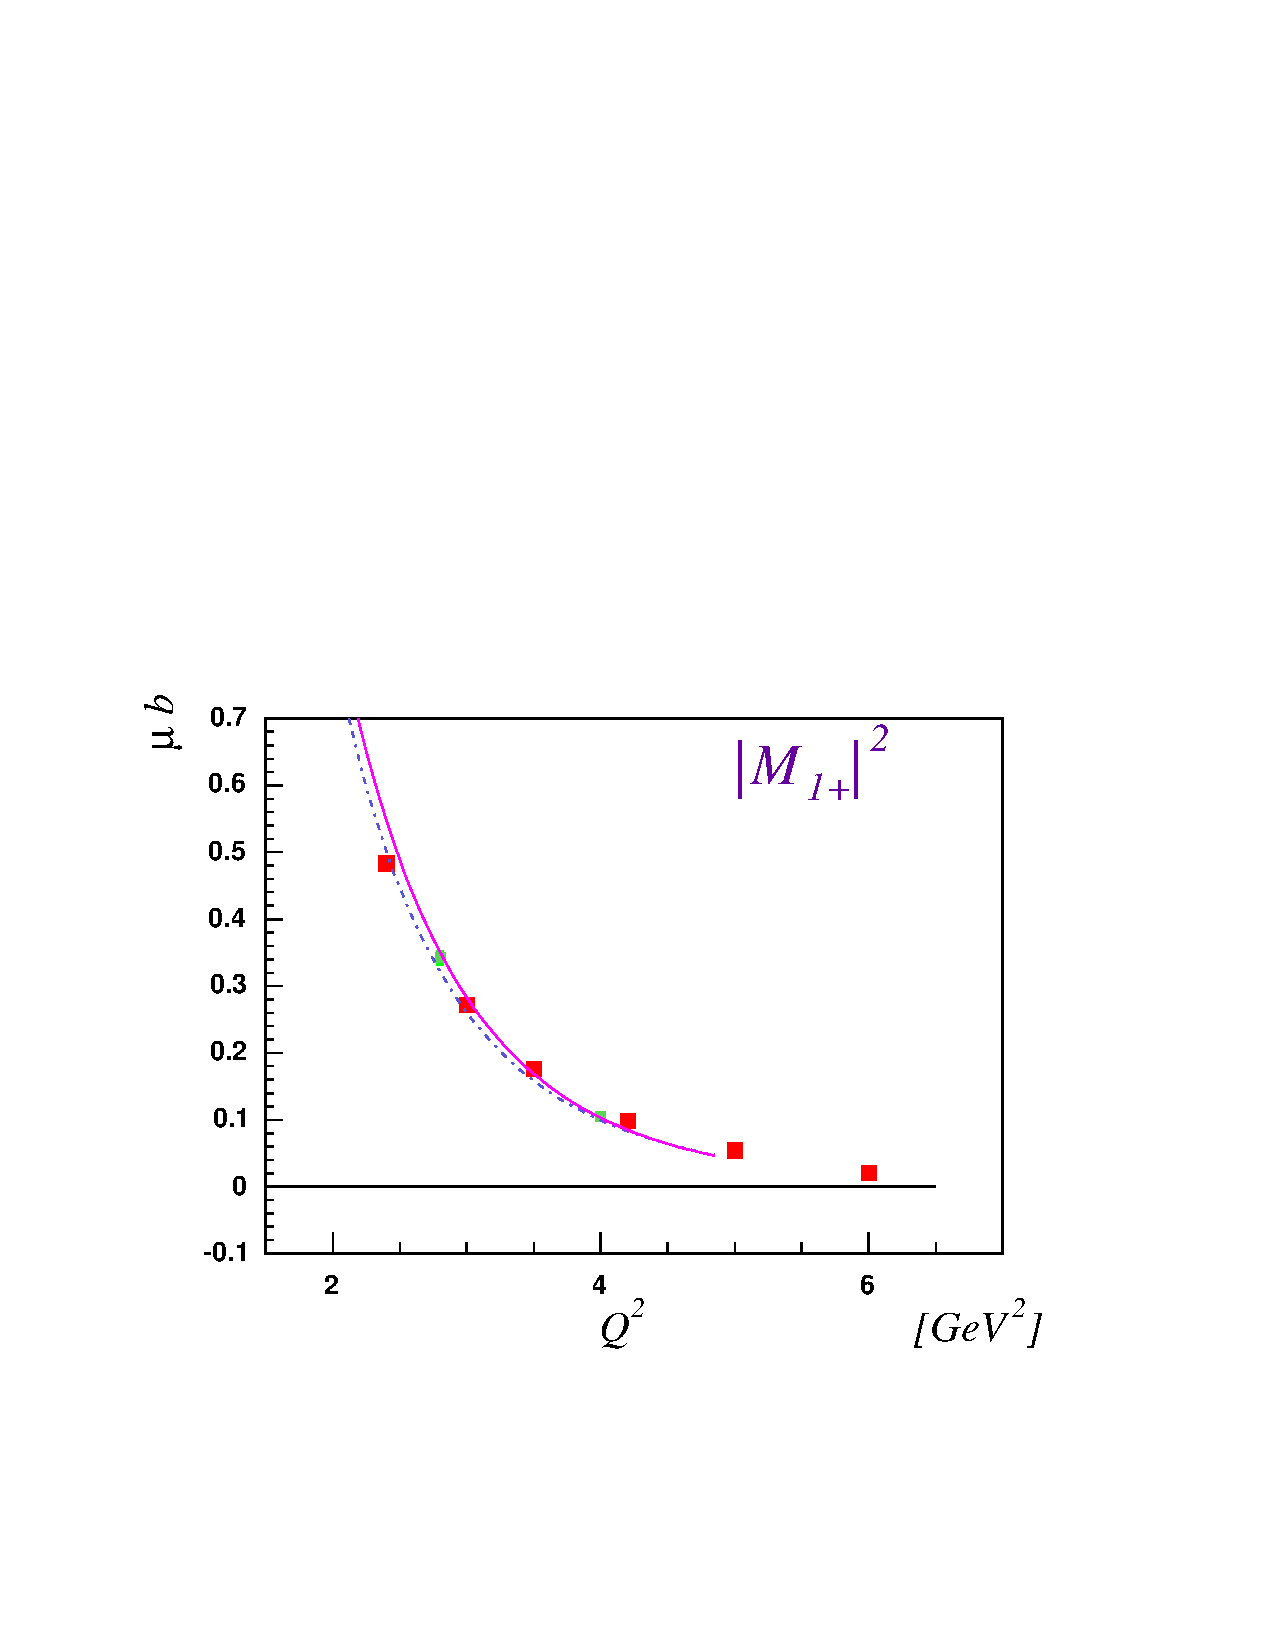
\includegraphics[width=14cm, bb=40 100 520 460]{analysis/img/MM}
  \caption[$|M_{1+}|^2$ at the peak of the $\Delta$ as a function of $Q^2$]
          { $|M_{1+}|^2$ at the peak of the $\Delta$ as a function of $Q^2$.
	             The green points come from \cite{bib:frolov}. The solid line is due to MAID, 
		     the dashed line is due to DMT.}
 \label{fig:MM}
  \end{center} 
\end{figure} 






















\section{Extraction of the structure functions}
\label{sec:structure}
The $\pi^0$ differential cross section in the 
resonance center of mass assumes the form

\begin{equation}
\Dfrac{d\sigma}{d\Omega^*_{\pi^0}} = \Dfrac{2W p^*_{\pi^0}}{W^2-m_P^2}\left( \sigma_T + \epsilon\sigma_L
+\epsilon\sigma_{TT}sin^2\theta cos2\phi +
\sigma_{LT}\sqrt{2\epsilon_L(\epsilon+1)}sin\theta cos\phi \right)
\end{equation}

where  $\phi$ and $\theta$ are the azimuthal and polar angle of the $\pi^0$ in the c.m. frame
and  $\sigma_T$, $\sigma_L$, $\sigma_{LT}$, $\sigma_{TT}$   are the structure functions.
The $\phi$ distributions are modulated only by the terms $\cos\phi$ and $\cos 2\phi$ while all the other
terms vary with $W$, $Q^2$ and $\cos\theta$ (but not with $\phi$).
Therefore the structure functions can be extracted with a $\phi$ fit.

For each $W$, $Q^2$ and $\cos\theta$ bin the 
quantity in parenthesis is fitted with the functional form
\begin{equation}
 y = a + b\cos\phi + c\cos 2\phi
\end{equation}
The structure functions are then calculated with the formulas:
\begin{equation}
\begin{array}{l l l}
\sigma_T + \epsilon\sigma_L & = & a \\
& & \\
\sigma_{LT}                 & = & \Dfrac{b}{\sin\theta\sqrt{2\epsilon_L(\epsilon + 1)}} \\
& & \\
\sigma_{TT}                 & = & \Dfrac{c}{\sin^2\theta \epsilon_T}
\end{array}
\end{equation}
See    \begin{verbatim} 
http://www.jlab.org/~ungaro/pi0eprod/cro_plots
\end{verbatim}
for the cross section plots in each bin considered and for different cuts applied
during this analysis.




\F{fig:bac_phi_W1.23_Q22.40} shows the $\phi$ fits of the cross section for $W=1.1\,\pm\,0.01$ GeV and $Q^2 = 2.4$ GeV$^2$.

\F{fig:chi2_ctr} shows the  $\chi^2/\nu$ distribution for all the fits at different $Q^2$ 
values (black points) along with the expected $\chi^2/\nu$ distribution (red line)
\begin{equation}
\chi^2/\nu(x) = \Dfrac{2}{2^{\nu /2} \Gamma(\nu /2)} \, x^{\nu-1}\, e^{-x^2/2}
\end{equation}



There are 12 bins in $\phi$ and there  are 3 fit paramters therefore
$$
 \nu = {N-{\rm constraints}} = 9.
$$
\F{fig:Sigma_lpt_Q2_2.40} shows $\sigma_L + \epsilon\sigma_T$ resulting from the fit at $Q^2 = 2.4$ GeV$^2$.

\begin{figure}[h]
 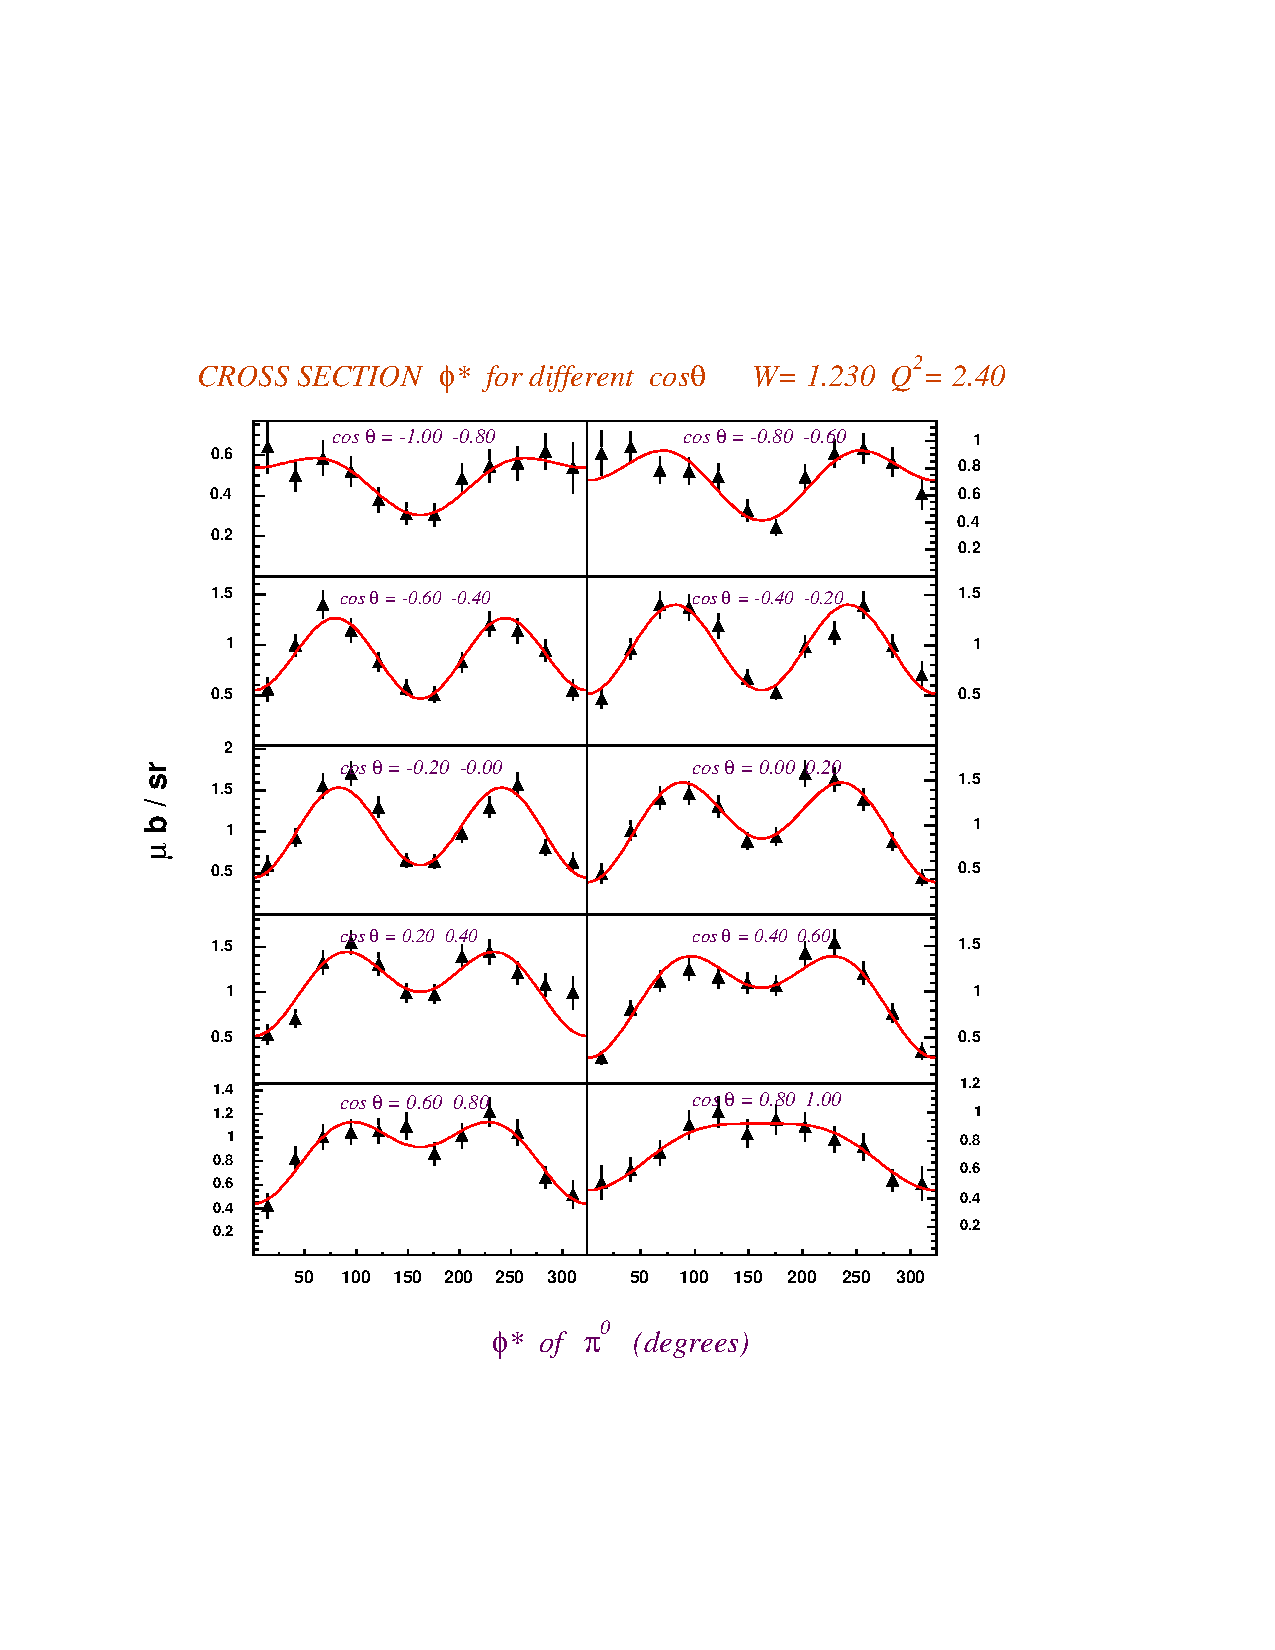
\includegraphics[width = 11cm, bb=60 120 420 640]{analysis/img/bac_phi_W1.23_Q22.40}
  \caption[$\phi$ fits of the cross section for different $\cos\theta$ values]
          { $\phi$ fits of the cross section for different $\cos\theta$ values.
	             The function used for the fit is $ y = a + b\cos\phi + c\cos 2\phi$
		     and the structure functions follow from the parameters $a,b,c$.}
 \label{fig:bac_phi_W1.23_Q22.40}

\end{figure}
\cia

\begin{figure}[h]
 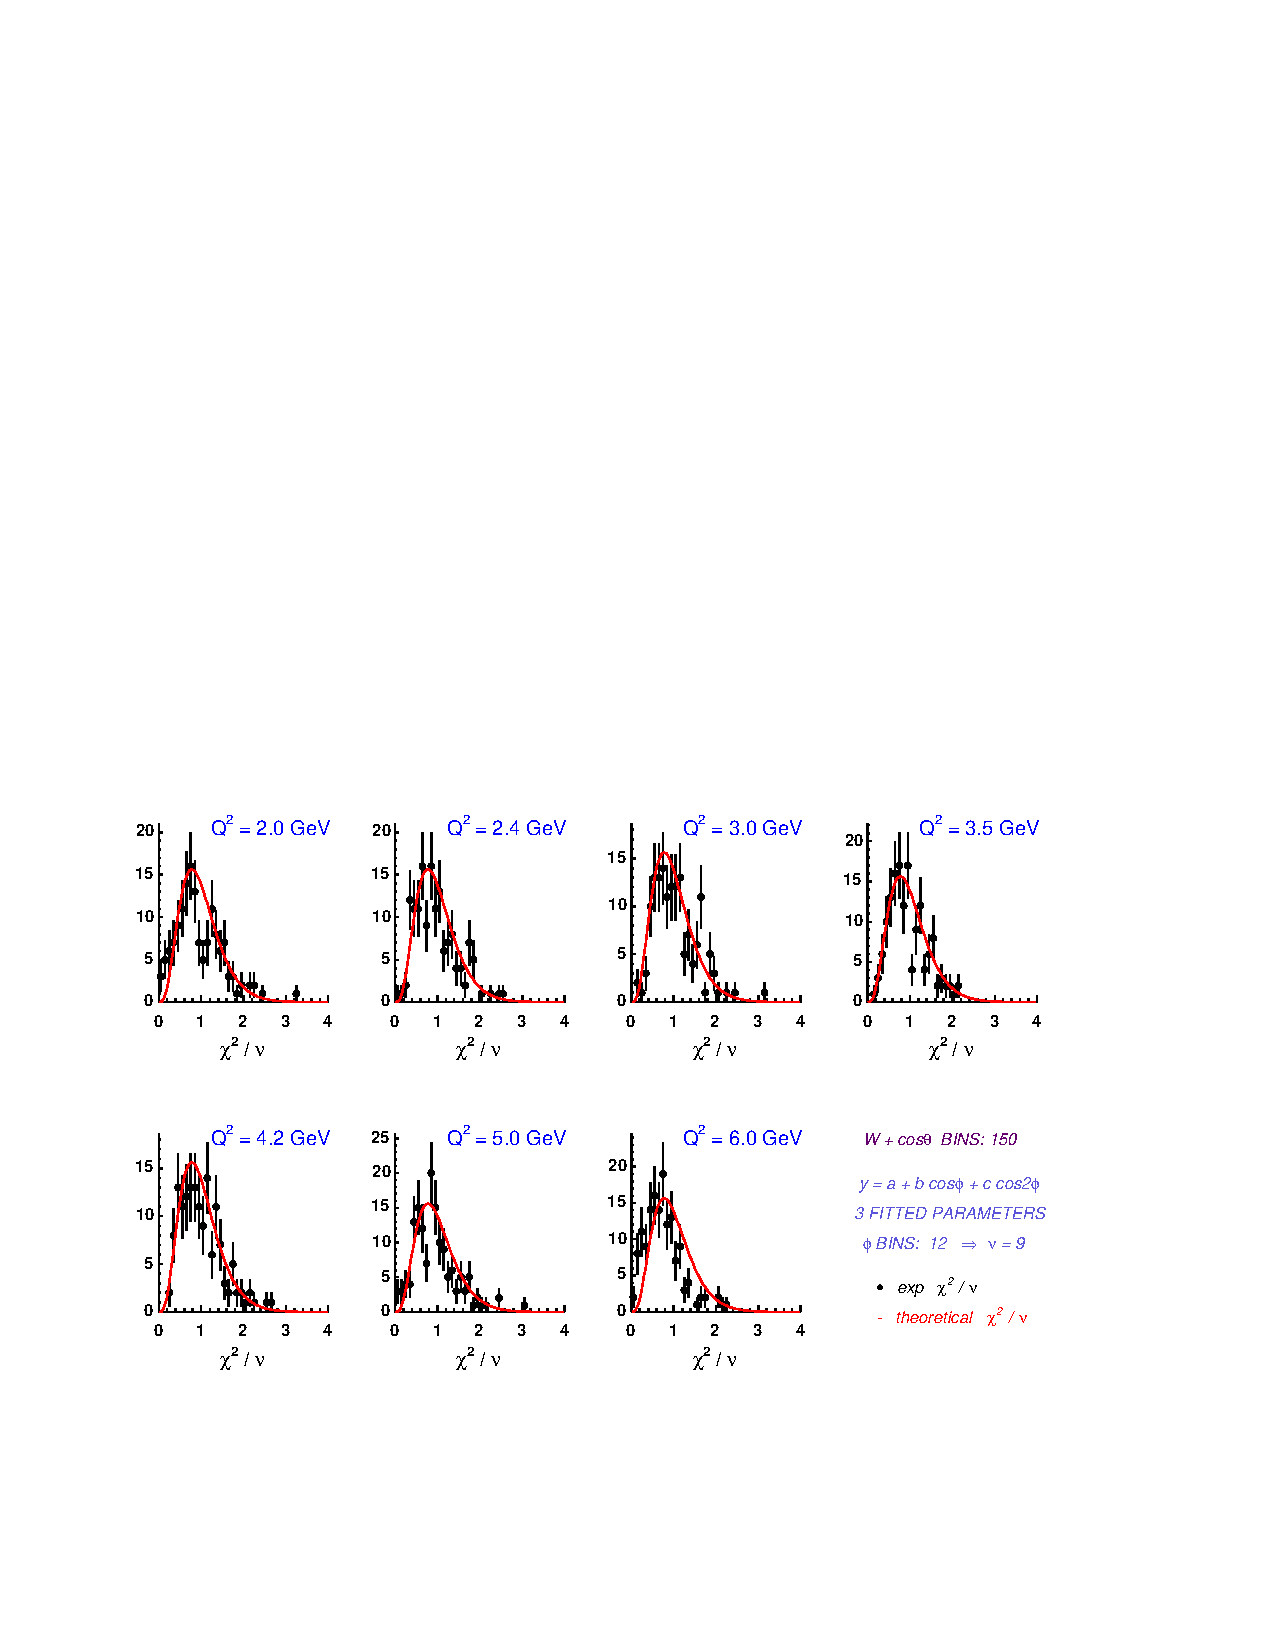
\includegraphics[width = 11cm, bb=50 110 380 400]{analysis/img/chi2_ctr} 
  \caption[Reduced $\chi^2$ distribution of the $\phi$ fits]
          { Reduced $\chi^2$ distribution of the $\phi$ fits. The distributions
	             show consistency with the expected  $\chi^2$ distribution for 150 fits
		     (15 W bins and 10 $\cos\theta$ bins) and 9 degrees of freedom.}
 \label{fig:chi2_ctr}
\end{figure}





\section{Multipole Truncation Analysis}
While the extraction of the structure functions is model independent, 
assumptions on the partial waves of the background and other resonances have to be made
in order to extract quantities such as the coefficients of the legendre expansion of the 
structure functions or the electromagnetic multipoles.
 

\subsection{Legendre expansion}
\label{sec:legendre}
In order to extract the multipoles, the structure functions were fitted
with orthogonal Legendre polynomials with $\ell$ up to d-waves (both the cases
$\ell\le 1$ and $\ell \le 2$ have been considered).
In the case of $\ell \le 1$ the expansion is:
$$
\begin{array}{l c l}
\sigma_T + \epsilon\sigma_L & = & A_0 + A_1P_1(cos\theta) + A_2P_2(cos\theta) \\
\sigma_{TT}                 & = & C_0 \\
\sigma_{LT}                 & = & D_0 + D_1P_1(cos\theta)  \\
\end{array}
$$

In the case of $\ell \le 2$ the expansion is:
$$
\begin{array}{l c l}
\sigma_T + \epsilon\sigma_L & = & A_0 + A_1P_1(cos\theta) + A_2P_2(cos\theta) + A_2P_3(cos\theta) + A_3P_4(cos\theta)\\
\sigma_{TT}                 & = & C_0 + C_1P_1(cos\theta) \\
\sigma_{LT}                 & = & D_0 + D_1P_1(cos\theta) + D_2P_2(cos\theta) \\
\end{array}
$$


Figures \ref{fig:Sigma_lpt_Q2_2.40},  \ref{fig:Sigma_tt_Q2_2.40} and \ref{fig:Sigma_lt_Q2_2.40} show 
the fits for $\sigma_L + \epsilon\sigma_T$, $\sigma_{TT}$ and $\sigma_{LT}$ for different 
$W$ at $Q^2 = 2.4$ GeV$^2$. 
\F{fig:chi2_rtm} shows the obtained and the expected $\chi^2/\nu$ distributions for the various response functions.

To see the fits for $\sigma_L + \epsilon\sigma_T$, $\sigma_{TT}$ and $\sigma_{LT}$ for all the 
$Q^2$ bins and $\ell\le 1$ and $\ell \le 2$ cases, see
\begin{verbatim} 
http://www.jlab.org/~ungaro/pi0eprod/responses
\end{verbatim}

\begin{figure}[h]
 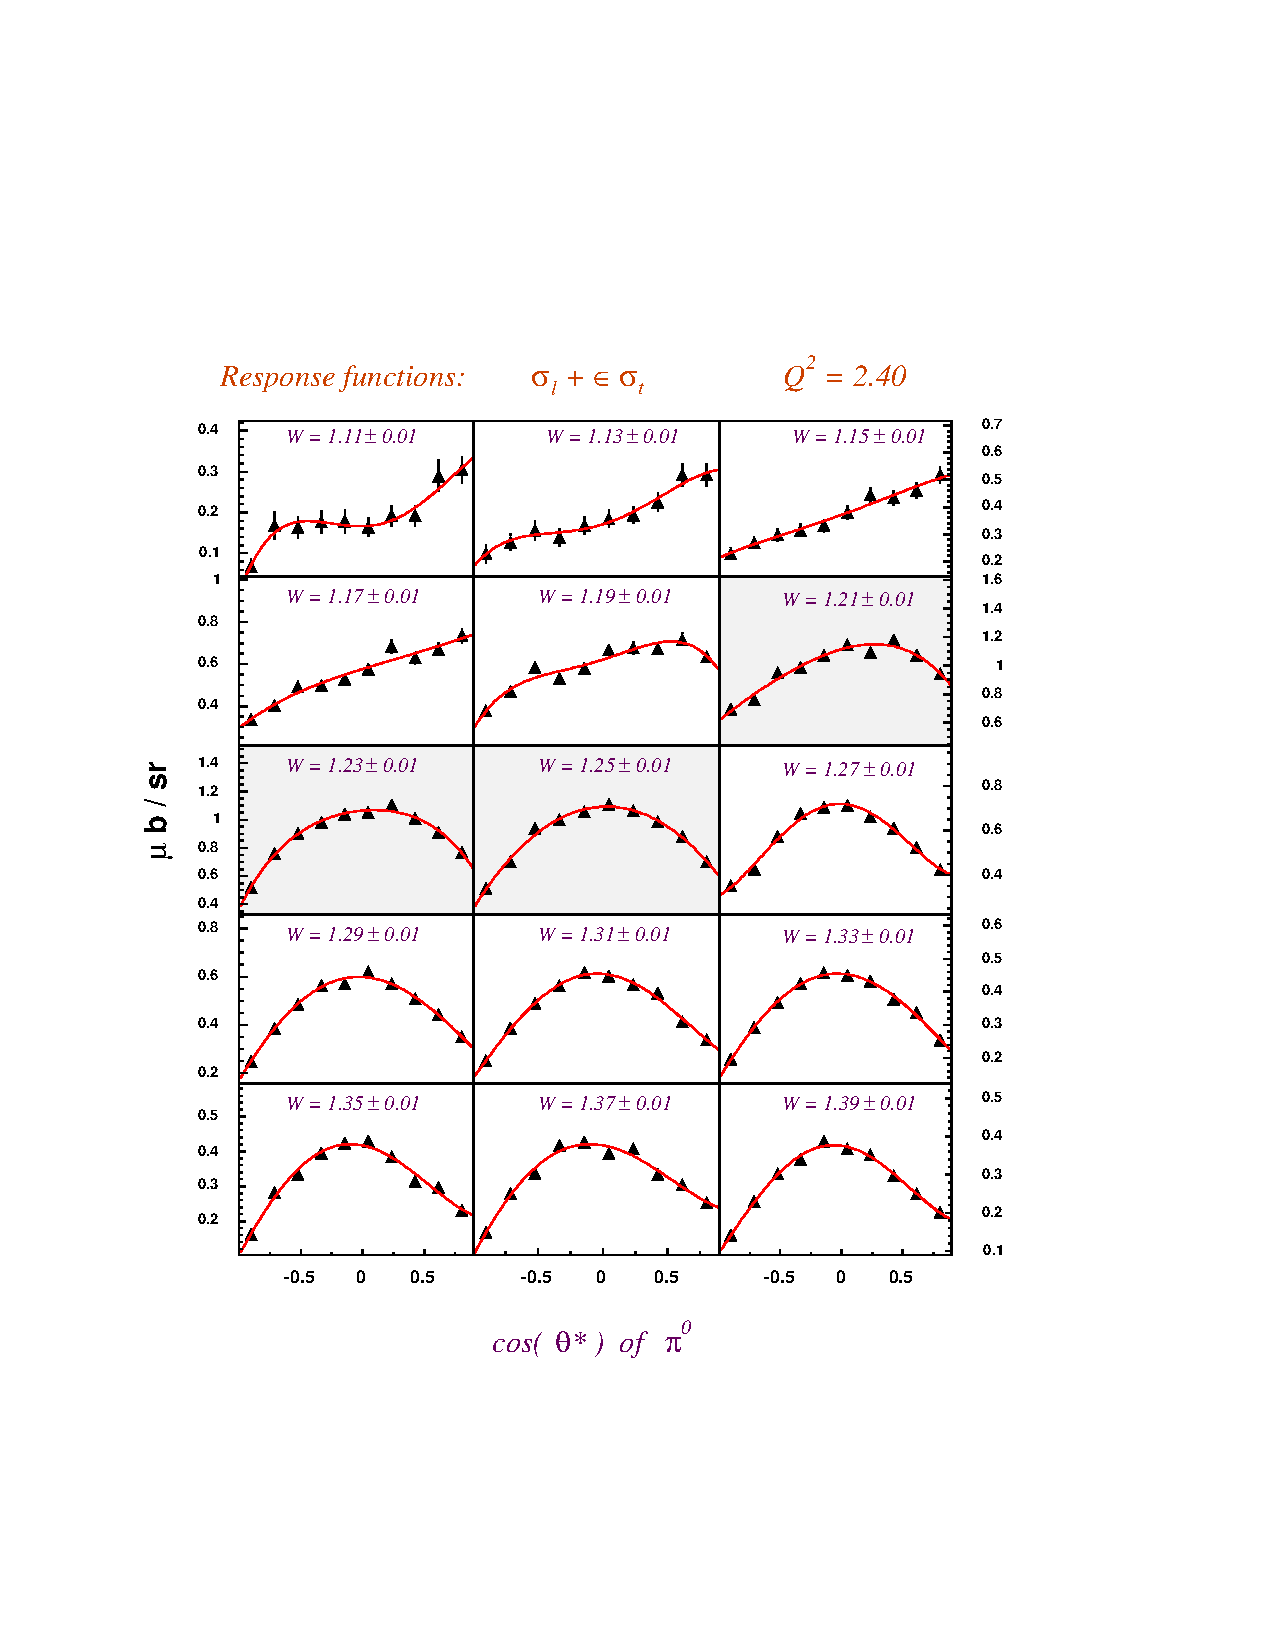
\includegraphics[width = 15cm, bb=0 100 500 640]{analysis/img/Sigma_lpt_Q2_2.40}
  \caption[$\sigma_L + \epsilon\sigma_T$ for different $W$ at $Q^2 = 2.4$ GeV$^2$]
          { $\sigma_L + \epsilon\sigma_T$ for different $W$ at $Q^2 = 2.4$ GeV$^2$. 
		     The legendre expansion (red line fit) is: 
		     $\sigma_T + \epsilon\sigma_L = A_0 + A_1P_1(cos\theta) + A_2P_2(cos\theta) 
		                                        + A_2P_3(cos\theta) + A_3P_4(cos\theta)$.\\
                     Regions near the $\Delta $ region are shaded.}
 \label{fig:Sigma_lpt_Q2_2.40}
\end{figure}



\begin{figure}[h]
 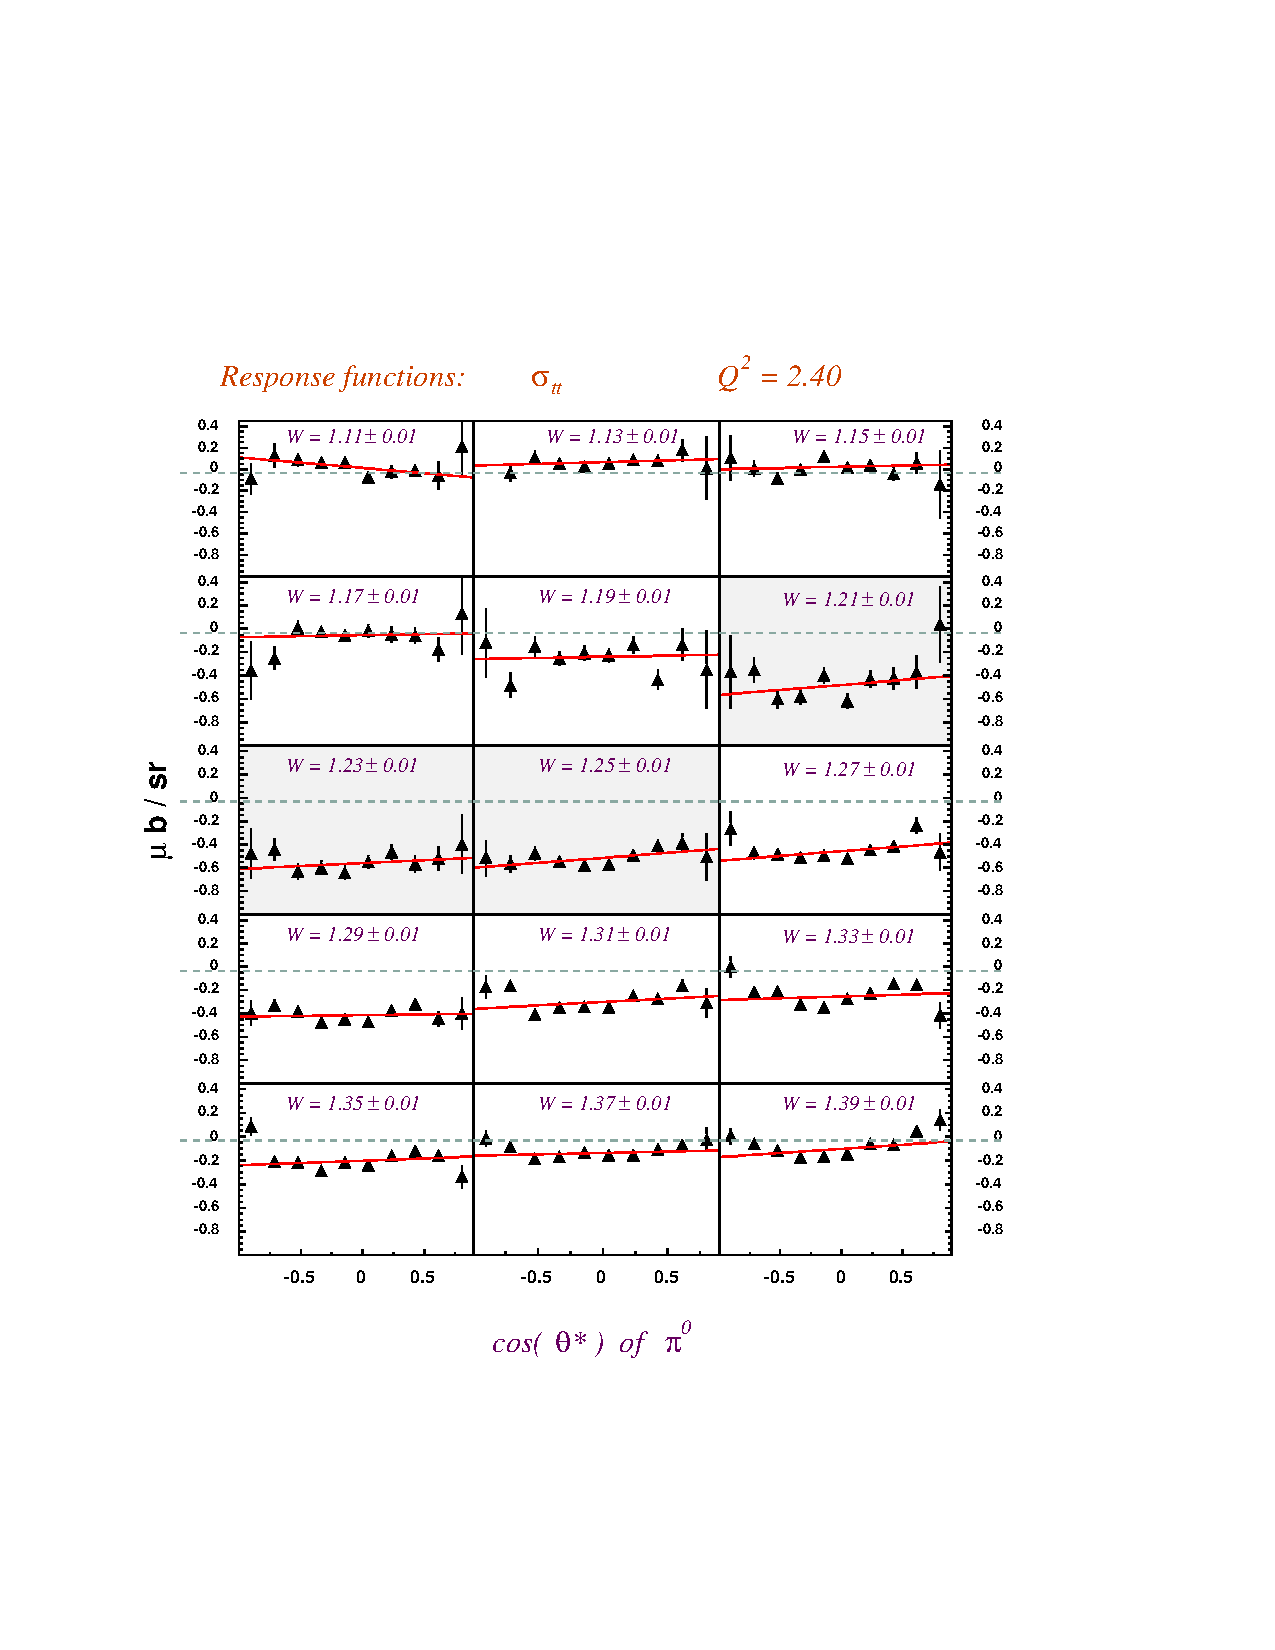
\includegraphics[width = 15cm, bb=0 100 500 640]{analysis/img/Sigma_tt_Q2_2.40}
  \caption[$\sigma_{TT}$ for different $W$ at $Q^2 = 2.4$ GeV$^2$]
          { $\sigma_{TT}$ for different $W$ at $Q^2 = 2.4$ GeV$^2$. 
		     The legendre expansion (red line fit) is: 
		     $\sigma_{TT} = C_0 + C_1P_1(cos\theta)$.	  \\
	             Regions near the $\Delta $ region are shaded.}
 \label{fig:Sigma_tt_Q2_2.40}
\end{figure}


\begin{figure}[h]
 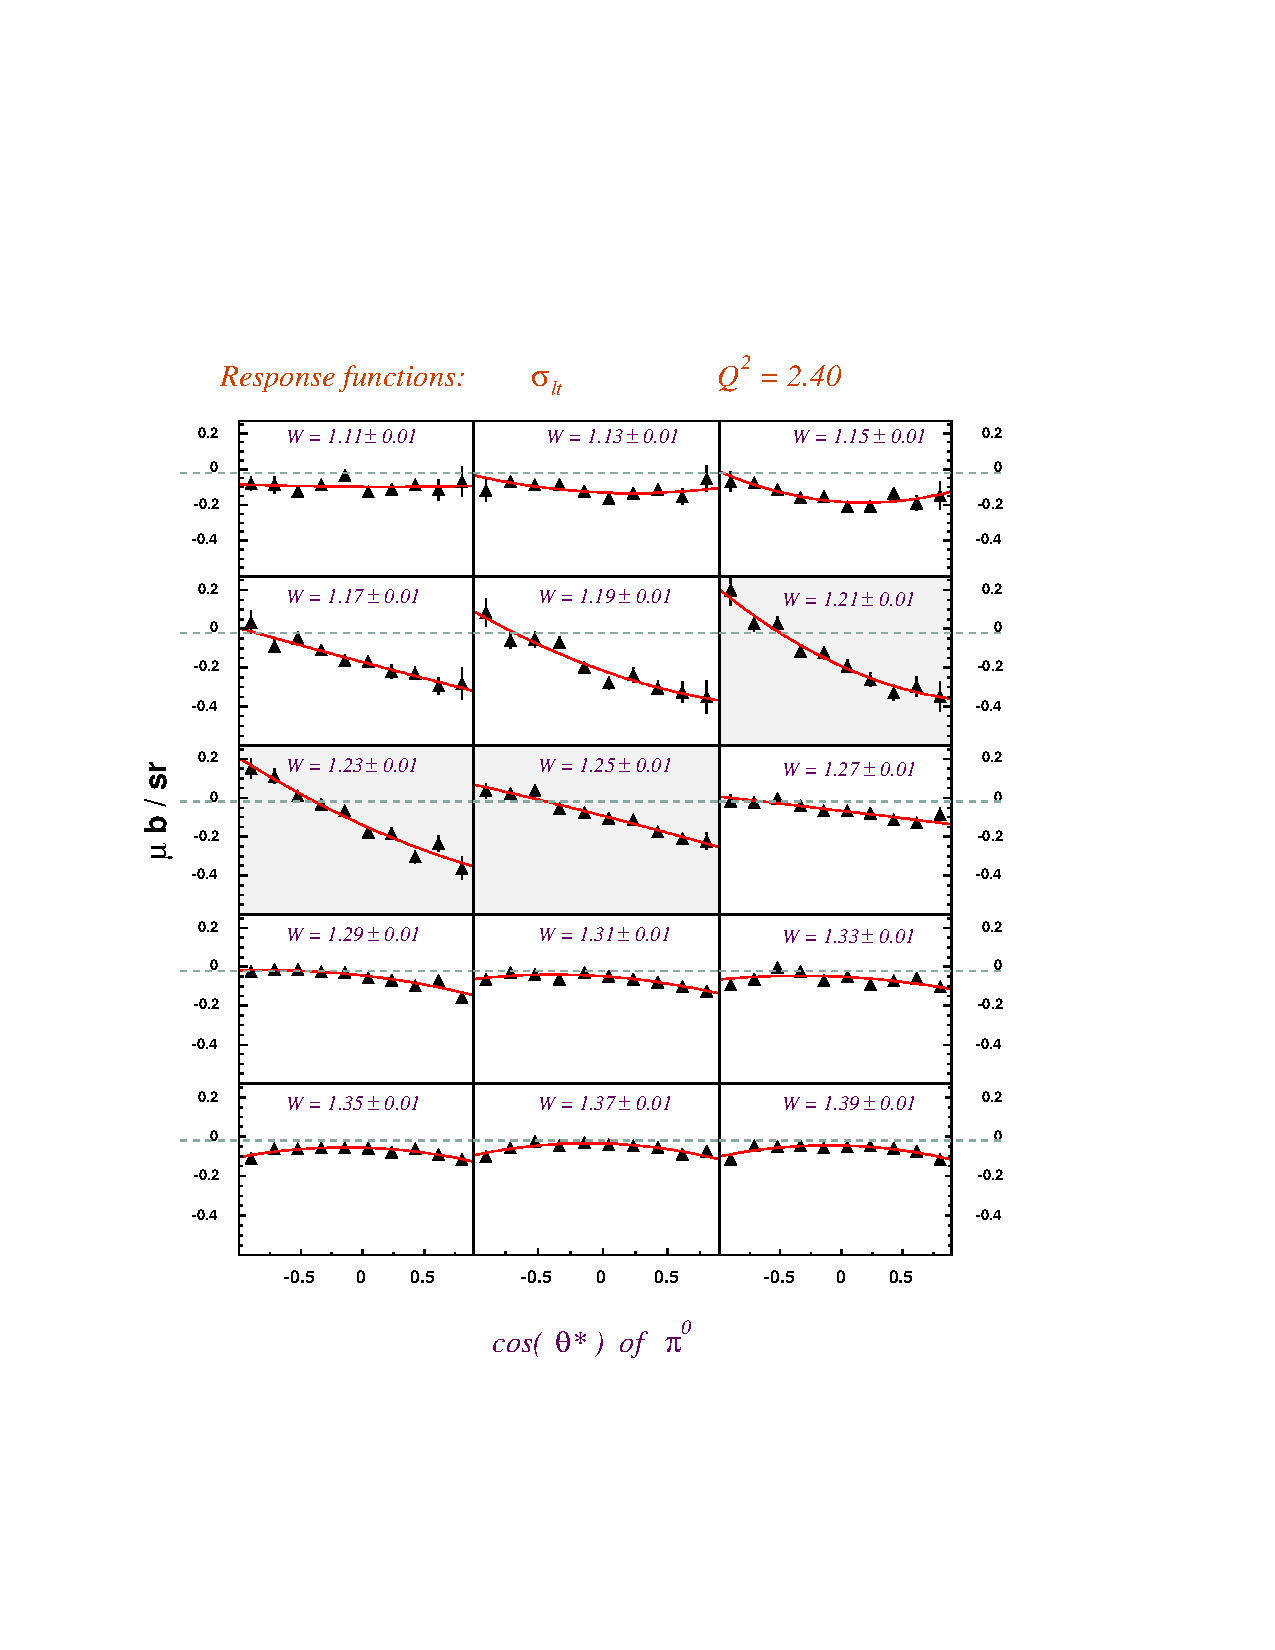
\includegraphics[width = 15cm, bb=0 100 500 640]{analysis/img/Sigma_lt_Q2_2.40}
  \caption[$\sigma_{LT}$ for different $W$ at $Q^2 = 2.4$ GeV$^2$]
          { $\sigma_{LT}$ for different $W$ at $Q^2 = 2.4$ GeV$^2$. 
		     The legendre expansion (red line fit) is: 
		     $\sigma_{LT} = D_0 + D_1P_1(cos\theta) + D_2P_2(cos\theta) $.\\
	             Regions near the $\Delta $ region are shaded.}
 \label{fig:Sigma_lt_Q2_2.40}
\end{figure}

\begin{figure}[h]
 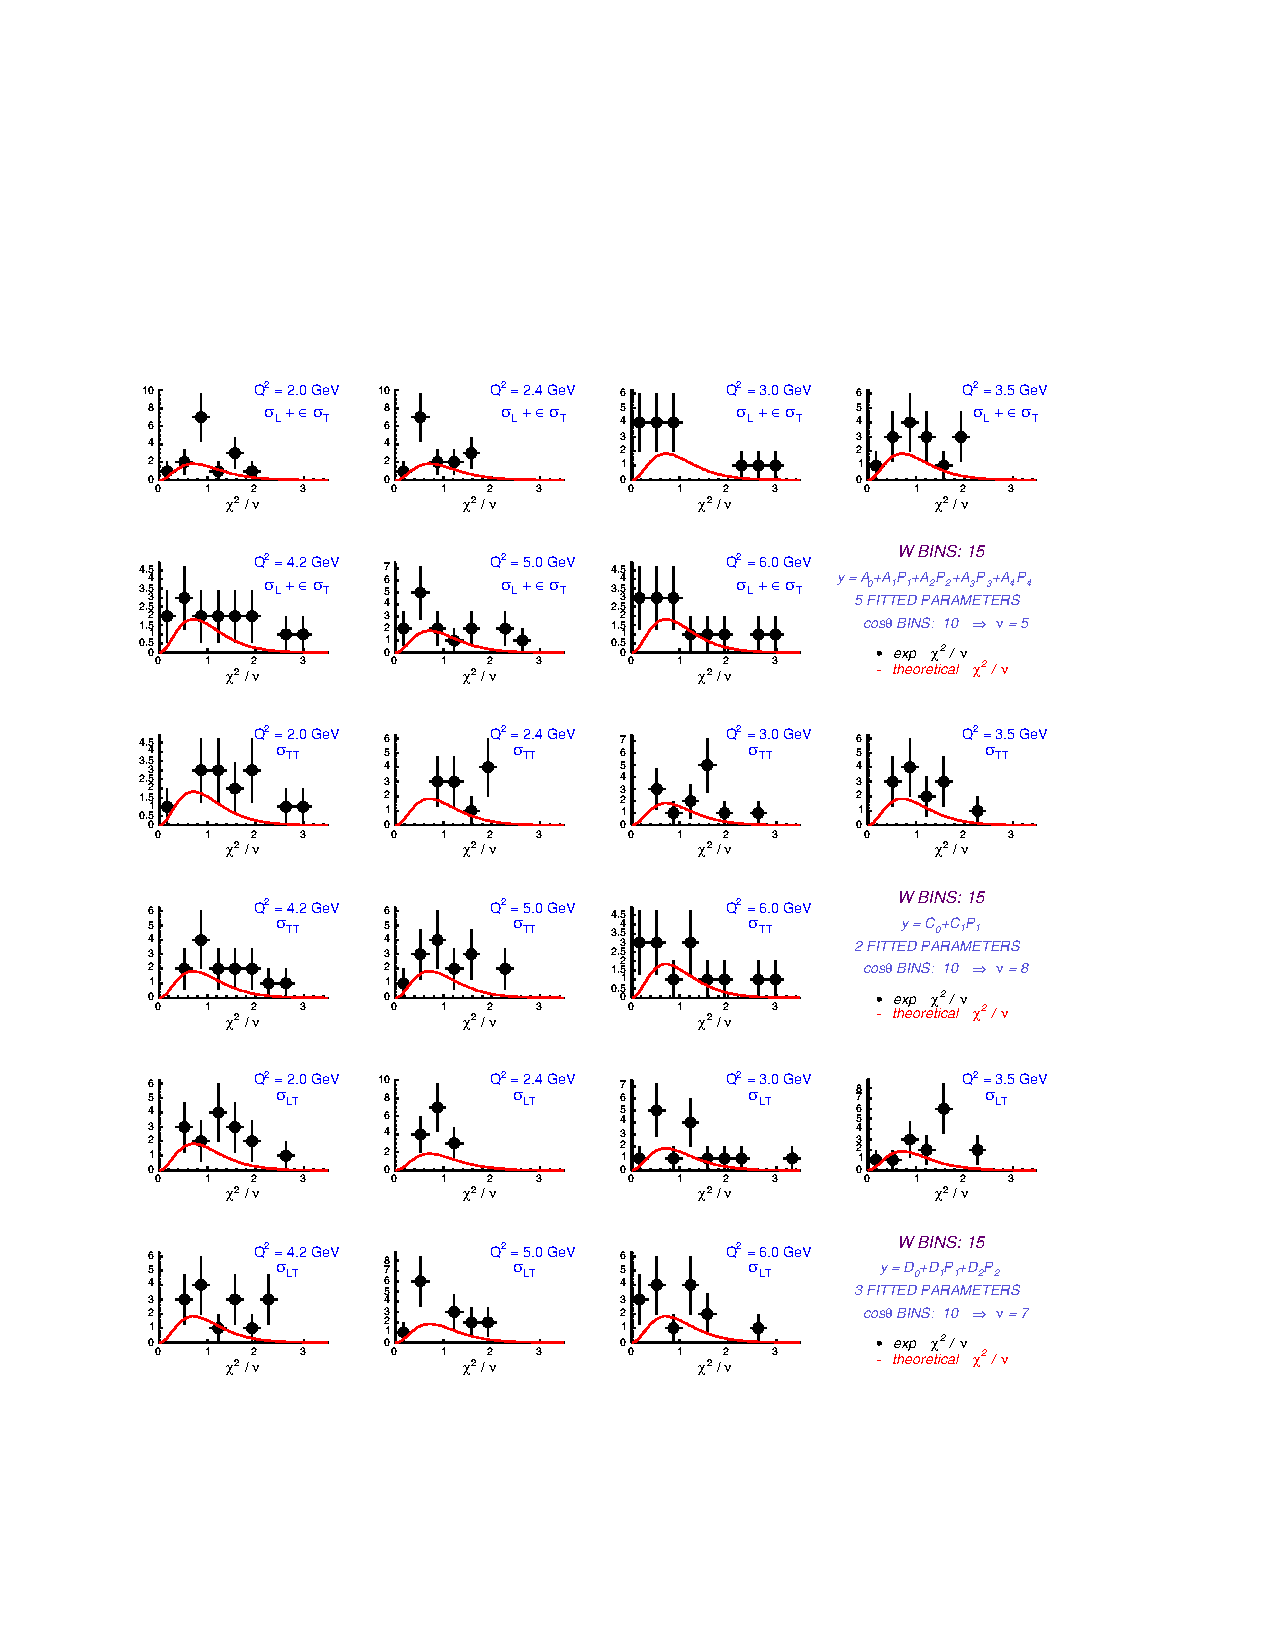
\includegraphics[width = 15.4cm, bb=40 100 530 640]{analysis/img/chi2_rtm} 
  \caption[Reduced $\chi^2$ distribution of the Legendre fits]
          { Reduced $\chi^2$ distribution of the Legendre fits. 
	             The $\sigma_L + \epsilon\sigma_T$, $\sigma_{TT}$ and  $\sigma_{LT}$ have respectively
		     5, 8, and 7 degrees of freedom. Each plot has only 15 points (there are 15 $W$ bins)
		     so the statistic of the $\chi^2/\nu $ distributions is poor. The red line is the expected 
		     $\chi^2$ distribution.}
 \label{fig:chi2_rtm}
\end{figure}

\cia
\F{fig:Coefficients_q2.4} shows the coefficients of the Legendre expansion for $Q^2=2.4$ GeV$^2$.
The coefficient $A_0 $, proportional to $M_{1+}$ if $\sigma_L << \sigma_T$ (see Eqn \ref{eqno:m1dominance}) and to the total c.m. cross section, 
shows the characteristic
resonance behaviour at the peak of the $\Delta$.


\begin{figure}[h]
 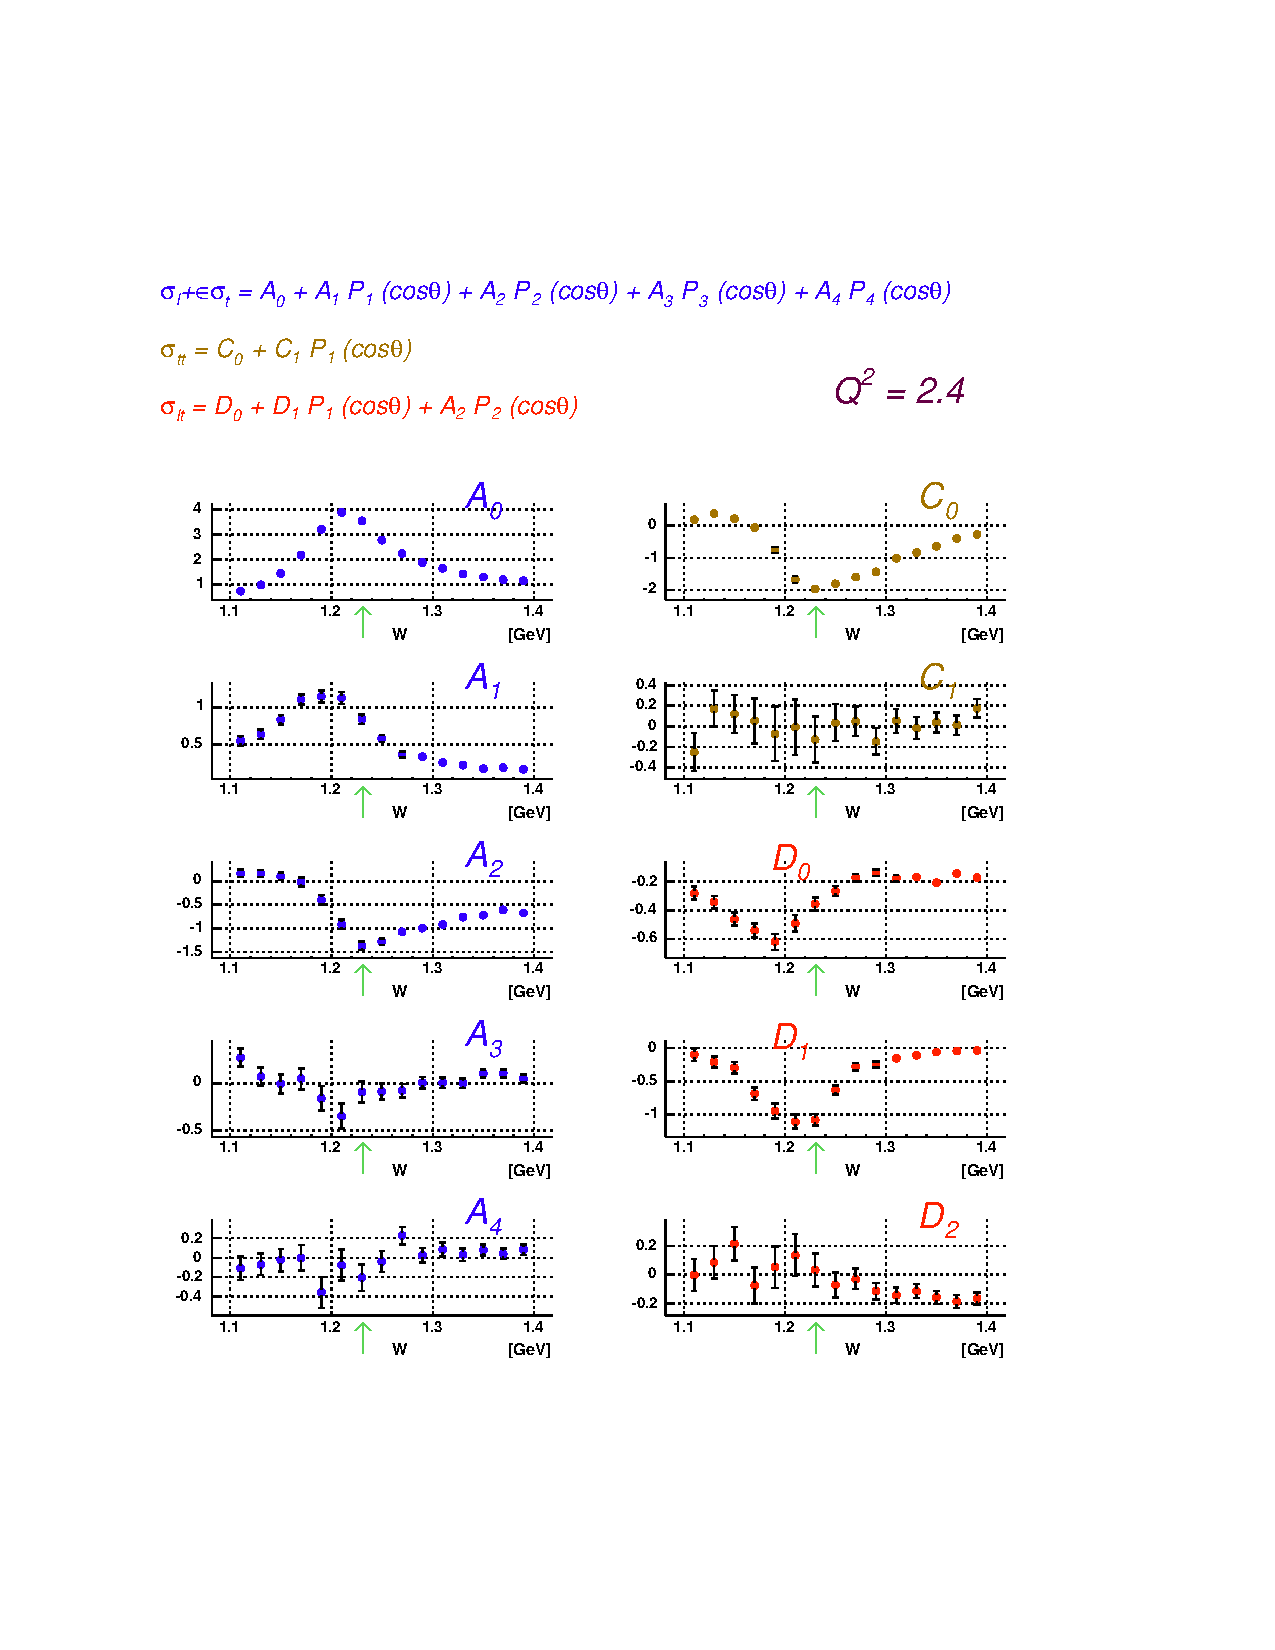
\includegraphics[width = 15cm, bb=0 100 540 700]{analysis/img/Coefficients_q2.4}
  \caption[Legendre coefficients at $Q^2 = 2.4$ GeV$^2$]
          { Legendre coefficients at $Q^2 = 2.4$ GeV$^2$. The green arrow shows the $\Delta$ mass
	             position. The coefficient $A_0$ is proportional to $M_{1+}$ and to the total c.m. cross section.}
 \label{fig:Coefficients_q2.4}
\end{figure}  


\cia
See    \begin{verbatim} 
http://www.jlab.org/~ungaro/pi0eprod/coefficients
\end{verbatim}
for the plots of the various coefficients for different cuts used in the analysis.

















\subsection{The $M_{1+}$ dominance assumption}
The approximation made  of $\ell$ up to d-waves
is a good approximation: one can see from \F{fig:Coefficients_q2.4}
that $A_4$, $C_1$, $D_2$ are rather small around the $\Delta$ compared to their
respectives coefficients with smaller $\ell$.
In order to make a model independent extraction of the multipoles a further approximation is needed.


Previous measurements at lower $Q^2$ showed that $E_{1+}$ and $S_{1+}$ are relatively small compared
to $M_{1+}$. All models that apply in this range of $Q^2$ show 
that $M_{1+}$ is the multipole that has the greatest strength.

The $M_{1+}$ dominance approximation consists in considering only  the multipoles
that interfere with $M_{1+}$.
With this approximation the relation between the Legendre coefficients and the electromagnetic multipoles
is \cite{bib:raskin}:
\begin{equation}
\begin{array}{l c l}
| M_{1+} |^2 & = & A_0/2 \\
Re(E_{1+}M_{1+}^*) & = & (A_2 - 2C_0/3)/8 \\
Re(S_{1+}M_{1+}^*) & = & D_1/6 \\
Re(E_{0+}M_{1+}^*) & = & A_1/2 \\
Re(S_{0+}M_{1+}^*) & = & D_0 \\
Re(M_{1-}M_{1+}^*) & = & -(A_2+2(A_0+C_0))/8 \\
\end{array}
\label{eqno:m1dominance}
\end{equation}

To obtain the various multipole ratios $\Re_{m}$ at the resonance peak, a Taylor expansion 
distribution around $M_W = 1.232$ $GeV$ is performed, as shown in \F{fig:multiem_taylor} \F{fig:multism_taylor}:
$$
\Re_{m} (W) \sim a_0 + a_1(x-M_W) + a_2(x-M_W)^2 + ...  = \sum_{i}a_i(x-M_W)^i
$$
with this expansion, at the $\Delta $ peak we have $\Re_{m} = a_0$.

\begin{figure}[h]
 \begin{center}
 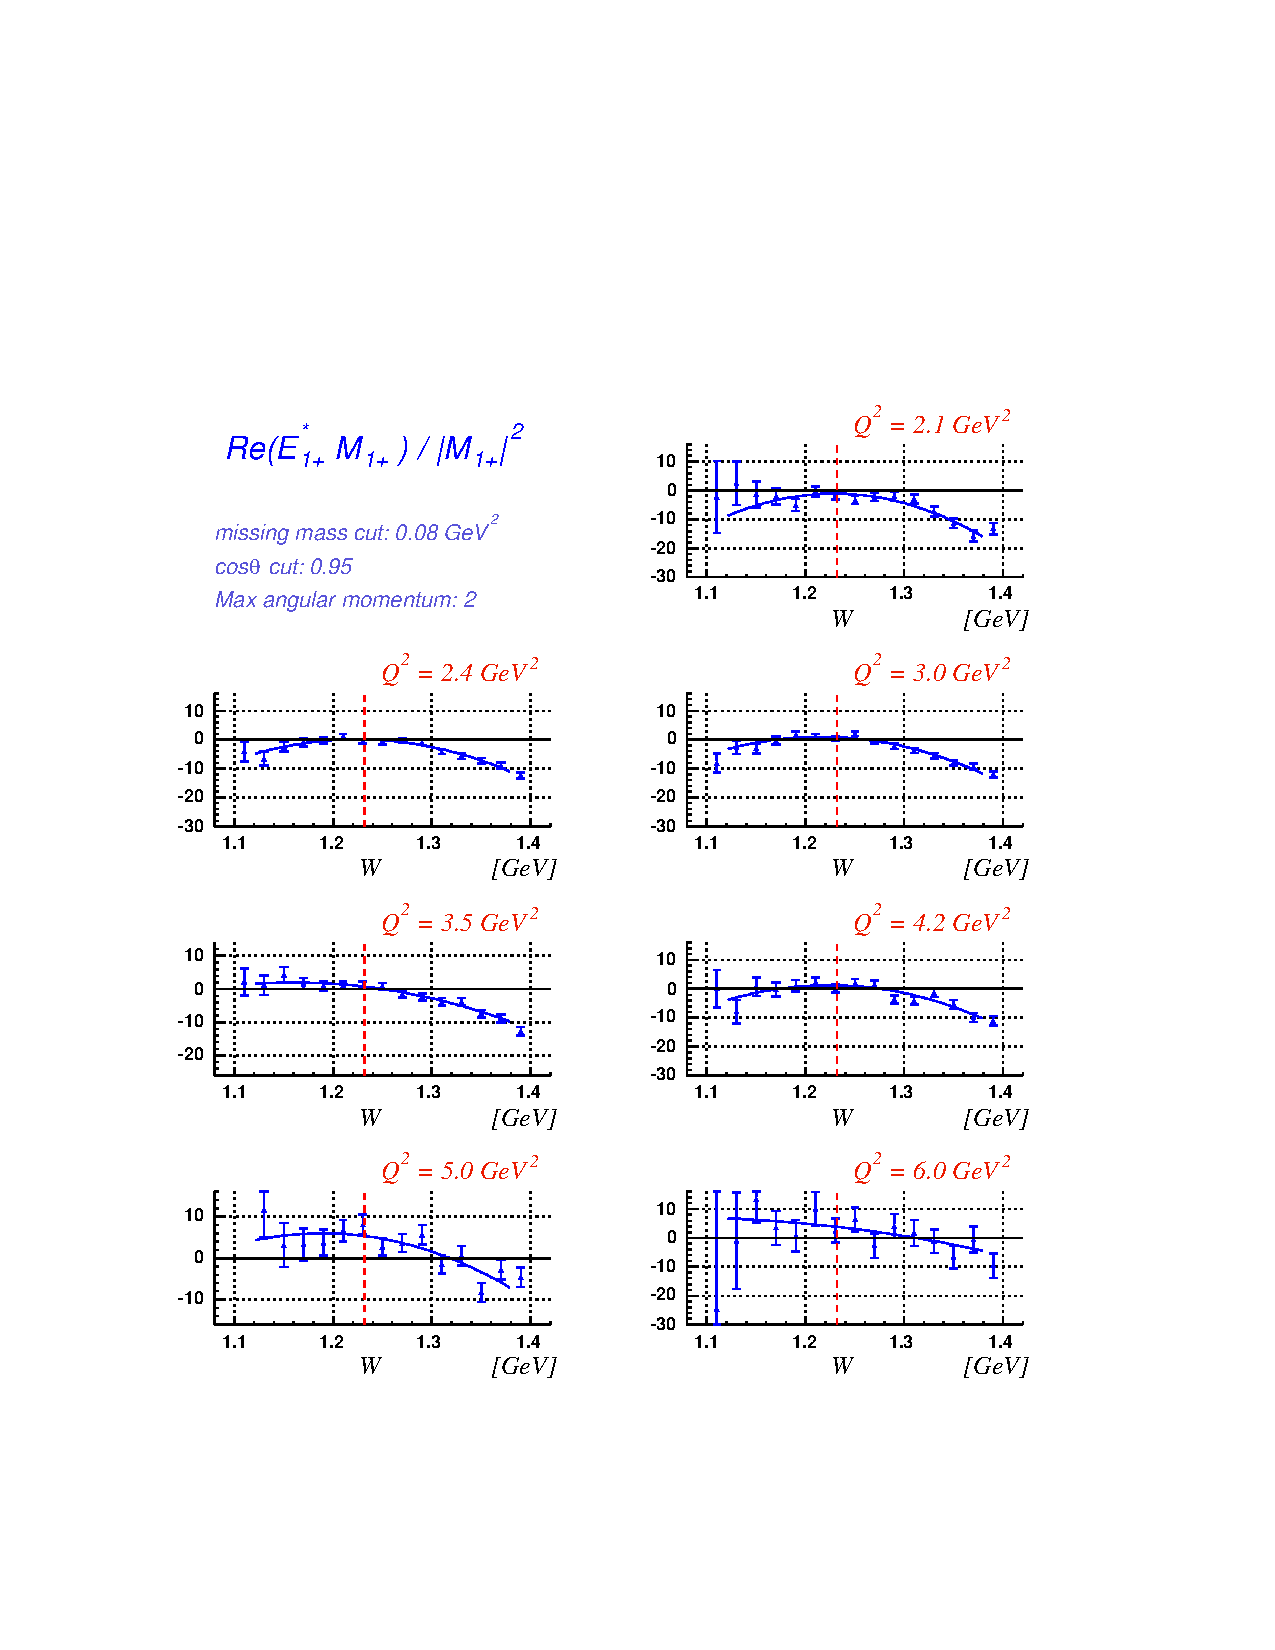
\includegraphics[width = 13cm, bb=30 130 550 600]{analysis/img/multiem_taylor} 
  \caption[ $Re(E_{1+}M_{1+}^*)$ as a function of $W$ for different $Q^2$.]
{ $Re(E_{1+}M_{1+}^*)$ as a function of $W$ for different $Q^2$. The value at the $\Delta $ peak
is the $a_0$ coefficient of the Taylor expansion around $M_W = 1.232$}
 \label{fig:multiem_taylor}
 \end{center}
\end{figure}
\begin{figure}[h]
 \begin{center}
 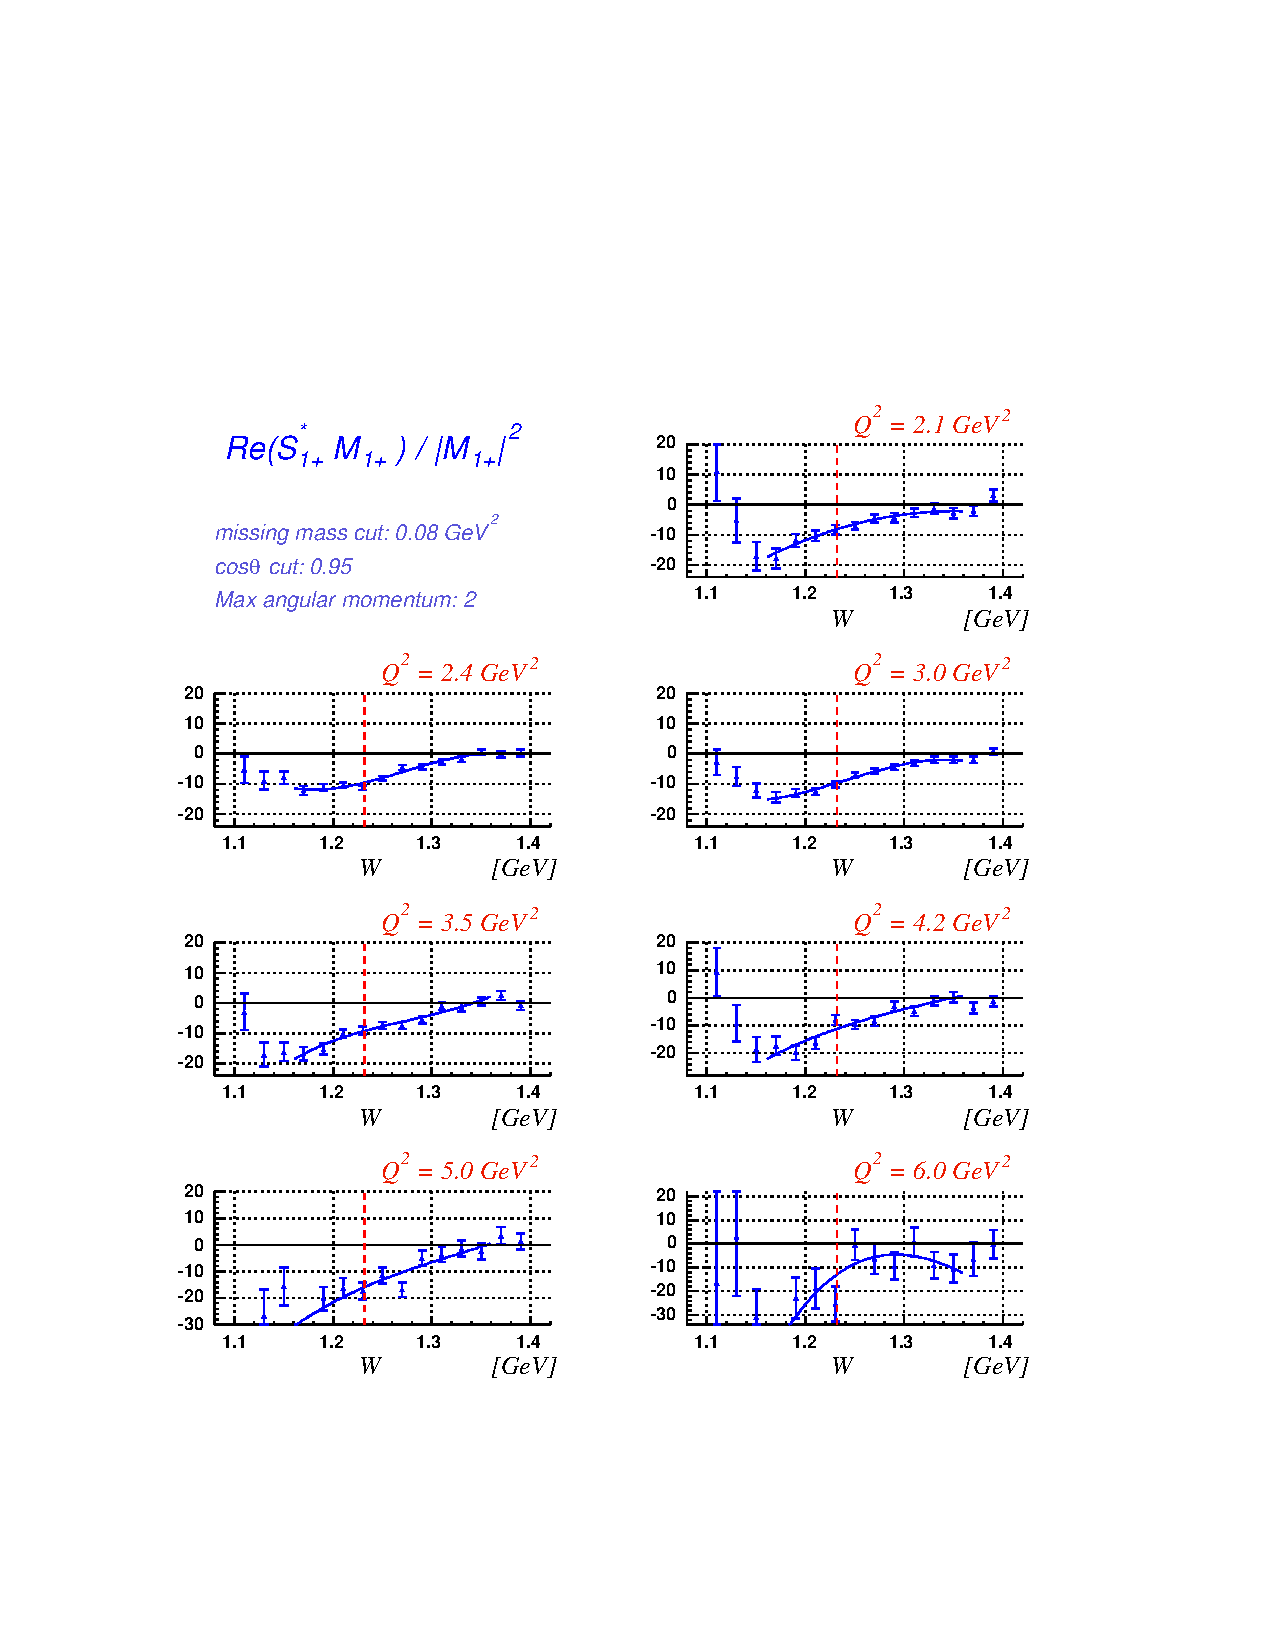
\includegraphics[width = 13cm, bb=30 130 550 600]{analysis/img/multism_taylor} 
  \caption[ $Re(S_{1+}M_{1+}^*)$ as a function of $W$ for different $Q^2$.]
{ $Re(S_{1+}M_{1+}^*)$ as a function of $W$ for different $Q^2$. The value at the $\Delta $ peak
is the $a_0$ coefficient of the Taylor expansion around $M_W = 1.232$}
 \label{fig:multism_taylor}
 \end{center}
\end{figure}
To see all the multipoles and multipoles ratios plots see
\begin{verbatim} 
http://www.jlab.org/~ungaro/pi0eprod/multipoles
\end{verbatim}



\subsection{ Effect of $M_{1+}$ dominance and $\ell \le 2$ approximation}
\label{sec:m1pdomeffect}
The $M_{1+}$ dominance assumption and
the limited order ($\ell \le 2$) in the Legendre expansion of the structure functions
introduce an uncertainty in the extraction of the multipoles which is expected to 
become greater with increasing $Q^2$.

In order to evaluate such uncertainty
two models (MAID, DMT) were used to generate the cross sections $\sigma_{MAID}$ and $\sigma_{DMT}$.
These models provide the multipoles $E_{\ell\pm}$, $S_{\ell\pm}$, $M_{\ell\pm}$ with $\ell$ up tp $5$.

The generated cross section were fitted as described in Section \ref{sec:structure} to extract
the structure functions. The structure functions were fitted
with orthogonal Legendre polynomials with $\ell$ up to d-waves as in Section \ref{sec:legendre}.
The approximation (\ref{eqno:m1dominance}) was used in order to extract the multipoles.

\F{fig:maid_comp} and \F{fig:dmt_comp} show the model and extracted multipole ratios for 
$Q^2$ = $3.5$ GeV$^2$.

One can see that in the $\Delta$ region DMT prescribes a smaller 
value of $S_{1+}$ then MAID.  The differences become even larger at higher $Q^2$.
$E_{1+}$ remains negative and constant for MAID while it becomes positive in DMT between $Q^2$ of $3$ and $4$
GeV$^2$.
\begin{figure}[h]
 \begin{center}
 \includegraphics[width = 15cm, bb=30 130 500 600]{analysis/img/multipoles_q2_3.5_data1}
  \caption[Comparison between the model (dashed blue line) and extracted (red points) multipole ratios for MAID 2000]
          { Comparison between the model and extracted multipole ratios for MAID 2000 at $Q^2$ = $3.5$ GeV$^2$.}
 \label{fig:maid_comp}
 \end{center}
\end{figure}

\begin{figure}[h]
 \begin{center}
 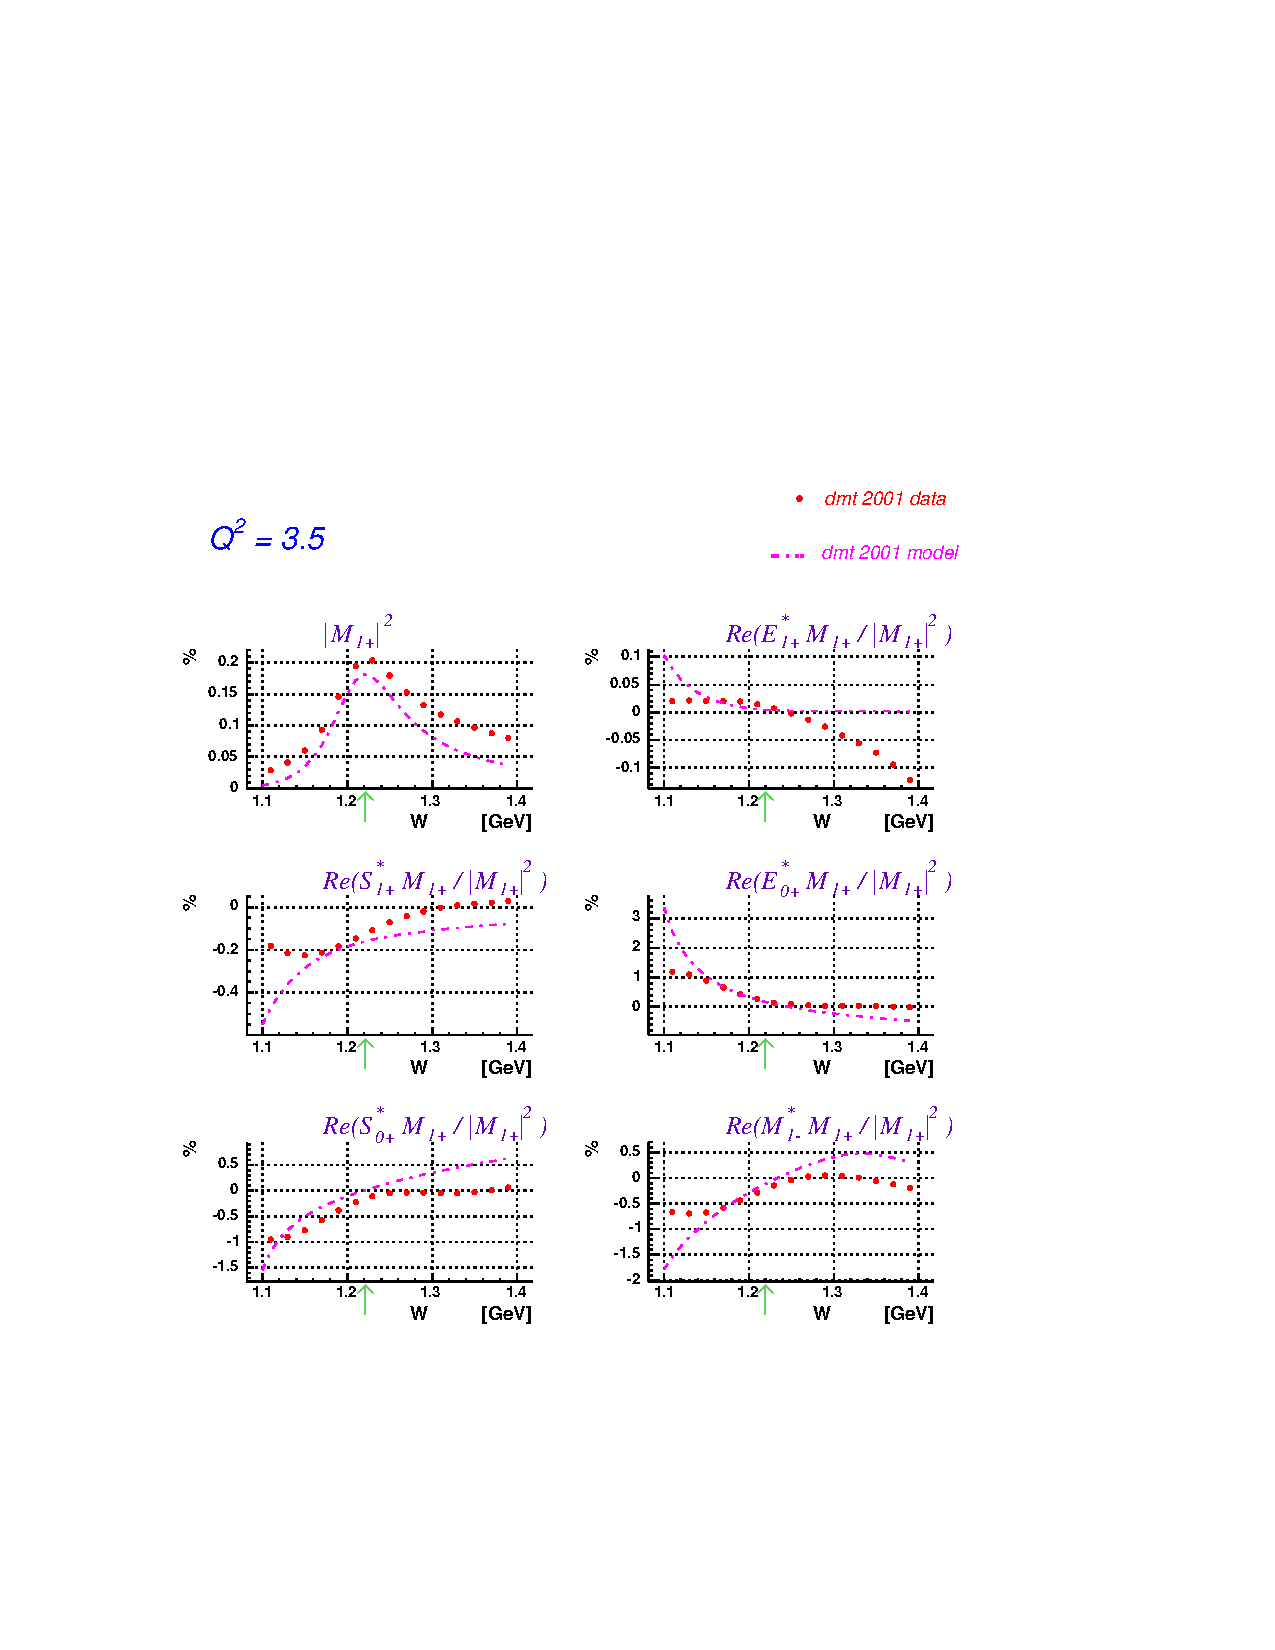
\includegraphics[width = 15cm, bb=60 100 540 600]{analysis/img/multipoles_q2_3.5_data2}
  \caption[Comparison between the model (dashed blue line) and extracted (red points) multipole ratios for DMT 2001]
          { Comparison between the model and extracted multipole ratios for DMT 2001 at $Q^2$ = $3.5$ GeV$^2$. }
 \label{fig:dmt_comp}
\end{center}
\end{figure}

\cia
The difference between the extracted multipole with the
model prediction at the $\Delta$ peak is illustrated in \F{fig:error_rm} for $E_{1+}/M_{1+}$ and in \F{fig:error_rs} for $S_{1+}/M_{1+}$.
\begin{figure}[h]
 \begin{center}
 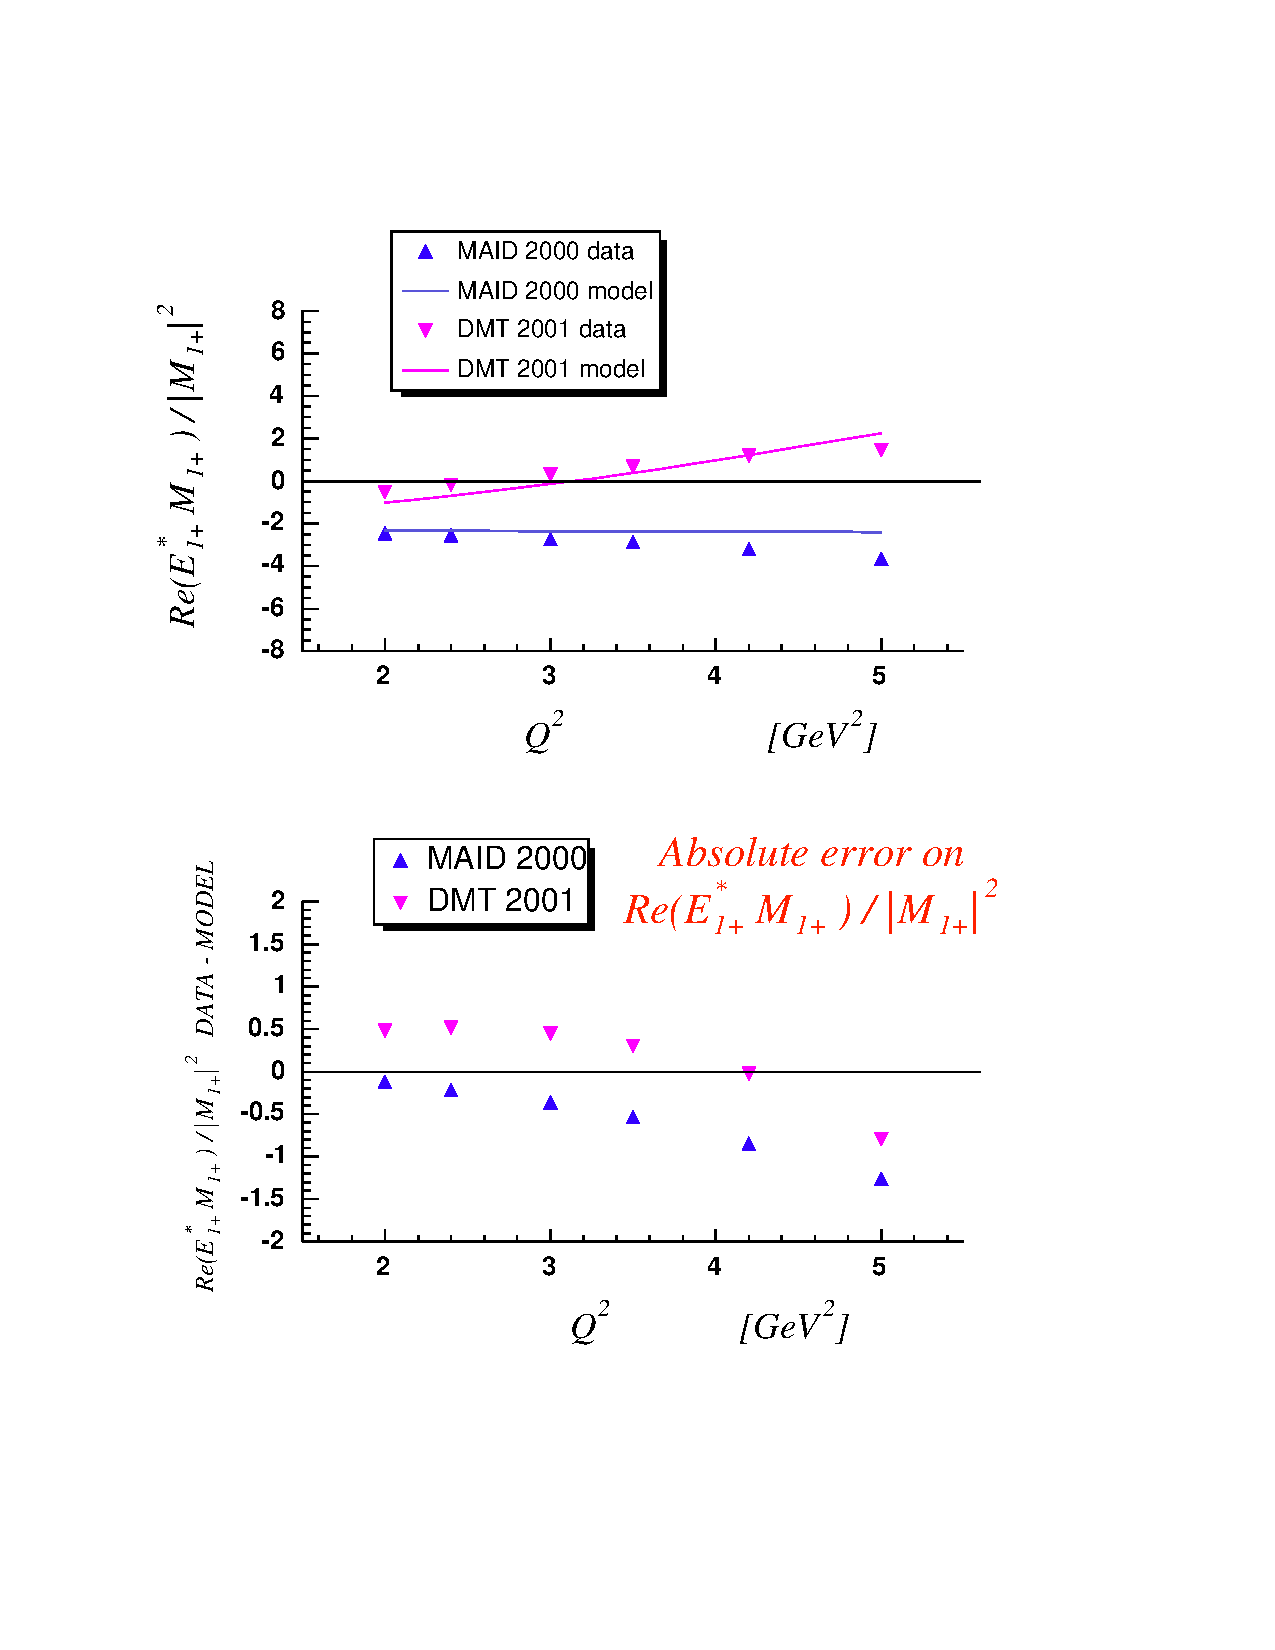
\includegraphics[width = 12cm, bb=30 130 560 720]{analysis/img/error_rm} 
  \caption[Model and extracted $E_{1+}/M_{1+}$ as a function of $Q^2$]
          {  Model and $M_{1+}$ dominance extracted $E_{1+}/M_{1+}$ as a function of $Q^2$. Top: 
	              the points are the value from the fit and the approximations described in
		      the text. The lines
		      are the model prediction. Bottom: absolute difference between between
		      extracted value and model prediction.}
 \label{fig:error_rm}
\end{center}
\end{figure}

When MAID is used the ratio $E_{1+}/M_{1+}$ is always underestimated, starting
at $\sim 0.2\%$ at $Q^2=2$ GeV$^2$ and up to $\sim 1.2\%$ at $Q^2=5$ GeV$^2$.
When DMT is used a rather constant overestimation by $\sim 0.5\%$ of $E_{1+}/M_{1+}$ up to $Q^2=3.5$ GeV$^2$ is obtained.
At $Q^2=4.2$ the value extracted is the same as in the model but at $Q^2=5$ $E_{1+}/M_{1+}$ is underestimated
by $\sim 0.8\%$.

As regarding $S_{1+}/M_{1+}$, the extraction from both models yelds a rather significant overestimation 
increasing in value with $Q^2$.
 
\begin{figure}[h]
 \begin{center}
 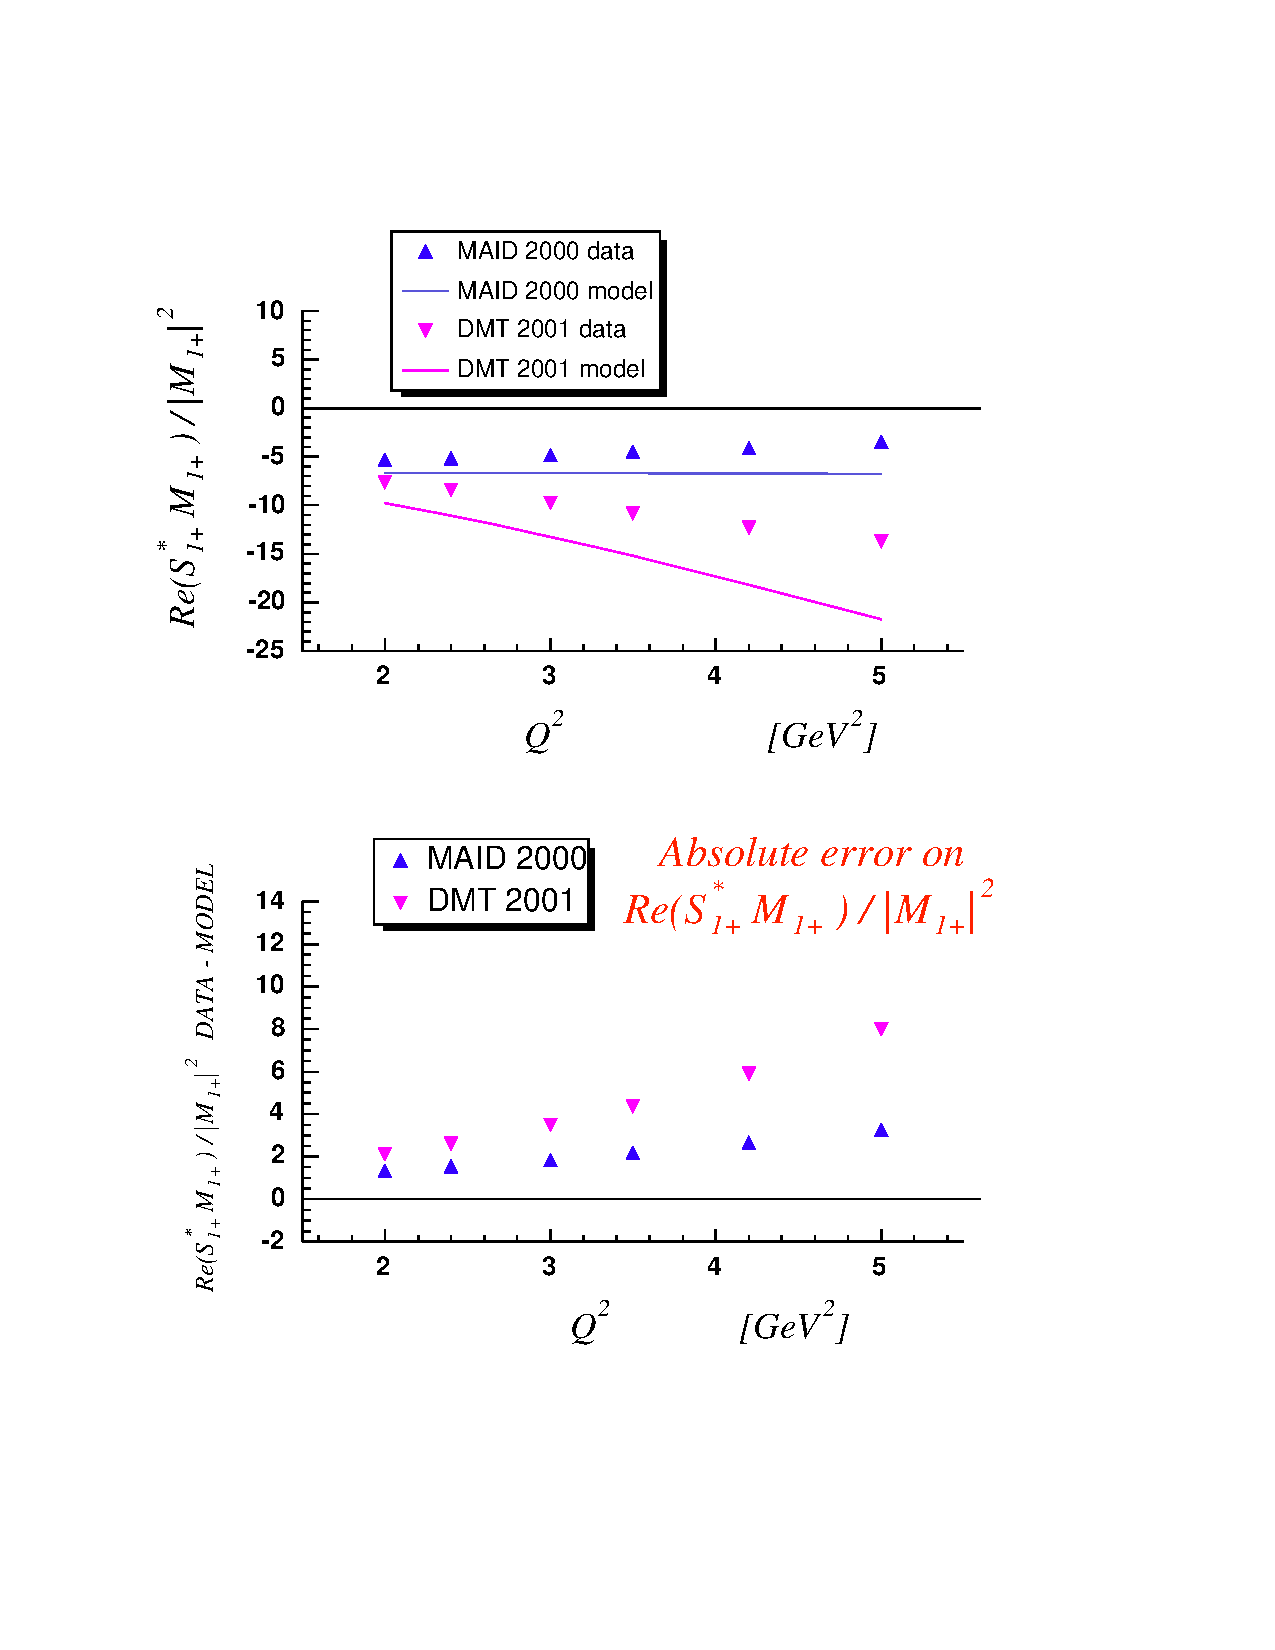
\includegraphics[width = 12cm, bb=30 130 560 720]{analysis/img/error_rs} 
  \caption[Model and extracted $S_{1+}/M_{1+}$ as a function of $Q^2$]
          {  Model and $M_{1+}$ dominance extracted $S_{1+}/M_{1+}$ as a function of $Q^2$. Top: 
	              the points are the value from the fit and the approximations described in
		      the text. The lines
		      are the model prediction. Bottom: absolute difference between between
		      extracted value and model prediction.}
 \label{fig:error_rs}
\end{center}
\end{figure}



















\cia
\subsection{Multipole Truncation Results for $R_{EM}$ and $R_{SM}$}
The result for the ratios $R_{EM}$ and $R_{SM}$ are shown in Table 
\ref{tab:result_ratio} for different values of $Q^2$.

The fits suggest a zero crossing for $R_{EM}$ between $Q^2$ of $3.0$ and $4.0$ GeV$^2$.

\begin{table}[h]
 \begin{center}
  \begin{tabular}{c | c | c}
          & & \\
    \hline\hline    
        & & \\
    $Q^2$ (GeV$^2$)&     $R_{EM}$ ($\%, E_{STAT},E_{SYS}$)   &    $R_{SM}$ ($\%, E_{STAT},E_{SYS}$) \\ 
    & & \\
    \hline\hline
        & & \\

     
2.15  & $  -1.0 \pm 0.7 \pm 0.05  $  &  $ -10.0  \pm 0.9 \pm 0.06 $ \\
2.4   & $  0.4  \pm 0.3 \pm 0.2   $  &  $ -11.7  \pm 0.5 \pm 0.2  $ \\
3     & $  1.3  \pm 0.4 \pm 0.3   $  &  $ -12.5  \pm 0.5 \pm 0.07 $ \\
3.5   & $  1.2  \pm 0.5 \pm 0.3   $  &  $ -12.9  \pm 0.7 \pm 0.2  $ \\
4.2   & $  1.7  \pm 0.6 \pm 0.4   $  &  $ -17.3  \pm 1.0 \pm 0.14 $ \\
5     & $  6.0  \pm 1.0 \pm 0.5   $  &  $ -24.0  \pm 1.8 \pm 0.24 $ \\
6     & $  4.8  \pm 1.8 \pm 0.7   $  &  $ -24.0  \pm 4   \pm 0.4  $ \\
& & \\
    \hline
  \end{tabular}
 \end{center} 
 \caption{ Results for $R_{EM}$ and $R_{SM}$ in the multipole truncation analysis.}
 \label{tab:result_ratio}
\end{table}

$R_{EM}$ is shown in \F{fig:RM} along with the prediction from DMT 2001 and MAID 2000 models.
Previous data from CLAS and Hall C (using  $M_{1+}$ dominance and $\ell \le 1$ approximations) 
are also plotted.


\begin{figure}[h]
 \begin{center}
 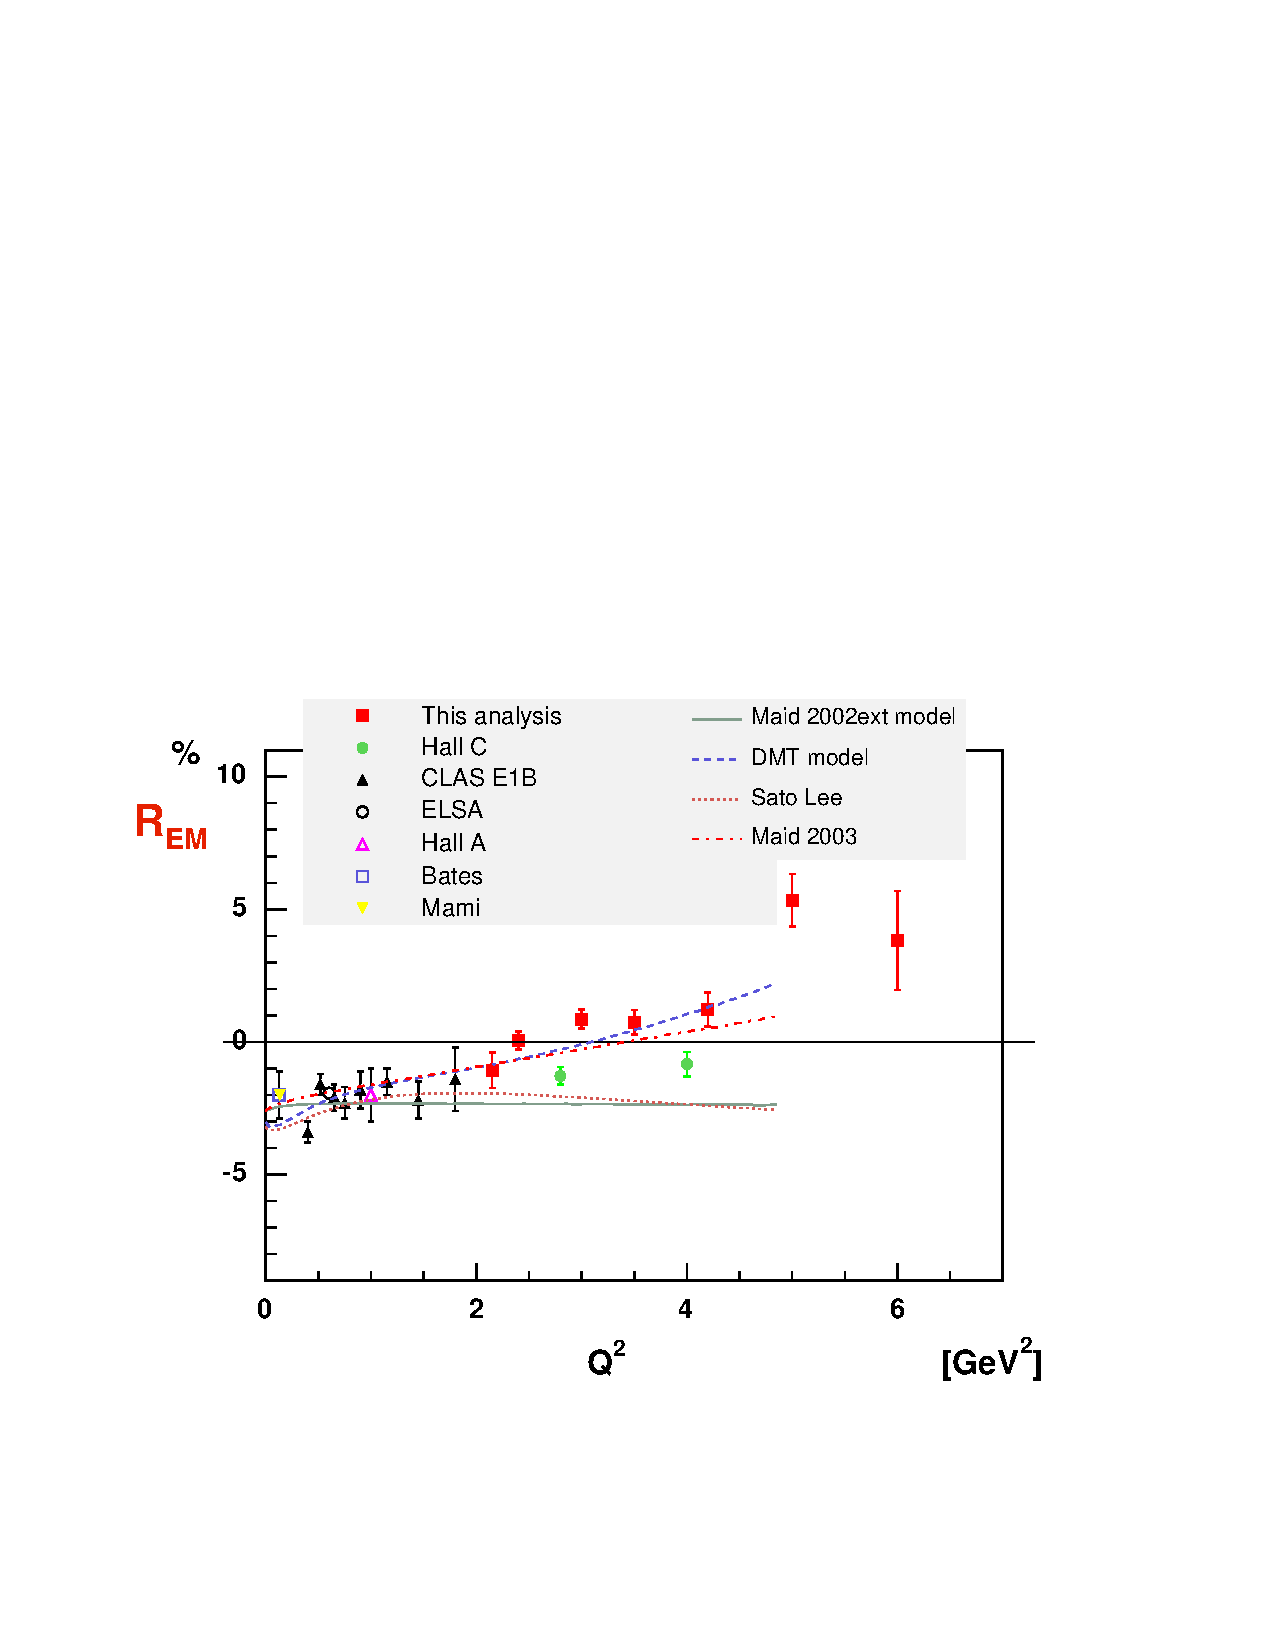
\includegraphics[width = 11cm, bb=30 130 520 500]{analysis/img/RM} 
  \caption[Result for $R_{EM}$ as a function of $Q^2$]
          {  Result for $R_{EM}$ as a function of $Q^2$ obtained in the $M_{1+}$ dominance approximation.}
 \label{fig:RM}
\end{center}
\end{figure}


\begin{figure}[h]
 \begin{center}
 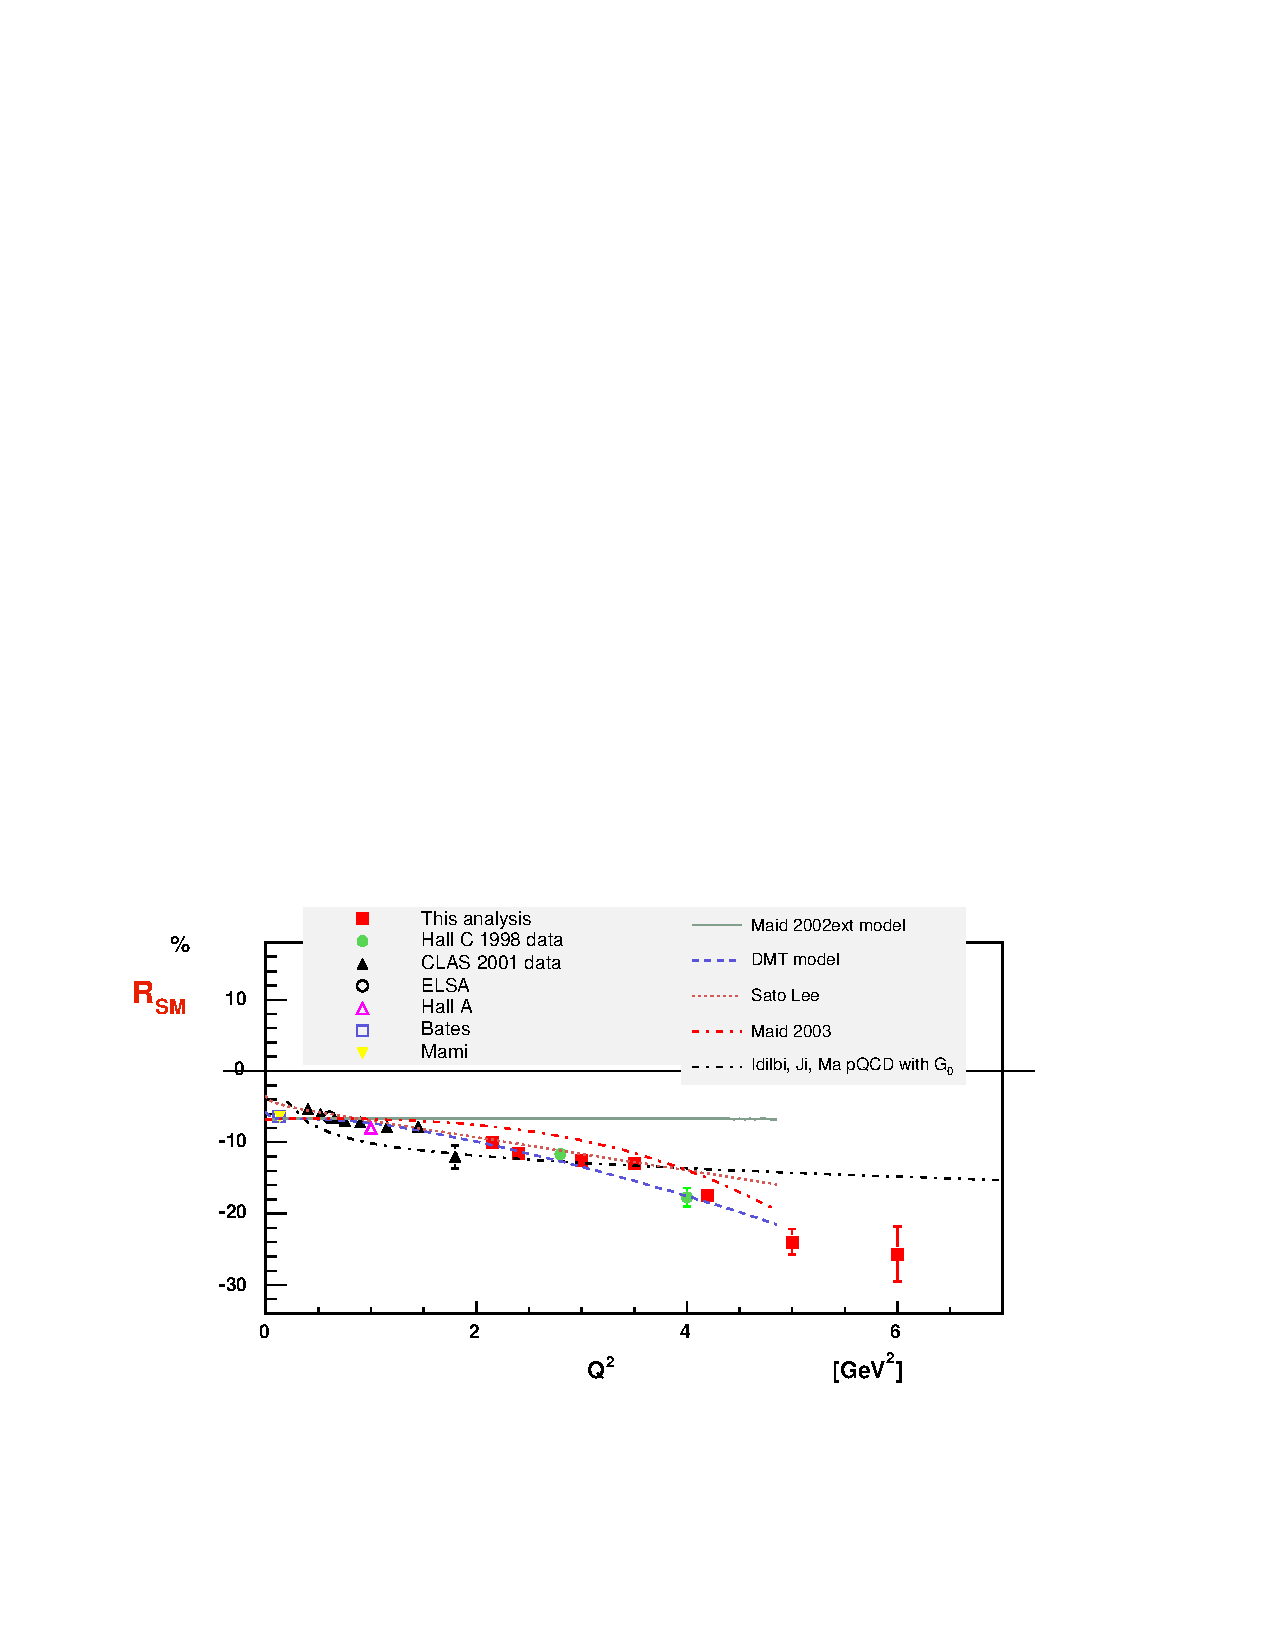
\includegraphics[width = 11cm, bb=30 130 520 500]{analysis/img/RS} 
  \caption[Result for $R_{SM}$ as a function of $Q^2$]
          {  Result for $R_{SM}$ as a function of $Q^2$ obtained in the $M_{1+}$ dominance approximation.}
 \label{fig:SM}
\end{center}
\end{figure}

\cia
\subsection{Amplitudes of $M_{1-}$, $E_{0+}$, $S_{0+}$}
Equations  (\ref{eqno:m1dominance}) holds if $|M_{1+}| >> |M_{\ell\pm}|$ where $ M_{\ell\pm}$ is any 
e.m. multipole that can contribute to the process. The extraction of $M_{1-}$, $E_{0+}$ and $S_{0+}$
using (\ref{eqno:m1dominance}) is a consistency check of the  $M_{1+}$ dominance assumption.
In \F{fig:M1m} and \F{fig:E0p} it is shown the result of the ratios  Re$(M_{1-}^*M_{1+})/|M_{1+}|^2$, 
Re$(E_{0+}^*M_{1+})/|M_{1+}|^2$ and Re$(S_{0+}^*M_{1+})/|M_{1+}|^2$. These amplitudes are 
about $10-20 \% $ of in $|M_{1+}|$ amplitude, increasing with $Q^2$. This rather large result suggest that   
Equations  (\ref{eqno:m1dominance}) are only approximate.

\begin{figure}[h]
 \begin{center}
 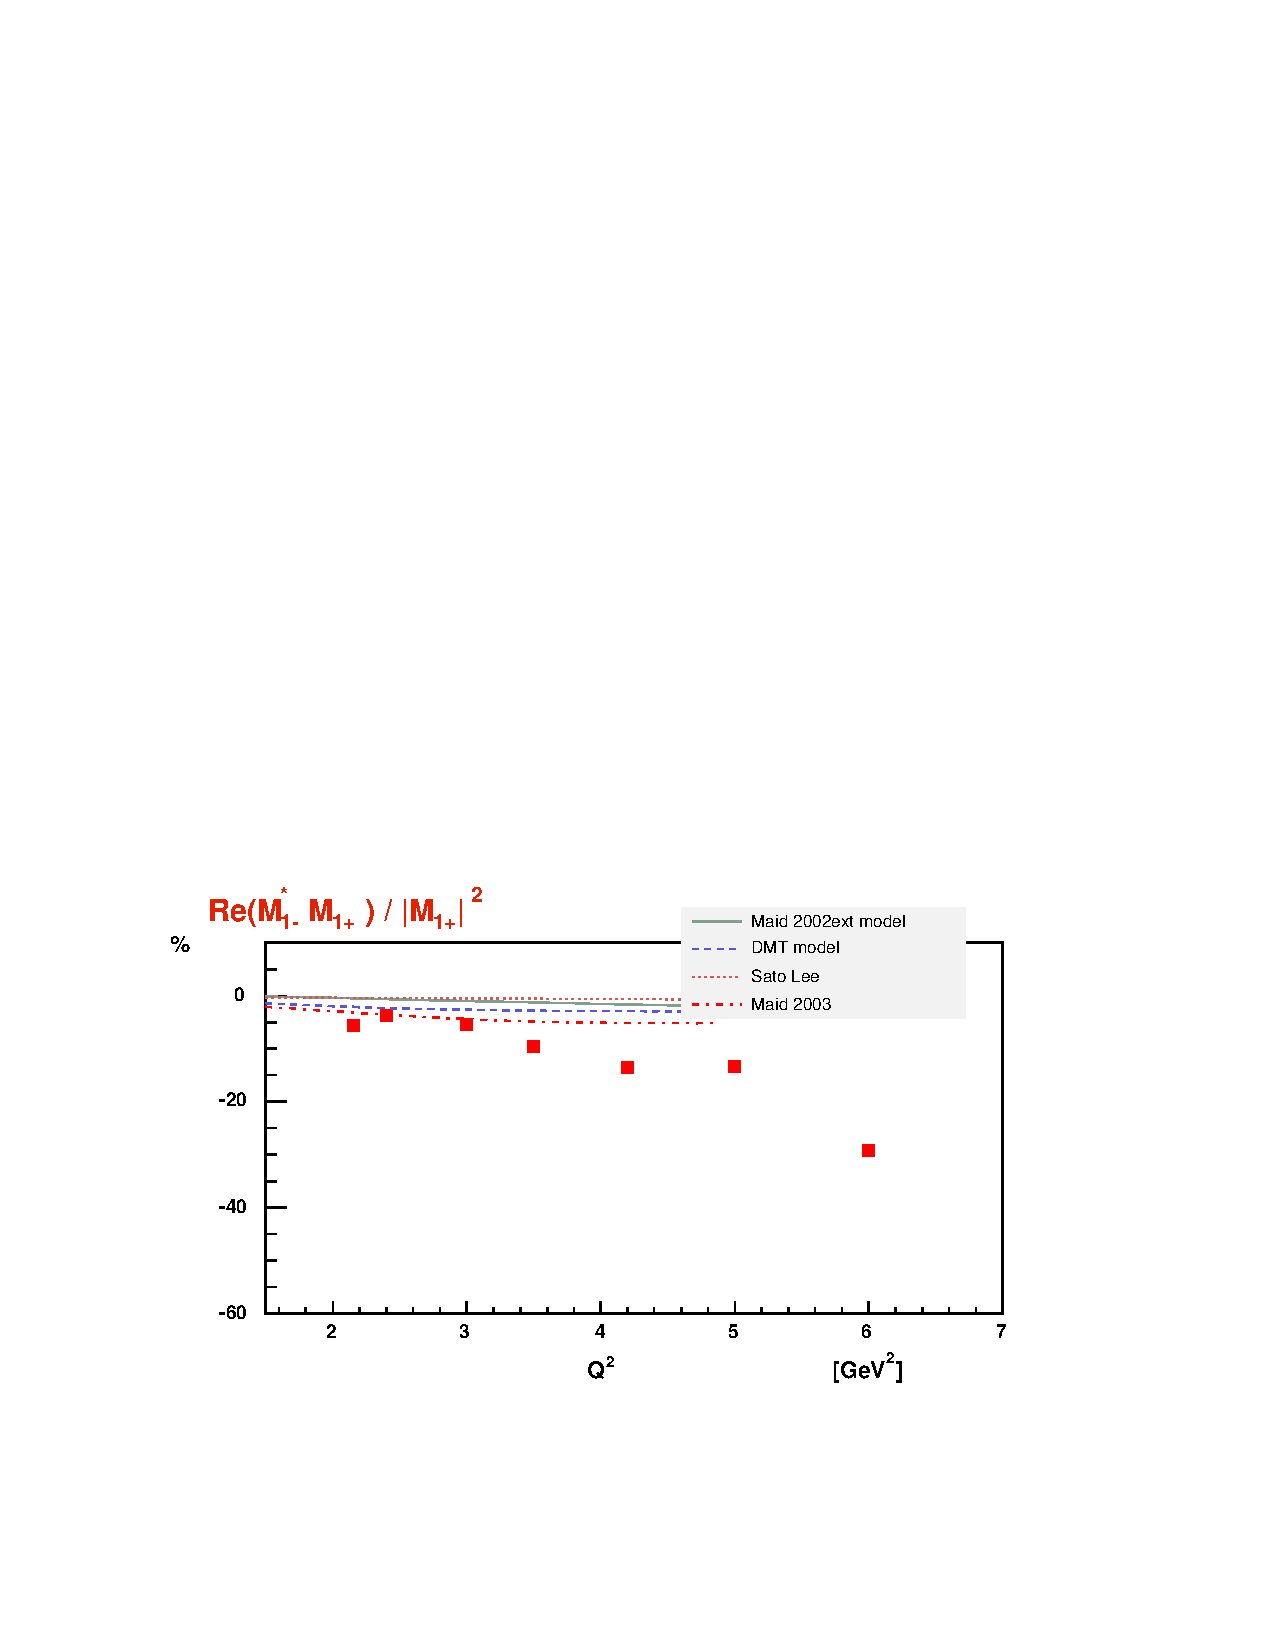
\includegraphics[width = 11cm, bb=30 120 520 400]{analysis/img/M1m} 
  \caption[Amplitude of $M_{1-}$]
{  Result for  $M_{1-}$ as a function of $Q^2$ obtained in the $M_{1+}$ dominance approximation.}
 \label{fig:M1m}

\end{center}
\end{figure}
\begin{figure}[h]
 \begin{center}
 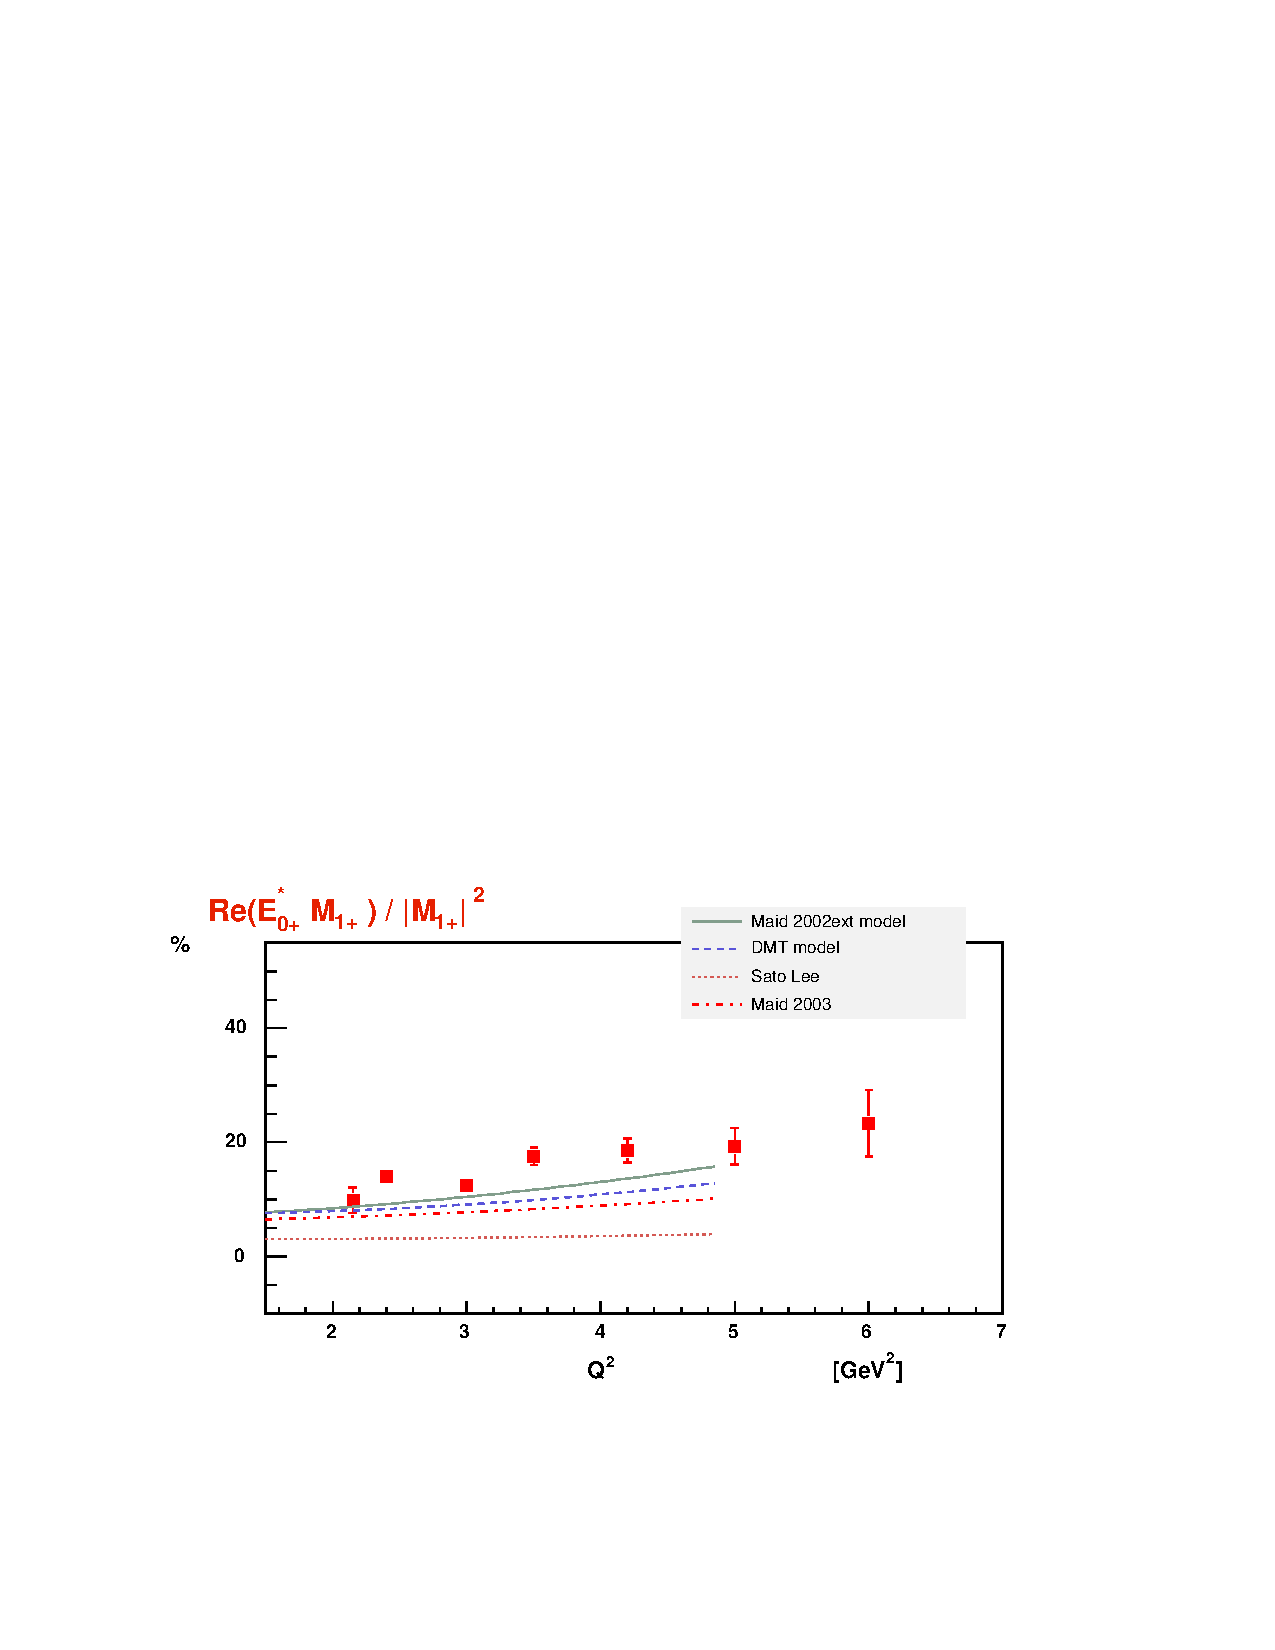
\includegraphics[width = 11cm, bb=30 120 520 400]{analysis/img/E0p} 
 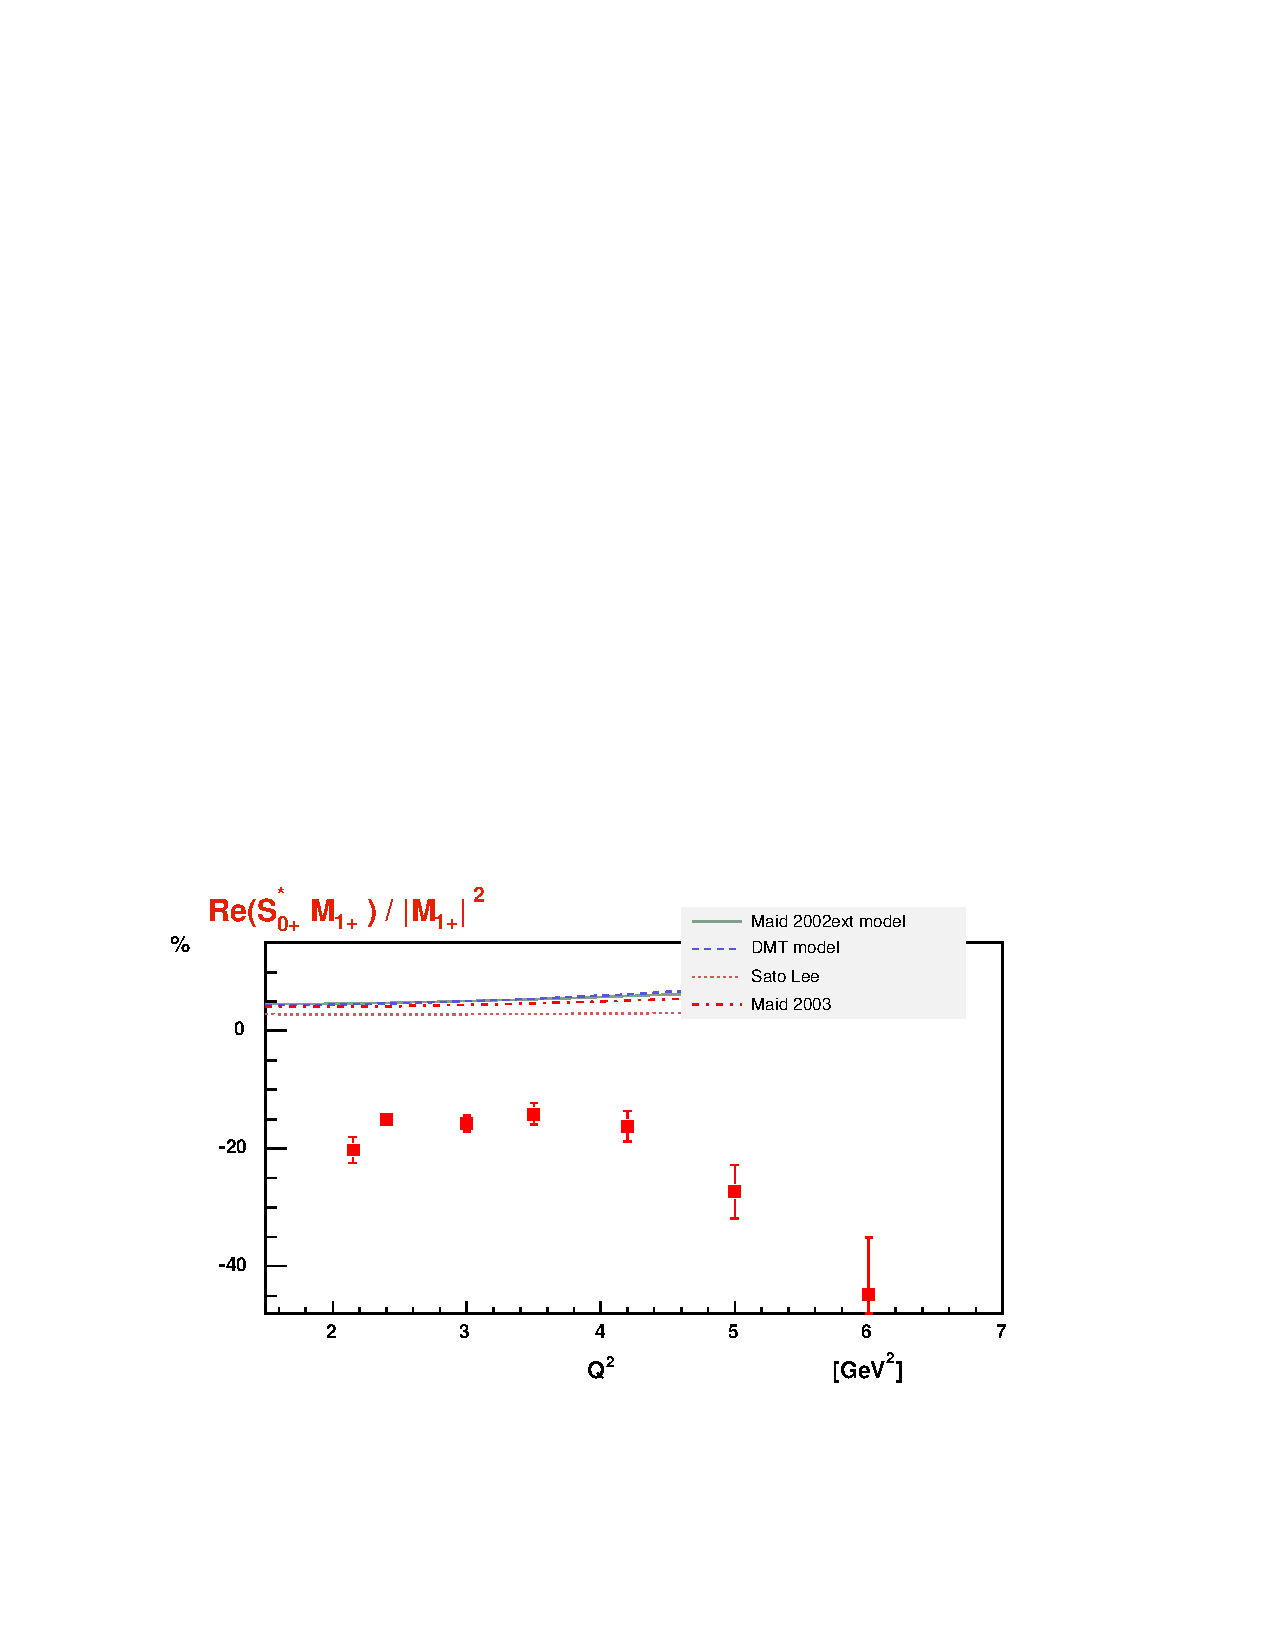
\includegraphics[width = 11cm, bb=30 110 520 400]{analysis/img/S0p} 
  \caption[Amplitudes of $E_{0+}$ and $S_{0+}$]
{  Result for  $E_{0+}$ and $S_{0+}$ as a function of $Q^2$ obtained in the $M_{1+}$ dominance approximation.}
 \label{fig:E0p}
\end{center}
\end{figure}

















\cia  \vspace{-2cm}
\section{The JANR fit}
The JANR model \cite{bib:Inna1}, \cite{bib:Inna2} incorporates the unitary isobar approach \cite{bib:maid2000}
modified in order to
include the Regge poles. The resonances contribute as Breit-Wigner, while non resonant background is built 
from the
Born terms and the {\it t}-channel $\rho$ and $\omega$ contributions. To calculate the Born terms
the latest calculation of
the nucleon and pion form factors was used. 

The parameters obtained by fitting the cross section data are the magnitudes of the multipoles
corresponding to the resonance from the first and second resonance regions at the resonance positions.
After extracting the multipoles, the JANR program can recalculate the cross section. An example of this process is illustrated
in \F{fig:cro_phi_W1.23_Q23.50_Inn} where both the data (blue triangles) and the JANR cross section (solid black line) are plotted.
The JANR global fit well reproduces the experimental data behaviour. 

\begin{figure}[h]
 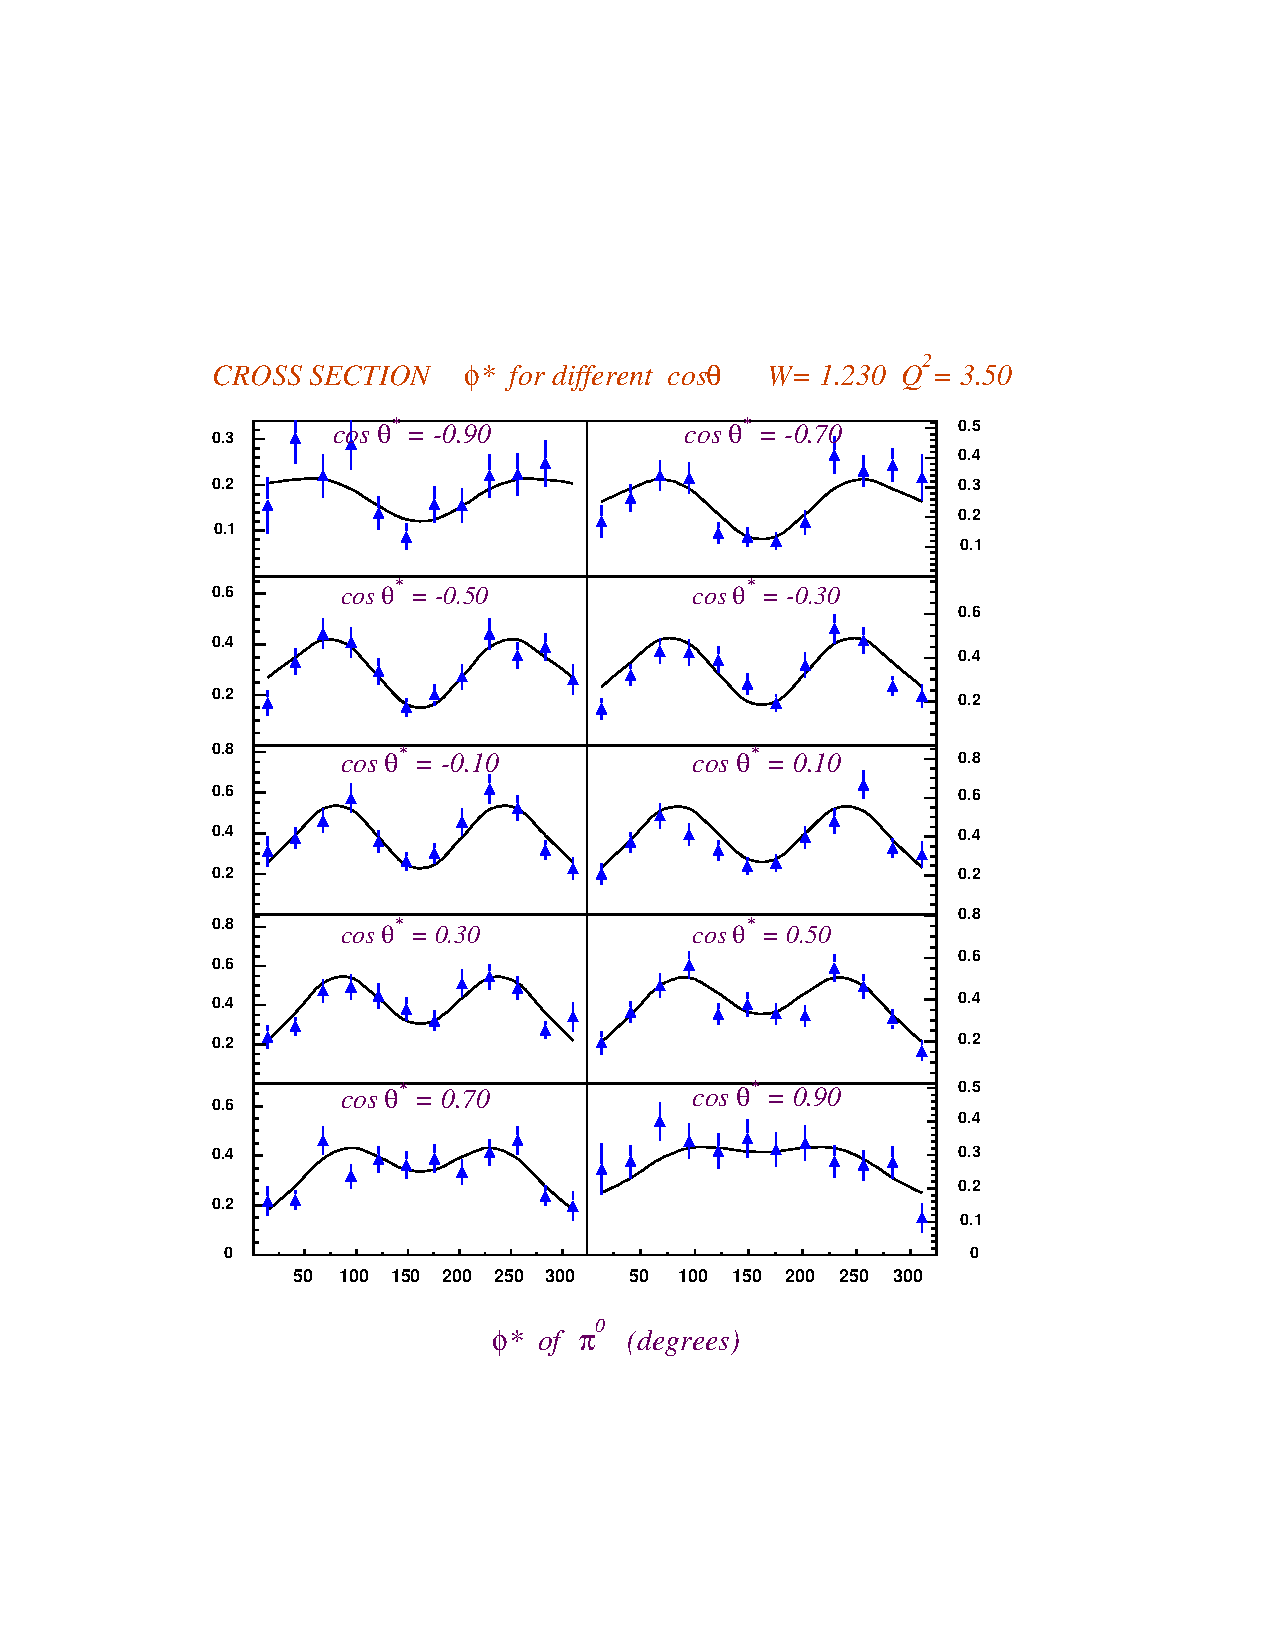
\includegraphics[width = 13cm, bb=-30 140 520 640]{analysis/img/cro_phi_W1.23_Q23.50_Inn}
  \caption[JANR fit of the cross section.]
{ JANR fit of the cross section. The blue triangles represent the experimental data points. The solid black line
 is the JANR calculated cross section after the fit.}
 \label{fig:cro_phi_W1.23_Q23.50_Inn}
\end{figure}

\cia
To further investigate the JANR fit result, the JANR obtained cross section was fitted with Legendre polynomials
as described in \ref{sec:structure}, 
and the structure functions were extracted. An example is shown in \F{fig:lpt_Q23.50_Inn_L1}, 
\F{fig:lt_Q23.50_Inn_L1} and \F{fig:tt_Q23.50_Inn_L1}, where $\sigma_T+\epsilon_L\sigma_L$, $\sigma_{LT}$ and $\sigma_{TT}$ 
are shown respectively.

\begin{figure}[h]
 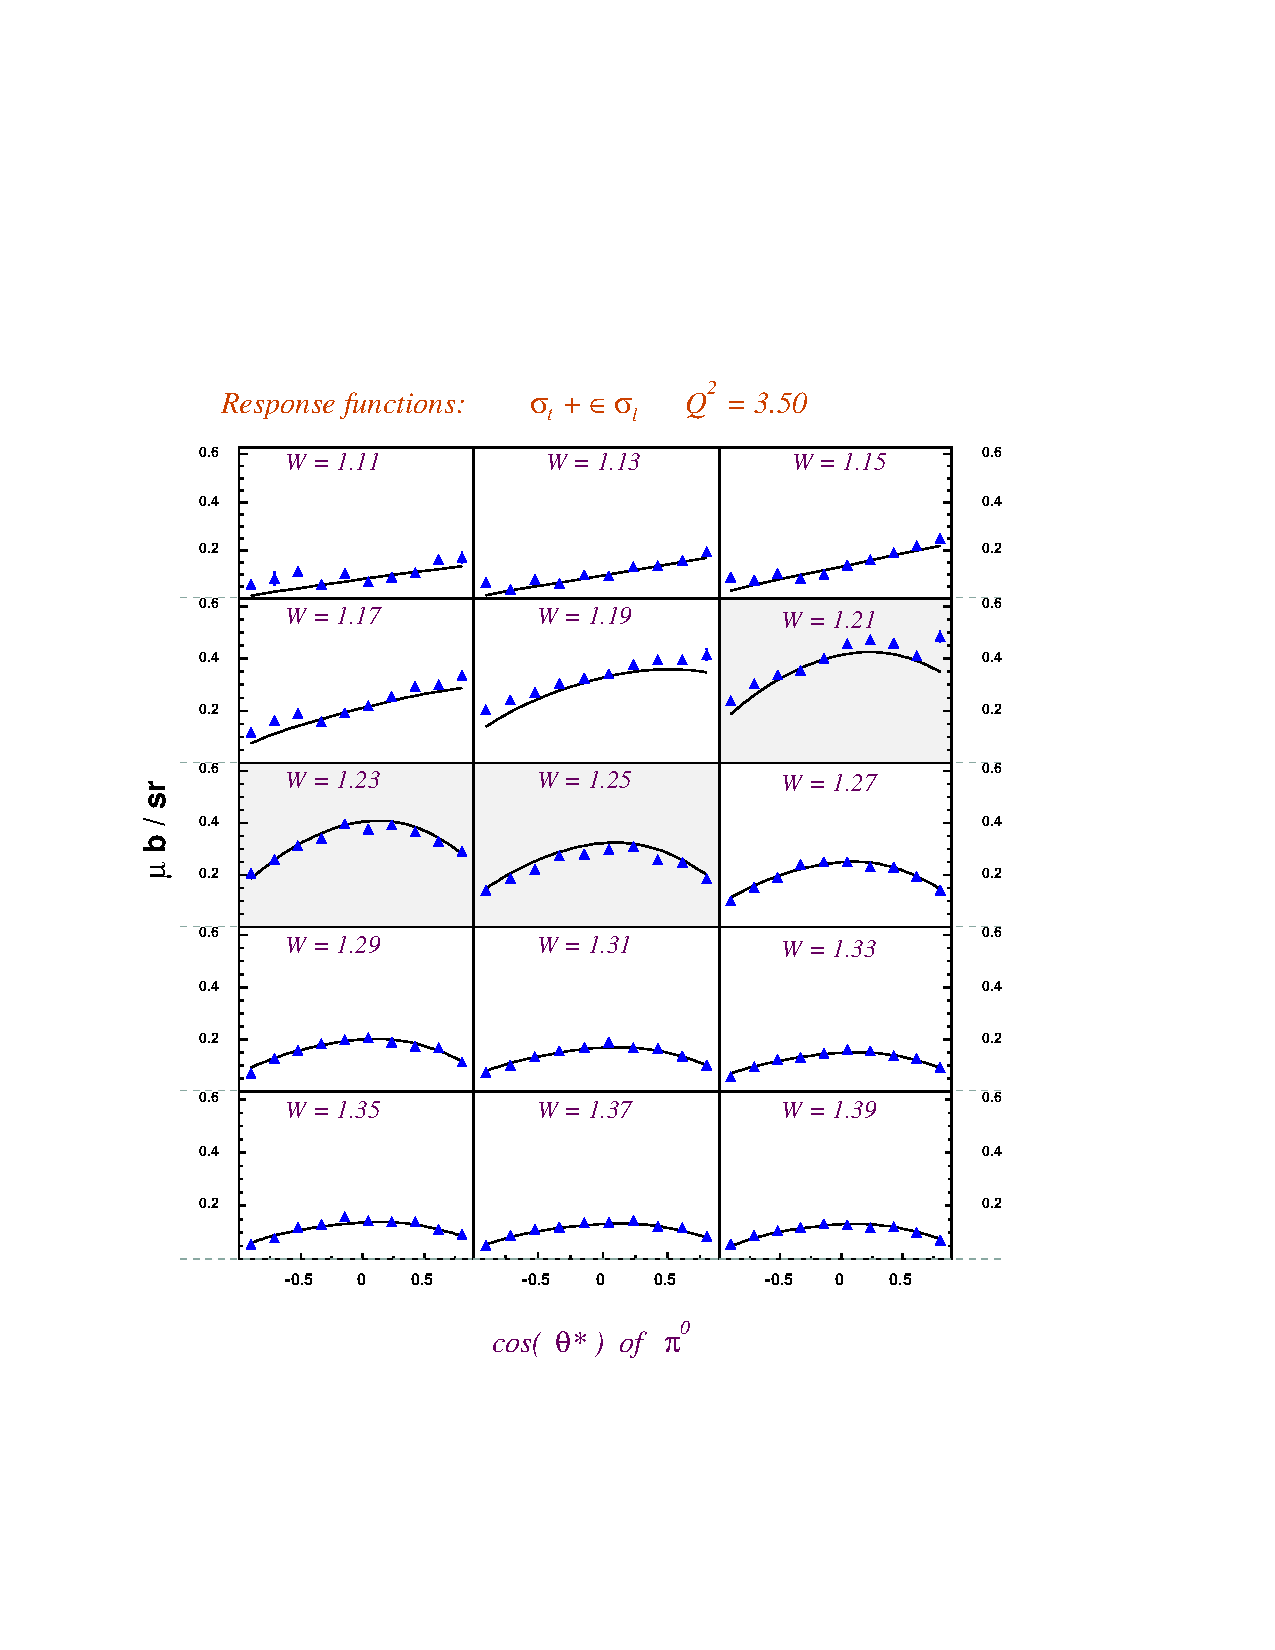
\includegraphics[width = 13cm, bb=-30 140 480 640]{analysis/img/lpt_Q23.50_Inn_L1}
  \caption[JANR fit of the cross section: $\sigma_T+\epsilon_L\sigma_L$]
{ JANR fit and  $\sigma_T+\epsilon_L\sigma_L$. The blue triangles represent the experimental data points. The solid black line
 is the JANR calculated cross section after the JANR fit.}
 \label{fig:lpt_Q23.50_Inn_L1}
\end{figure}

\begin{figure}[h]
 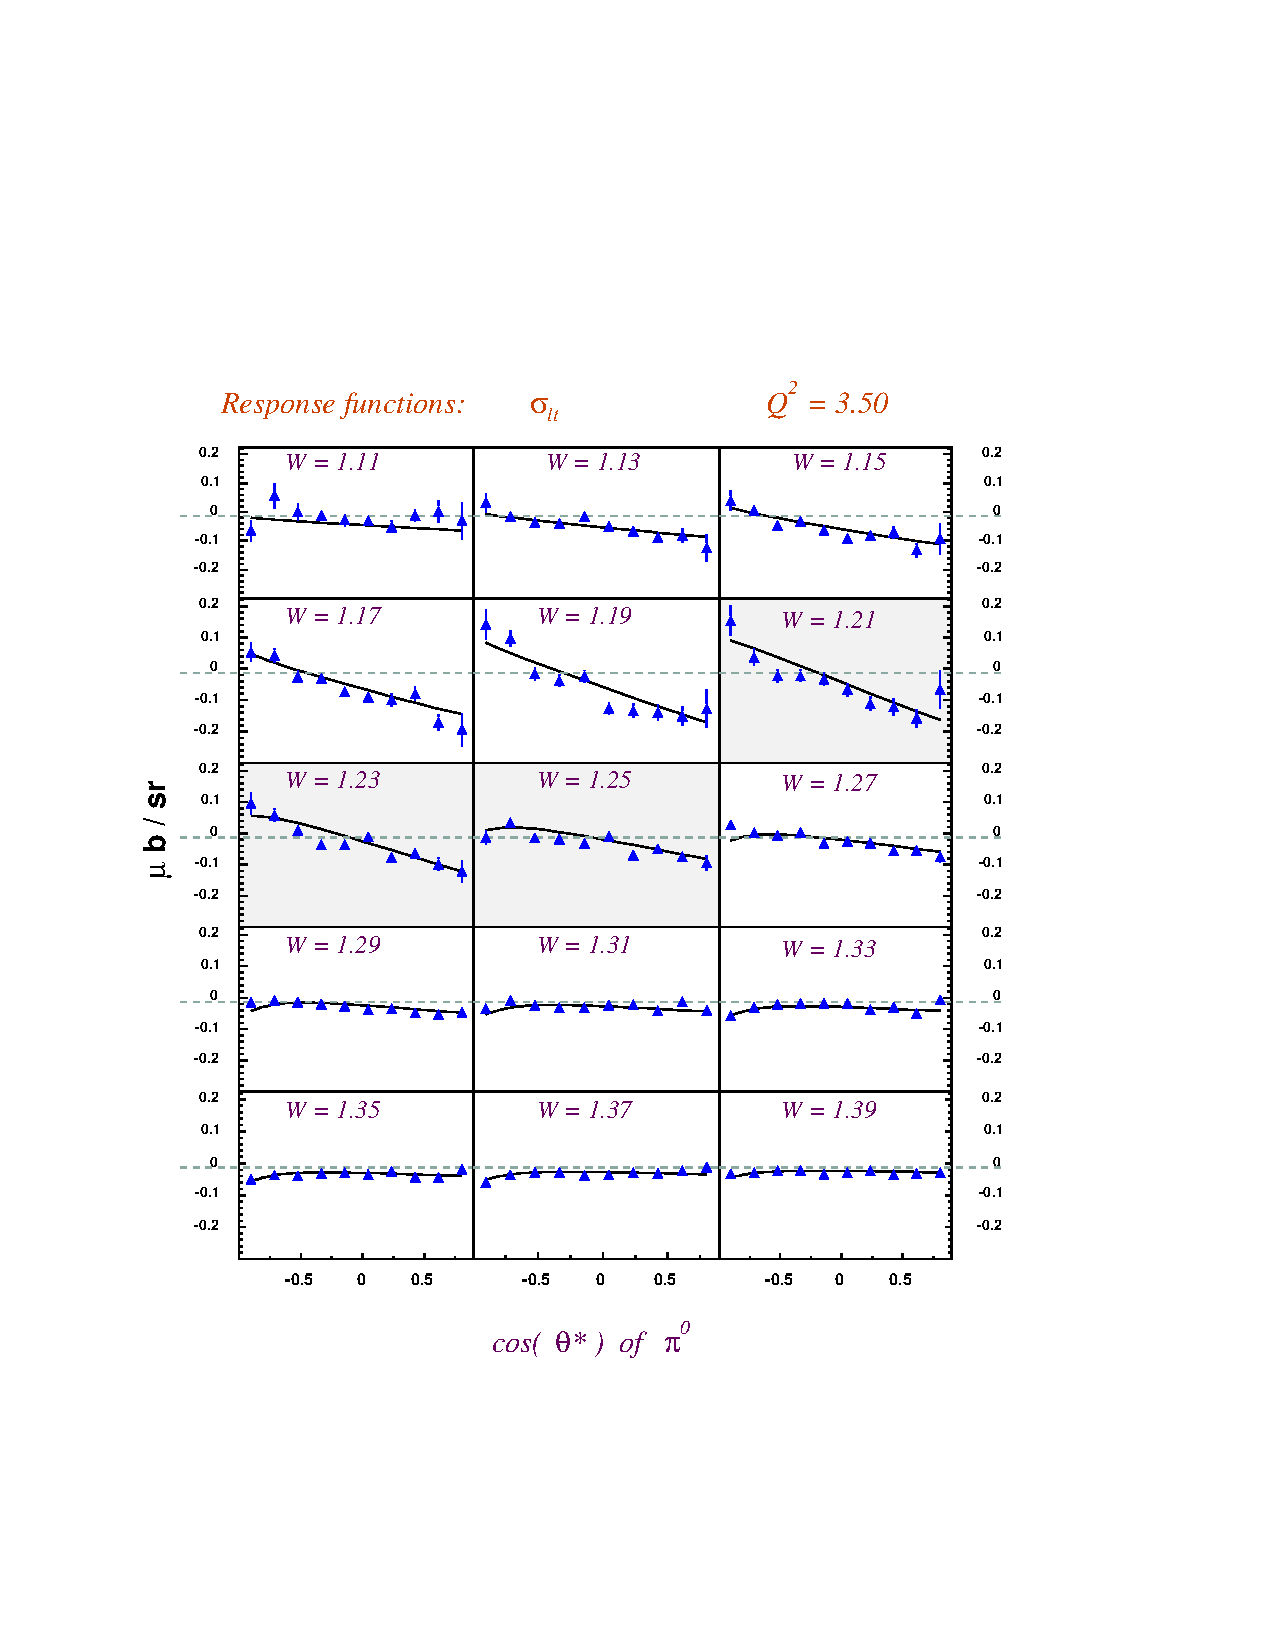
\includegraphics[width = 13cm, bb=-30 140 480 640]{analysis/img/slt_Q23.50_Inn_L1}
  \caption[JANR fit of the cross section: $\sigma_T+\epsilon_L\sigma_L$]
{ JANR fit and  $\sigma_{LT}$. The blue triangles represent the experimental data points. The solid black line
 is the JANR calculated cross section after the JANR fit.}
 \label{fig:lt_Q23.50_Inn_L1}
\end{figure}

\begin{figure}[h]
 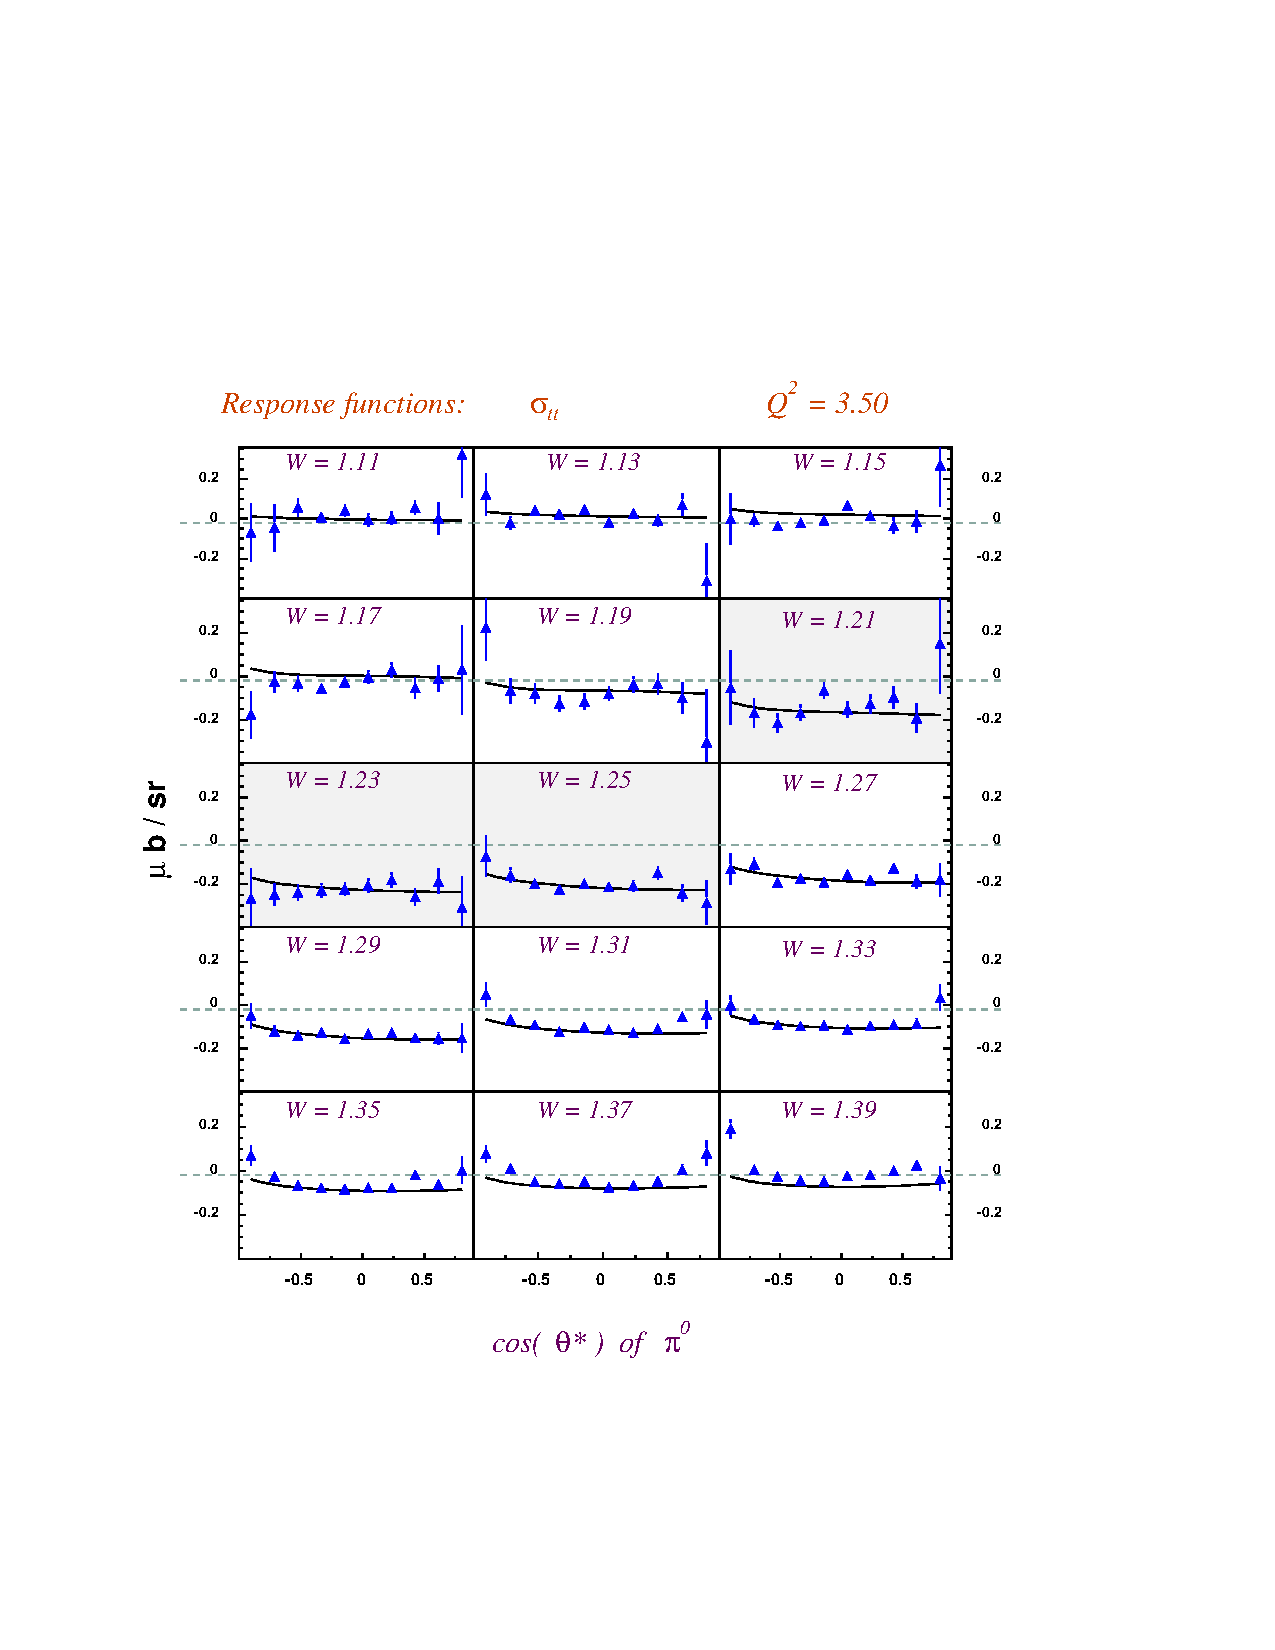
\includegraphics[width = 13cm, bb=-30 140 480 640]{analysis/img/stt_Q23.50_Inn_L1}
  \caption[JANR fit of the cross section: $\sigma_T+\epsilon_L\sigma_L$]
{ JANR fit and  $\sigma_{TT}$. The blue triangles represent the experimental data points. The solid black line
 is the JANR calculated cross section after the JANR fit.}
 \label{fig:tt_Q23.50_Inn_L1}
\end{figure}

\cia  \vspace{-2cm}
\subsection{JANR Results for $R_{EM}$ and $R_{SM}$}
In \F{fig:JANRREM} and \F{fig:JANRRSM} the results for $R_{EM}$ and $R_{SM}$ of the JANR fit is shown.
While $R_{SM}$ is consistent with the multipole truncation result, $R_{EM}$  presents  significantly lower values.
To investigate this discrepancy, the JANR obtained cross section was analyzed using the multipole truncation method.
The result for $R_{EM}$ is shown in \F{fig:JANRREMtrunc}, where one can see that the multipole truncation
introduce a systematic shift on $R_{EM}$, increasing in value with $Q^2$.
The result in \F{fig:JANRREMtrunc} is somewhat consistent with the multipole truncated analysis fit of the experimental 
data shown in \F{fig:RM}.

When comparing the JANR fit of this data with the previous Hall-C data, a significantly smaller value for the 
$M_{1-}$ amplitude is found. See Sec. \ref{sec:other_models}

\begin{figure}[h]
 \begin{center}
 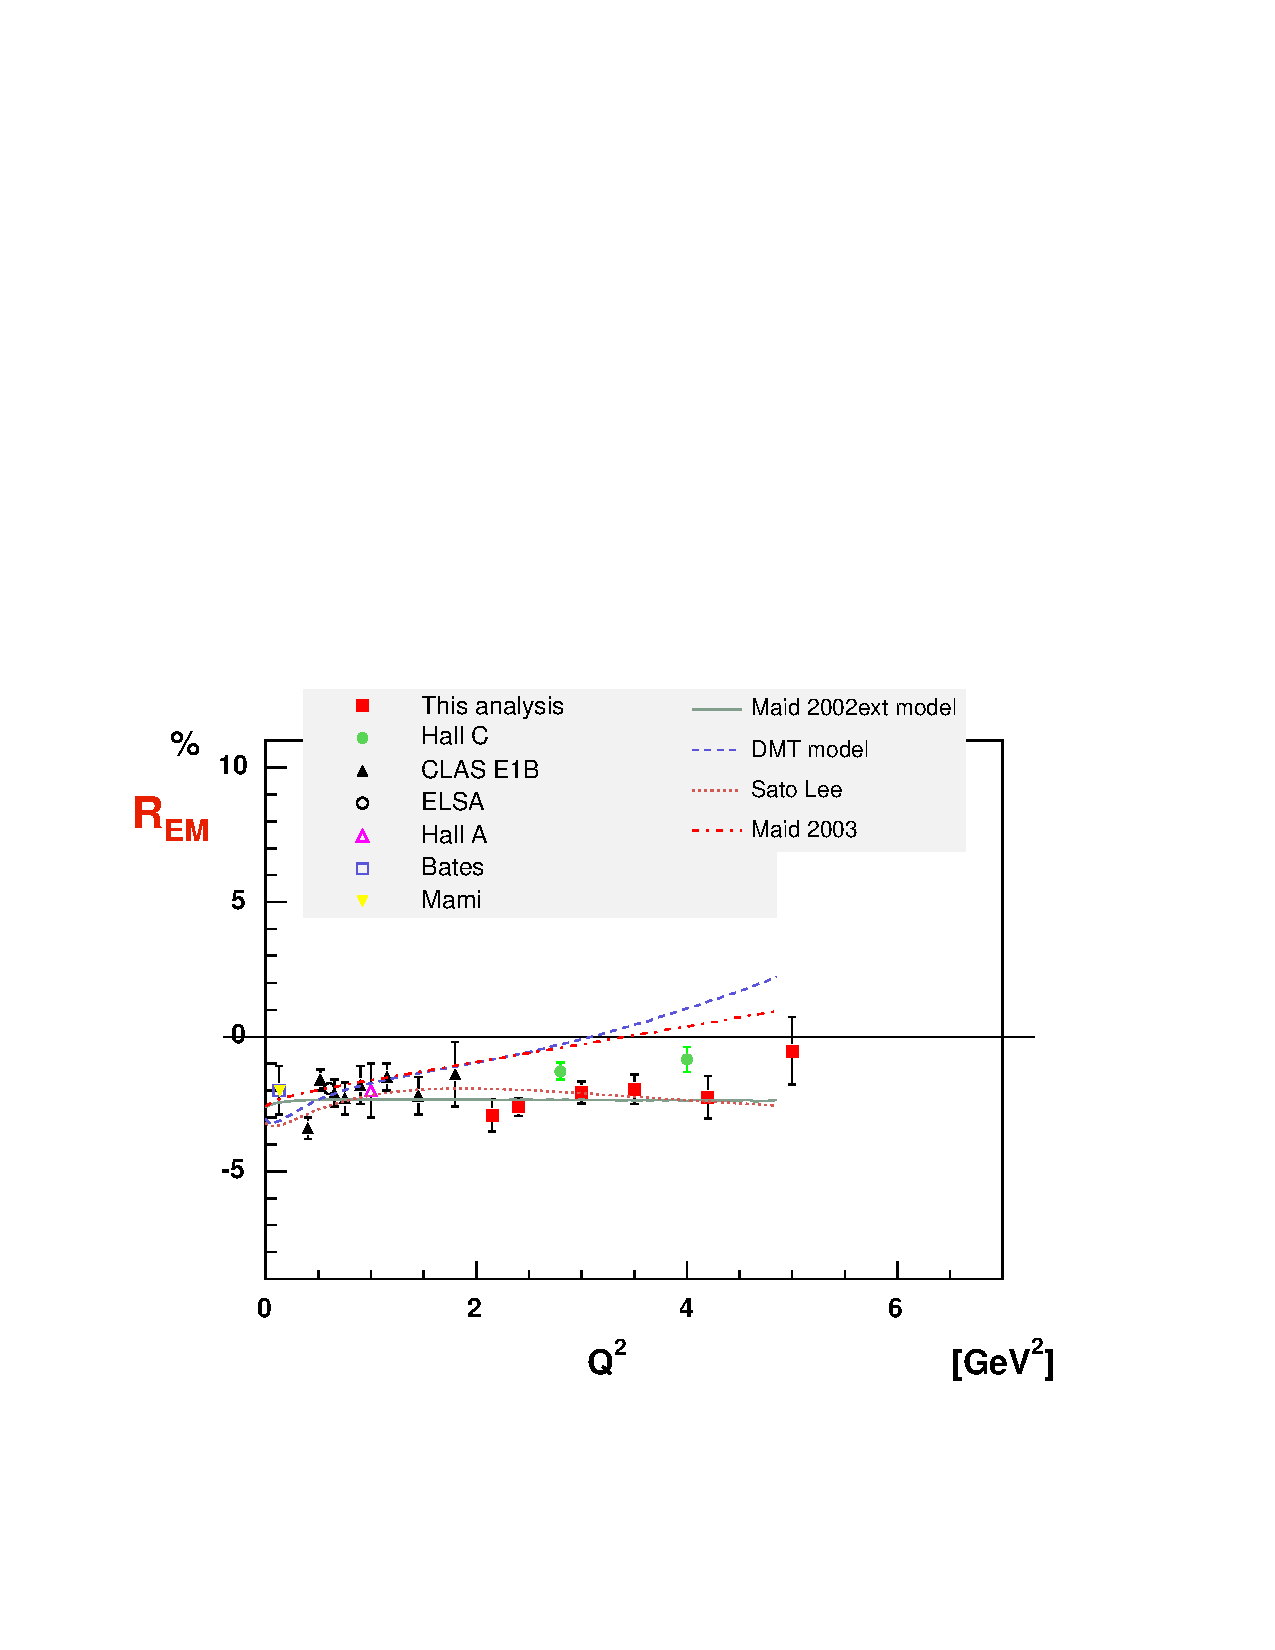
\includegraphics[width = 13cm, bb=30 130 540 500]{analysis/img/JANR_REM} 
  \caption[JANR result for $R_{EM}$ as a function of $Q^2$]
{  Result for $R_{EM}$ as a function of $Q^2$ obtained with JANR.}
 \label{fig:JANRREM}
\end{center}
\end{figure}


\begin{figure}[h]
 \begin{center}
 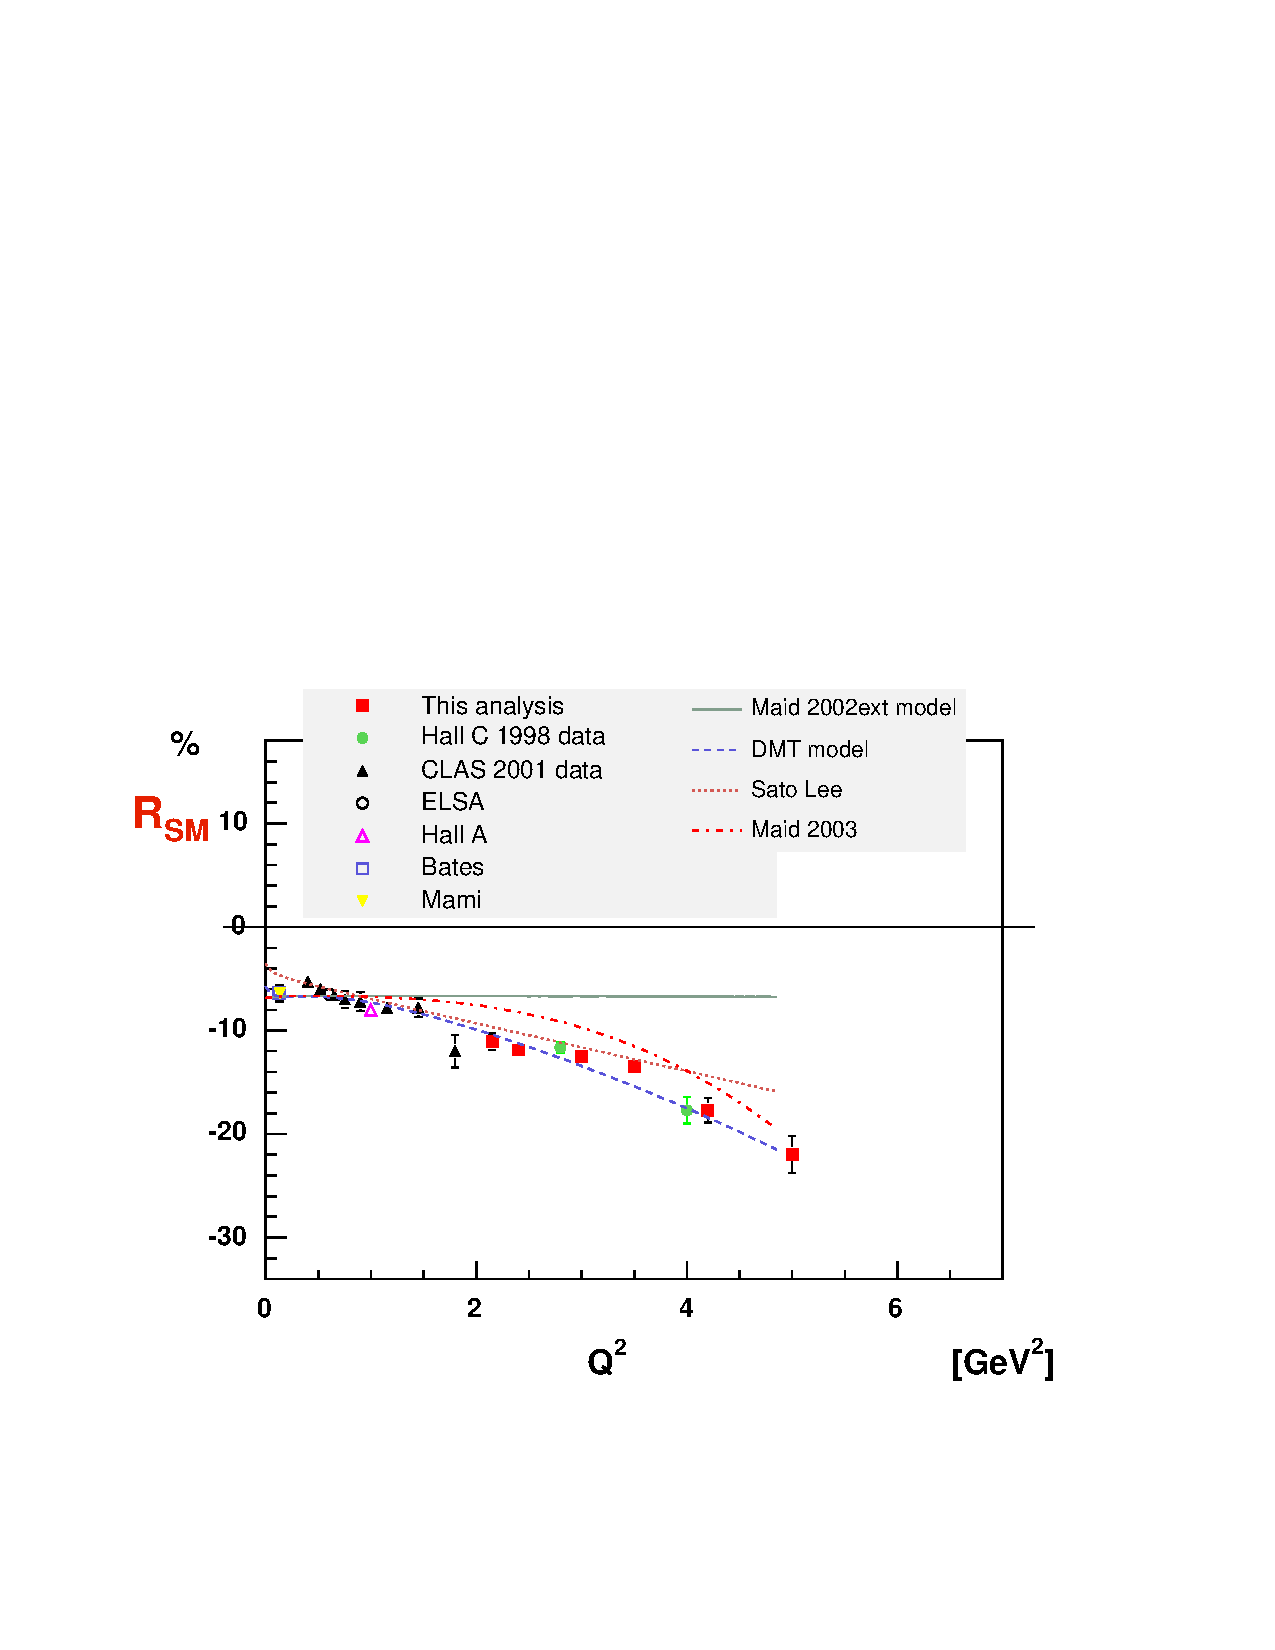
\includegraphics[width = 13cm, bb=30 130 540 500]{analysis/img/JANR_RSM} 
  \caption[JANR result for $R_{SM}$ as a function of $Q^2$]
{  Result for $R_{SM}$ as a function of $Q^2$ obtained with JANR.}
 \label{fig:JANRRSM}
\end{center}
\end{figure}

\begin{figure}[h]
 \begin{center}
 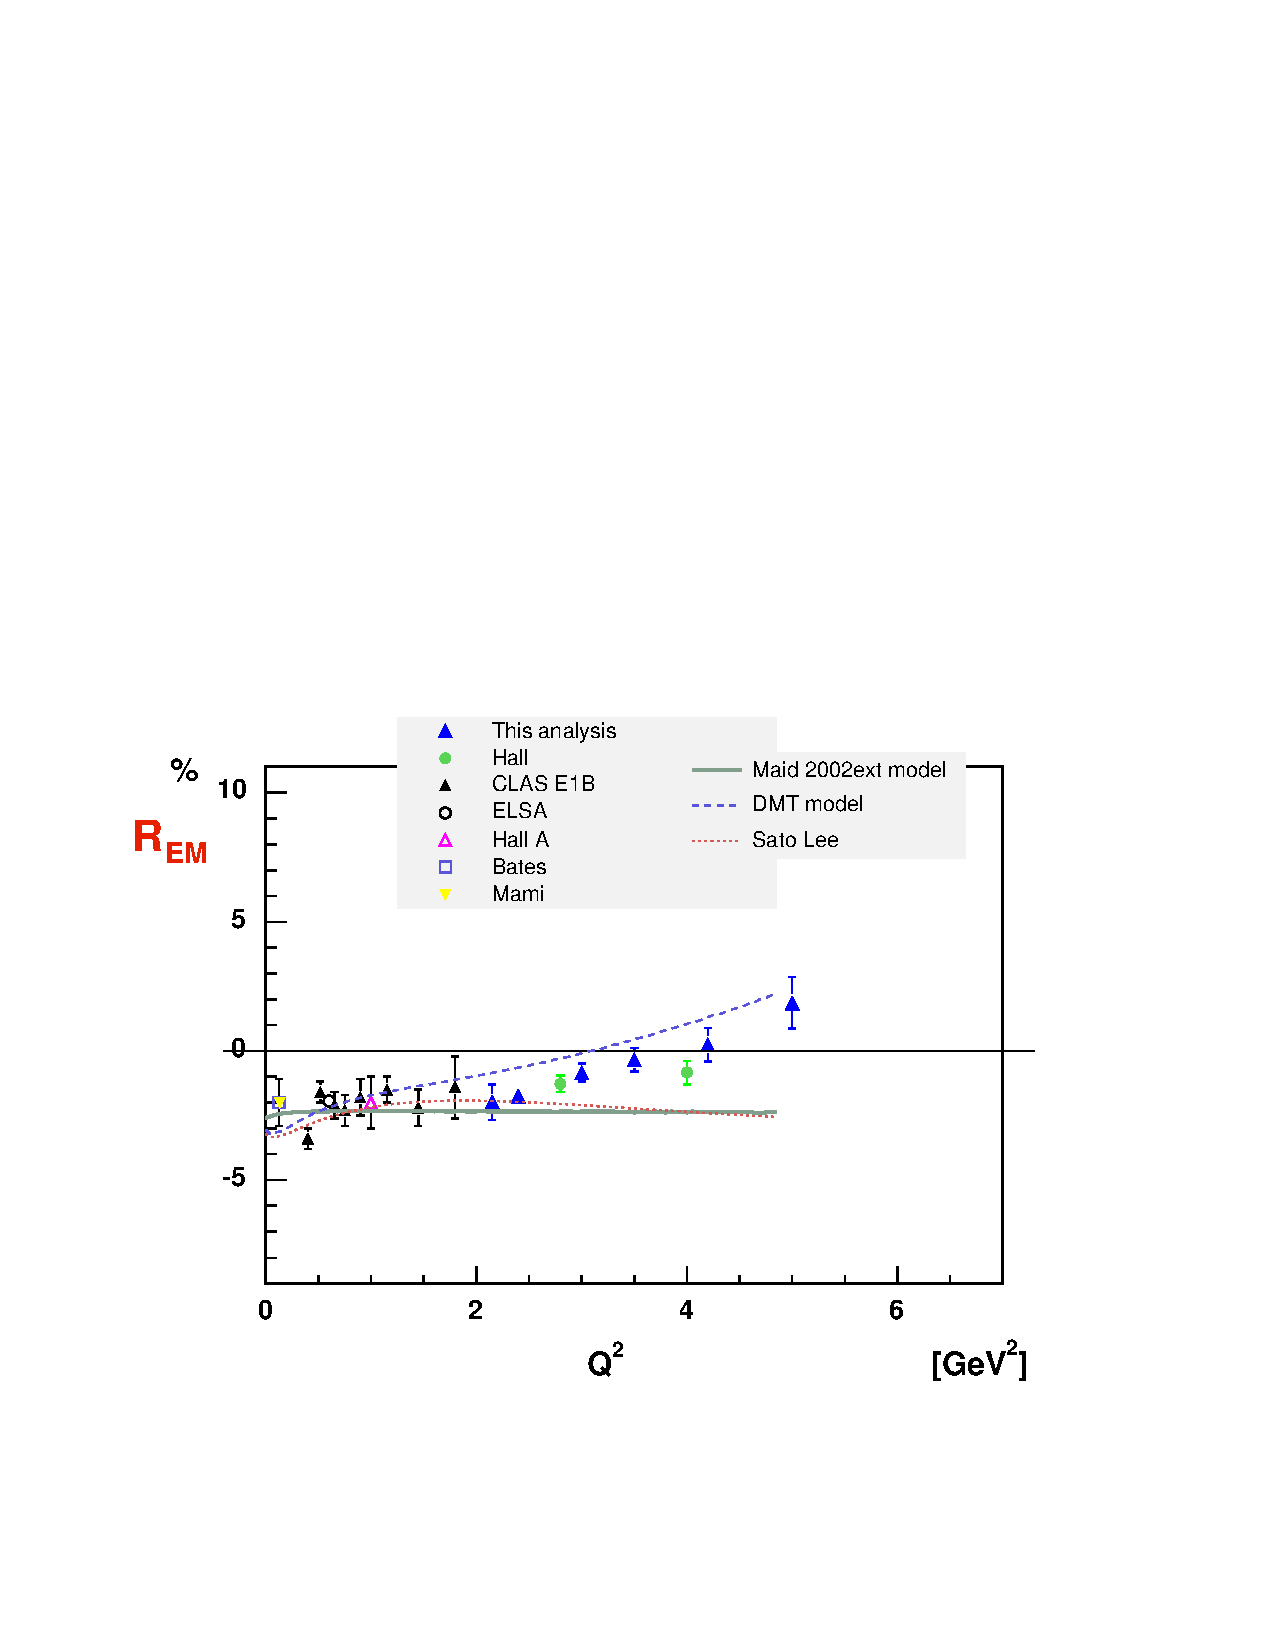
\includegraphics[width = 13cm, bb=30 130 540 500]{analysis/img/JANR_truncated} 
  \caption[JANR truncated result for $R_{EM}$ as a function of $Q^2$]
{  Result for $R_{EM}$ as a function of $Q^2$ obtained applying the multipole truncation method
  to the JANR obtained cross section. Compare this plot with \F{fig:JANRREM} to see how much the 
  result changes with the fit method used. Compare this plot with \F{fig:RM} to see the multipole
  truncation fit to the real data.}
 \label{fig:JANRREMtrunc}
\end{center}
\end{figure}
 

\cia
\section{Different models and the $P_{11}$ signal}\label{sec:other_models}
The data has been compared with the models {\sl maid2000 }, {\sl maid2002ext}, 
{\sl maid2003} \cite{bib:maid2000}\footnote{see also {\tt http://www.kph.uni-mainz.de/MAID } }
{\sl DMT2001} \cite{bib:dmt2001}. When using the maid2003 model, the cross section
has been calculated with or without the $P_{11}$ resonance.
The data has also been compared with the cross section calculated by JANR as a result of the fit
to this data as a check for consistency.
All the cross sections, response functions, coefficient, multipoles distributions can be found
on the web at, respectively:
\begin{verbatim} 
http://www.jlab.org/~ungaro/pi0eprod/cro_plots
http://www.jlab.org/~ungaro/pi0eprod/responses
http://www.jlab.org/~ungaro/pi0eprod/coefficients
http://www.jlab.org/~ungaro/pi0eprod/multipoles
http://www.jlab.org/~ungaro/pi0eprod/results
\end{verbatim}
by clicking the appropriate model check box at the top of the page.

Each model cross section has been fitted as described in Sec. \ref{sec:structure}
and the response functions have been expanded in Legendre polynomial. The coefficents
of the expansion have been compared to the real data.
Here we report the comparison of the $A$ coefficients for the Legendre expansion of
$\sigma_T+\epsilon_L\sigma_L$ at $Q^2=3.5$ $GeV^2$ and $\ell\le 2$.

The JANR fit is a good match to the data, as expected. The coefficient $A_2$ is directly linked
to $R_{EM}$ (see Eq. [\ref{eqno:m1dominance}]). Maid 2002 consistently underestimates $A_2$, 
while DMT matches the data at the $\Delta $ peak, but fails at higher $W$ values.
Good agreement is found for the Maid 2003 model.

When turning on and off the $P_{11}$ resonance in the Maid 2003 model (see \F{fig:A_comp_m03a} and \F{fig:A_comp_m03r})
one can see differences in the $A_0$ and $A_1$ coefficients. Without the Roper resonance Maid 2003 seems to 
better reproduce the data. These behaviour is seen at all $Q^2$. 


\begin{figure}[h]
 \begin{center}
 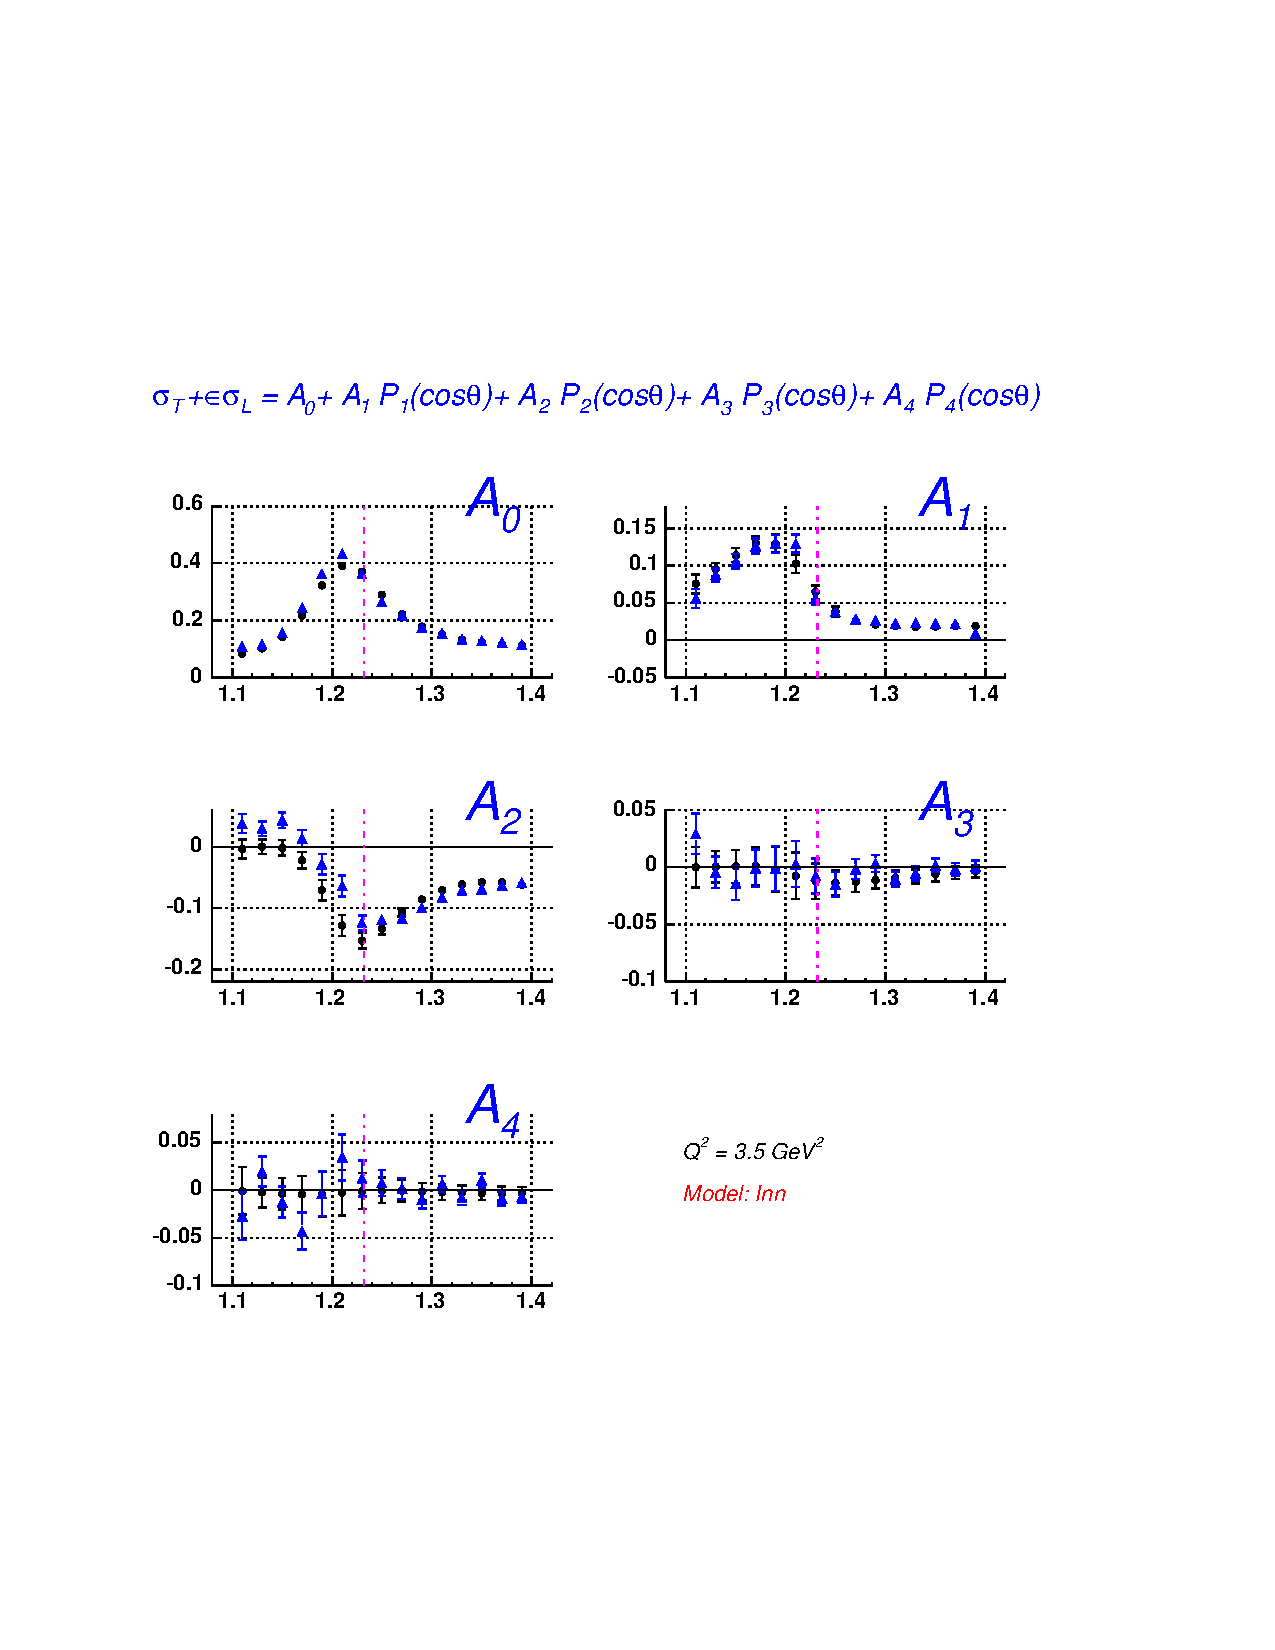
\includegraphics[width = 12cm, bb=30 130 540 700]{analysis/img/A_comp_inna} 
  \caption[Coefficents of the Legendre expansion of $\sigma_T+\epsilon_L\sigma_L$ for the JANR generated cross 
  section  and experimental data ]
{ Coefficents of the Legendre expansion of $\sigma_T+\epsilon_L\sigma_L$ for the JANR generated cross 
  section (black) and experimental data (blue) }
 \label{fig:A_comp_inna}
\end{center}
\end{figure}

\begin{figure}[h]
 \begin{center}
 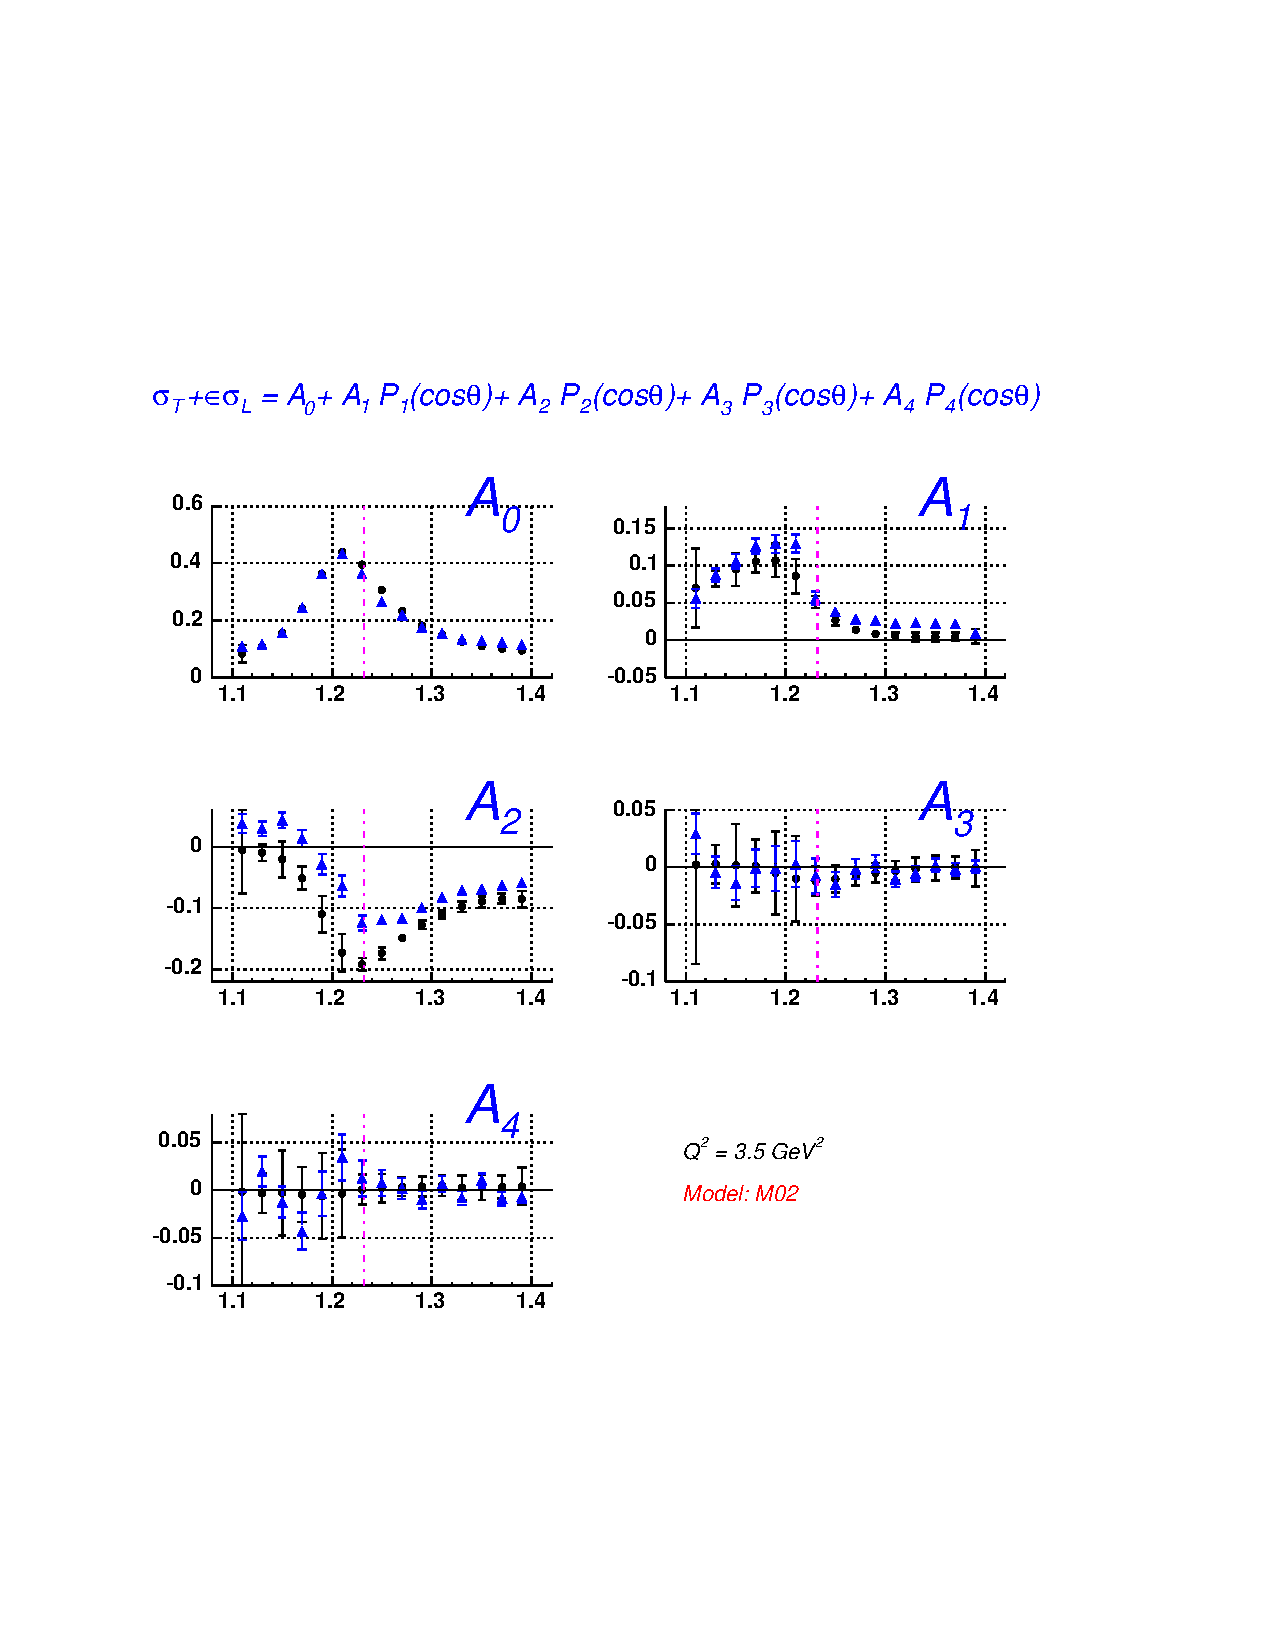
\includegraphics[width = 12cm, bb=30 130 540 700]{analysis/img/A_comp_m02} 
  \caption[Coefficents of the Legendre expansion of $\sigma_T+\epsilon_L\sigma_L$ for the maid 2002 generated cross 
  section  and experimental data ]
{ Coefficents of the Legendre expansion of $\sigma_T+\epsilon_L\sigma_L$ for the maid 2002 generated cross 
  section (black) and experimental data (blue) }
 \label{fig:A_comp_m02}
\end{center}
\end{figure}

\begin{figure}[h]
 \begin{center}
 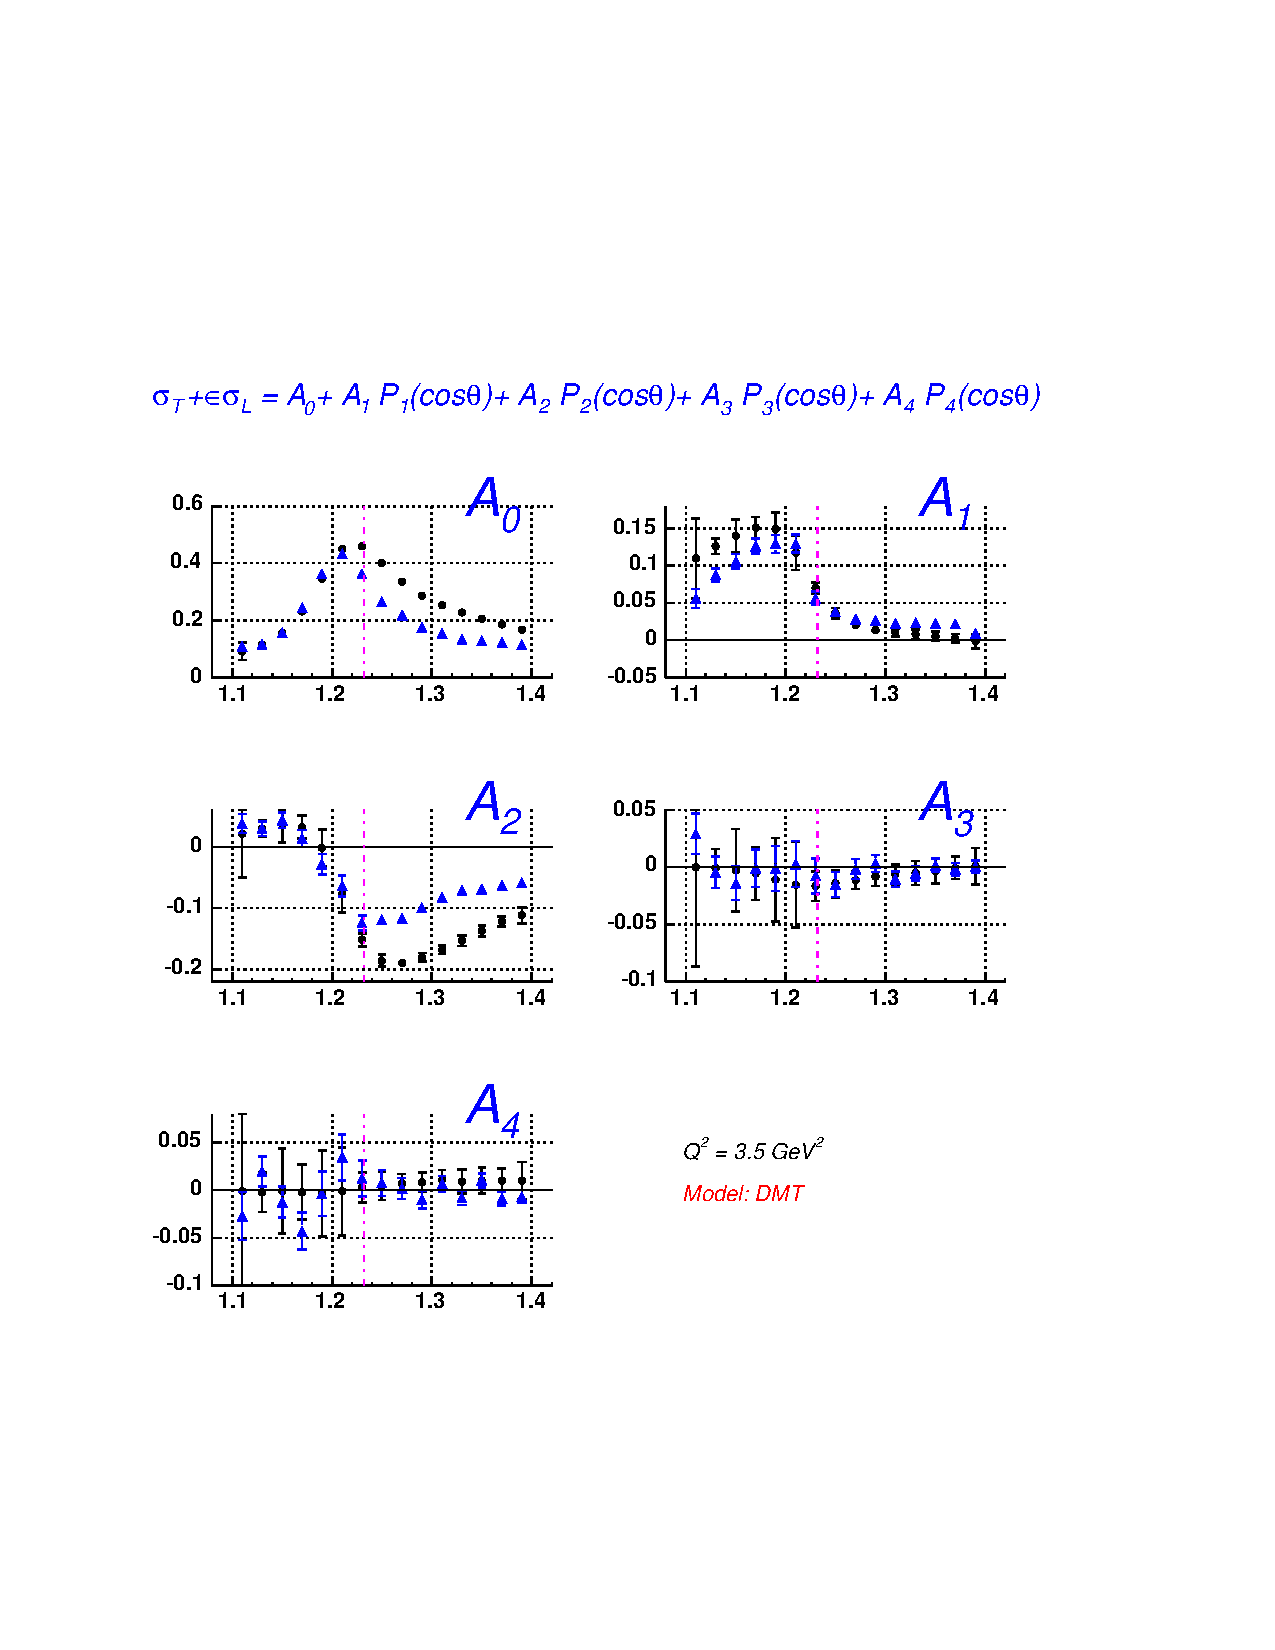
\includegraphics[width = 12cm, bb=30 130 540 700]{analysis/img/A_comp_dmt} 
  \caption[Coefficents of the Legendre expansion of $\sigma_T+\epsilon_L\sigma_L$ for the DMT generated cross 
  section  and experimental data ]
{ Coefficents of the Legendre expansion of $\sigma_T+\epsilon_L\sigma_L$ for the DMT generated cross 
  section (black) and experimental data (blue) }
 \label{fig:A_comp_dmt}
\end{center}
\end{figure}


\begin{figure}[h]
 \begin{center}
 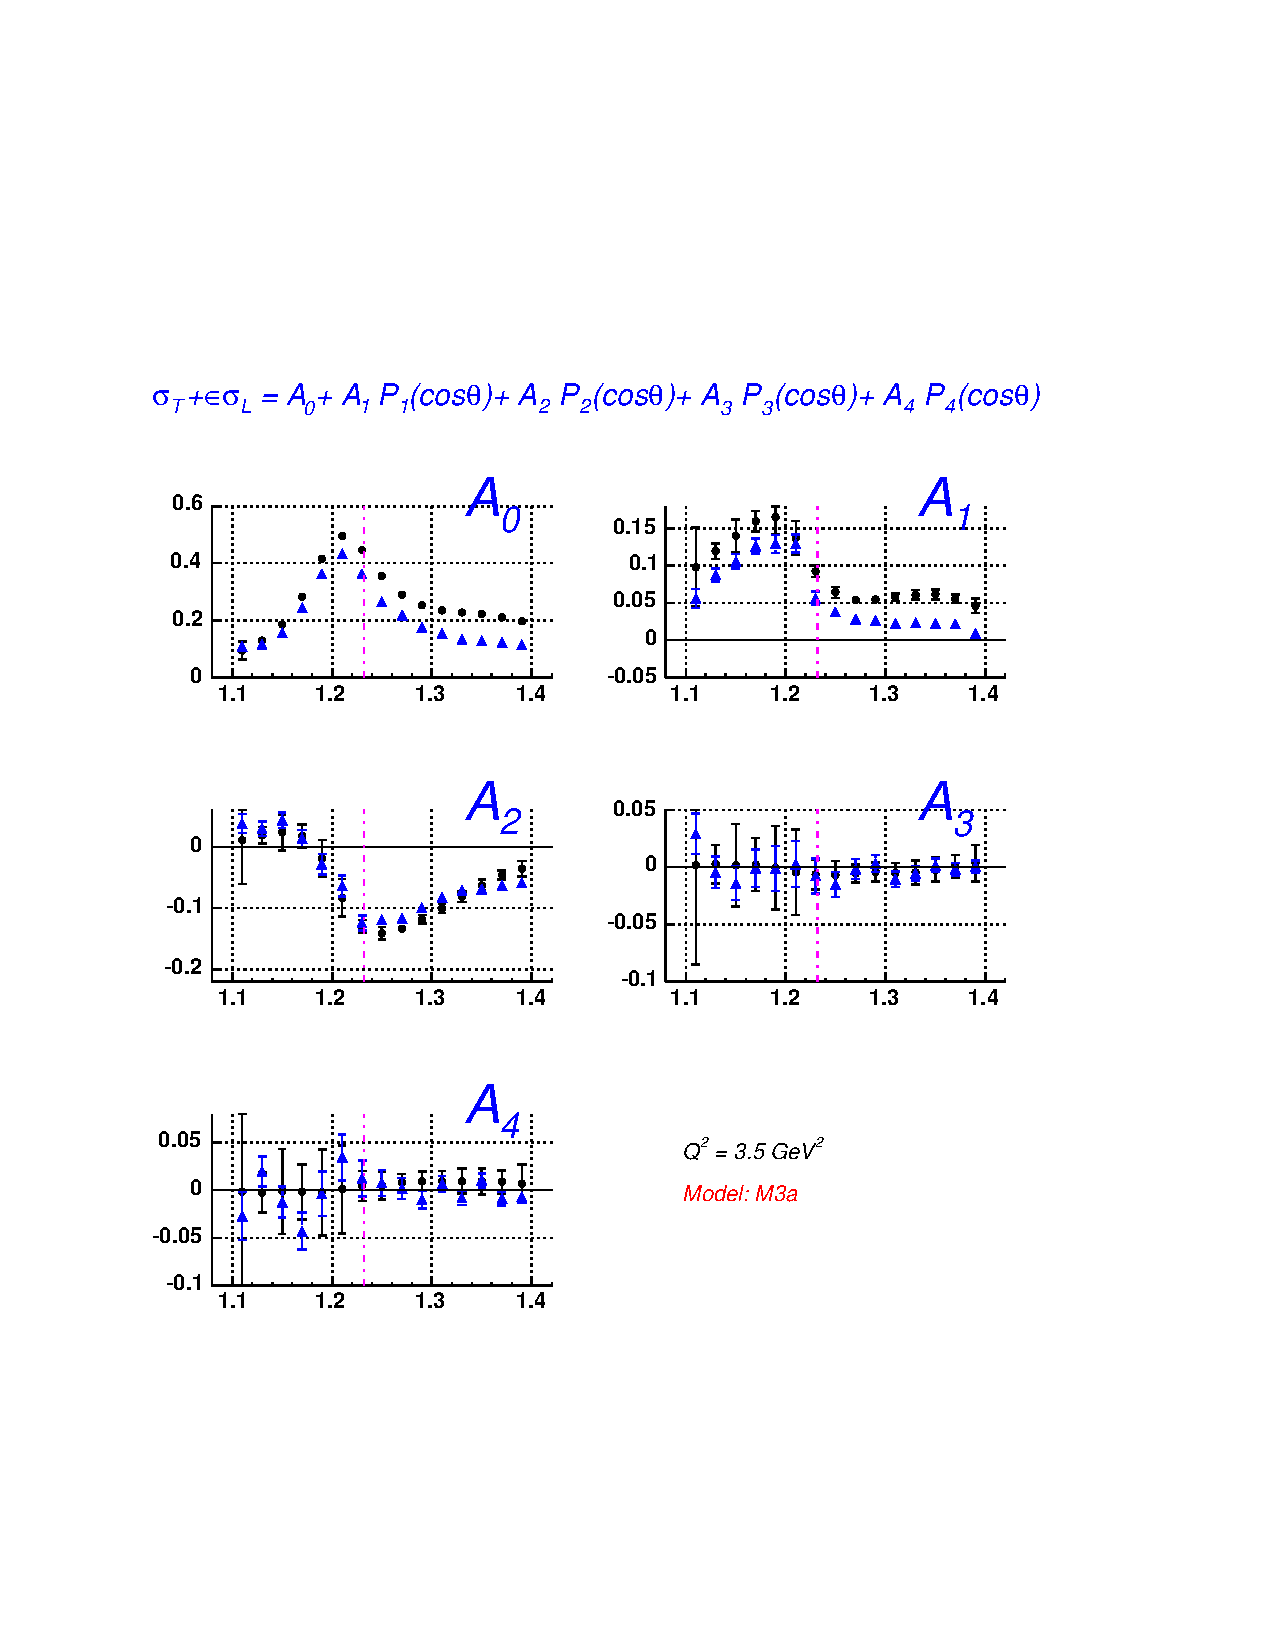
\includegraphics[width = 12cm, bb=30 130 540 700]{analysis/img/A_comp_m03a} 
  \caption[Coefficents of the Legendre expansion of $\sigma_T+\epsilon_L\sigma_L$ for the maid 2003 with Roper {\bf on} 
  generated cross 
  section  and experimental data ]
{ Coefficents of the Legendre expansion of $\sigma_T+\epsilon_L\sigma_L$ for the maid 2003 with Roper {\bf on}  generated cross 
  section (black) and experimental data (blue) }
 \label{fig:A_comp_m03a}
\end{center}
\end{figure}

\begin{figure}[h]
 \begin{center}
 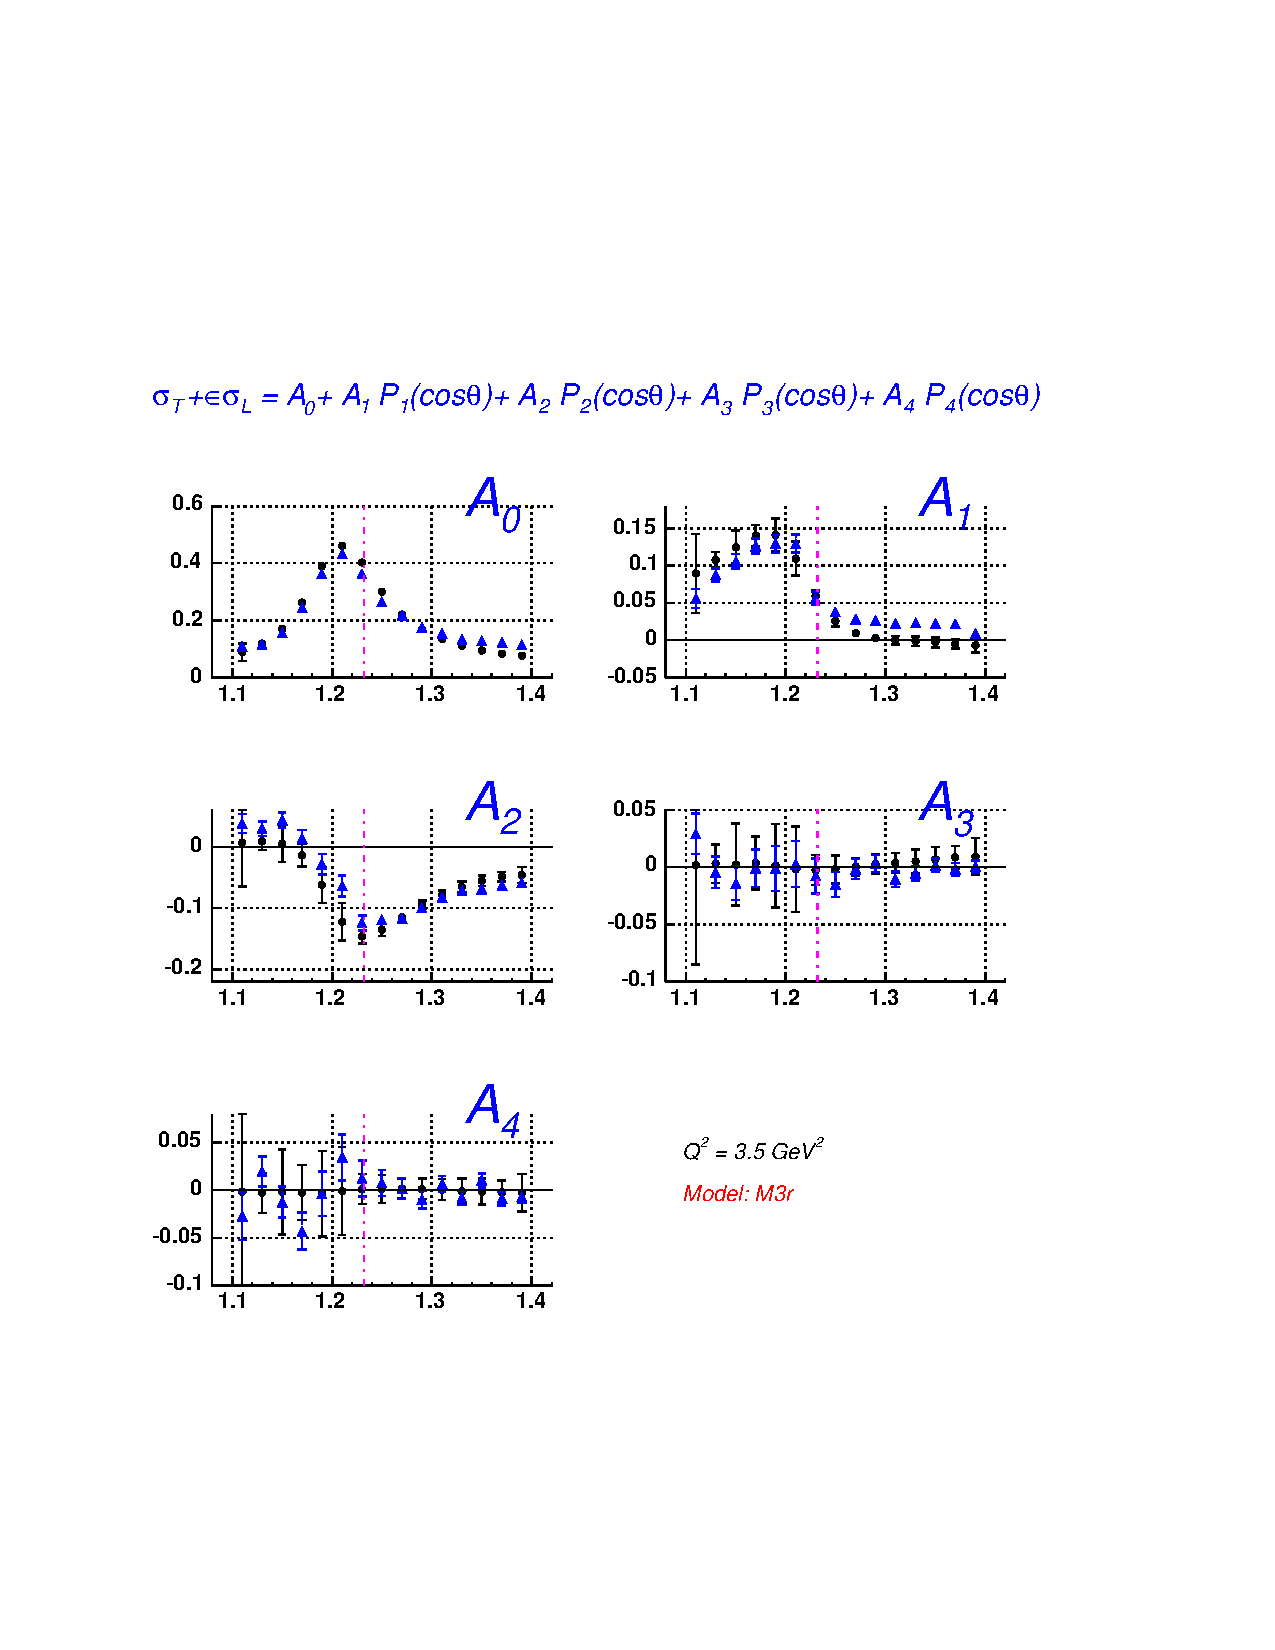
\includegraphics[width = 12cm, bb=30 130 540 700]{analysis/img/A_comp_m03r} 
  \caption[Coefficents of the Legendre expansion of $\sigma_T+\epsilon_L\sigma_L$ for the maid 2003 with Roper {\bf off} 
  generated cross 
  section  and experimental data ]
{ Coefficents of the Legendre expansion of $\sigma_T+\epsilon_L\sigma_L$ for the maid 2003 with Roper {\bf off}  generated cross 
  section (black) and experimental data (blue) }
 \label{fig:A_comp_m03r}
\end{center}
\end{figure}



% \cia
% \section{Discussion}
% The multipoles truncation fit result of $R_{EM}$ suggest a zero crossing between $Q^2$ of $3$ and $4.0$ GeV$^2$.
% This result for $R_{EM}$ would prove that the helicity is not conserved in this range of momentum transferred.
% A recent calculation of the non helicity conserving amplitude in the pQCD framework by Idilbi, 
% 
% The validity of the $M_{1+}$ dominance assumption is questionable, given the fact that the multipoles 
% coming from background and other resonances reach values up to $20-40\% $ of $|M_{1+}|$.
% 
% The result shown in \F{fig:JANRREMtrunc} also suggests that the multipole truncation might not
% be suited to extract the multipoles. 
% 
% The JANR fit  shows a constant negative value of around $-2.5\% $  with the point at $5$ $GeV^2$
% consistent with zero.
% 



%\cia
\section{Result for $G_M^*$ }
\label{sec:gmresult}






\begin{figure}[h]
 \begin{center}
 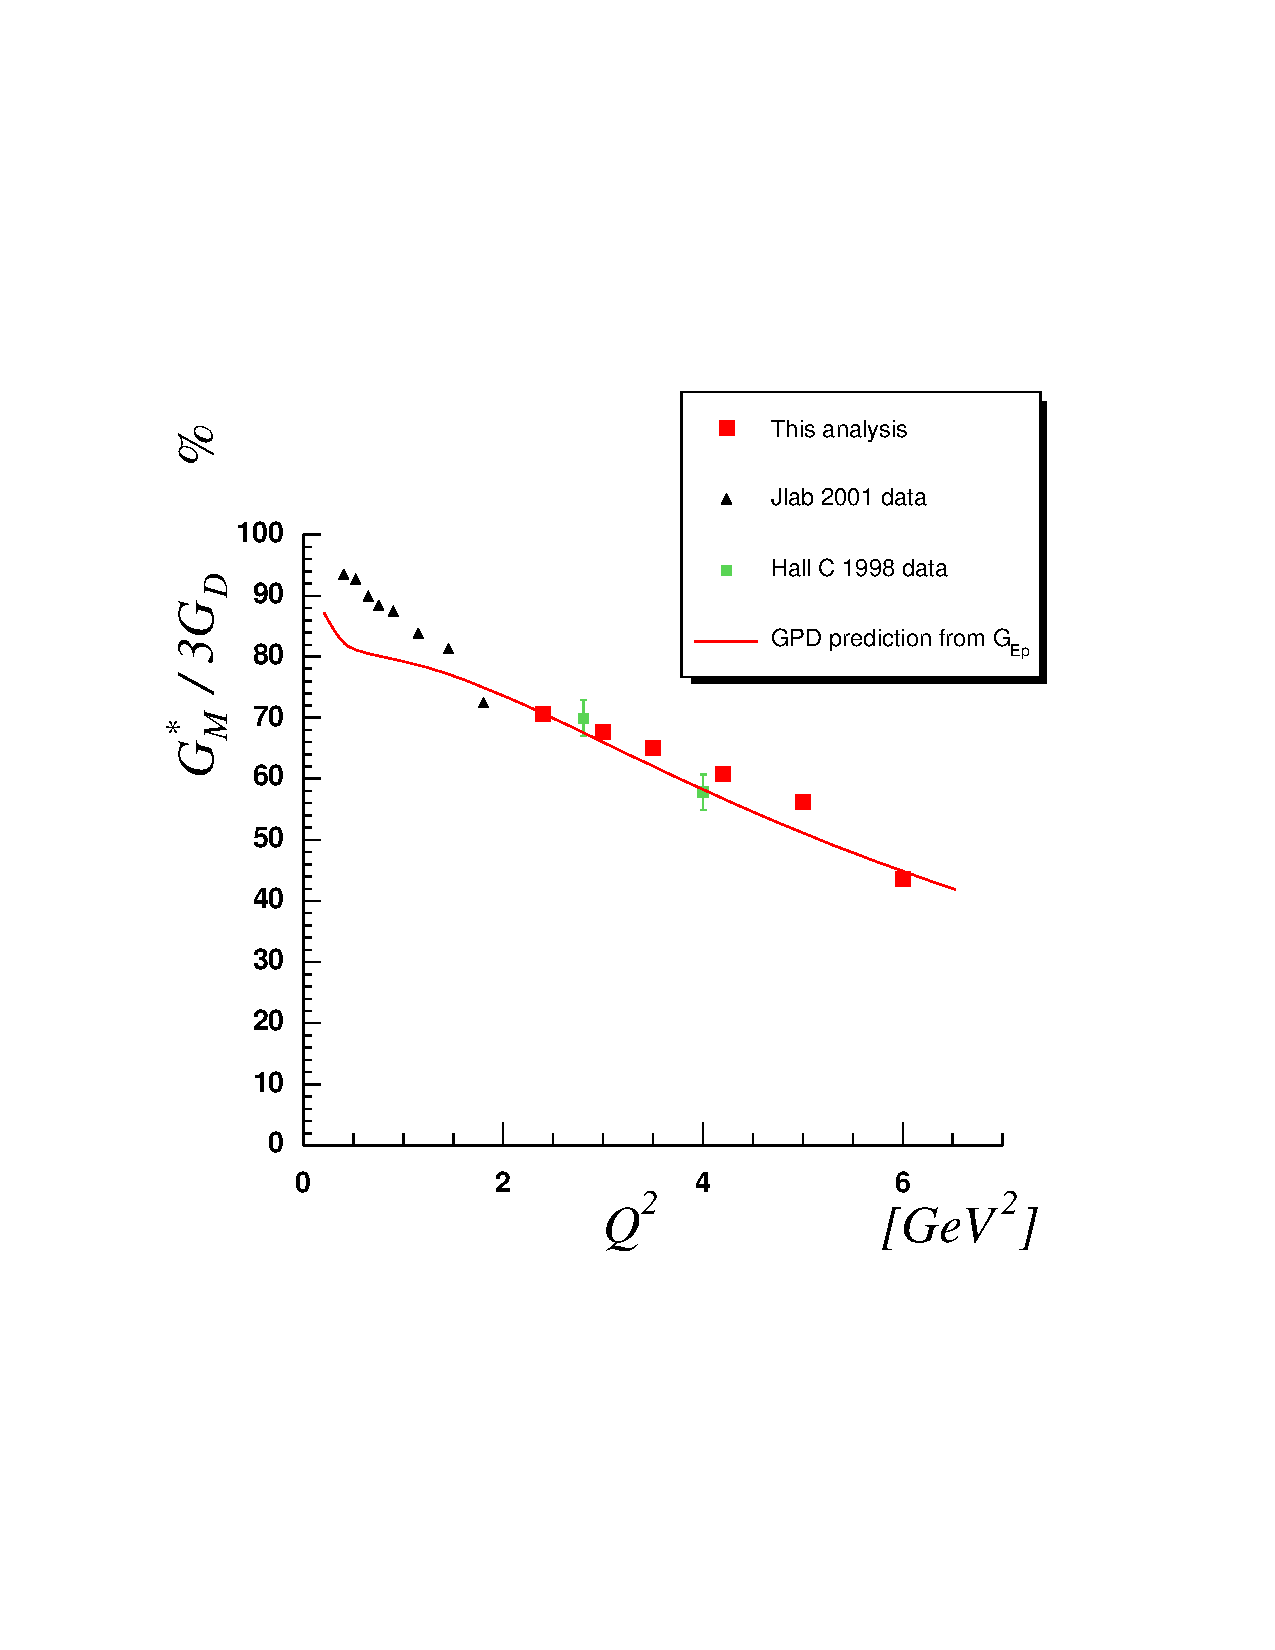
\includegraphics[width = 12cm, bb=30 130 520 600]{analysis/img/GMGDIP} 
  \caption[Result for $R_{SM}$ as a function of $Q^2$]
          {  Result for $G^*_M$ as a function of $Q^2$.}
 \label{fig:GMGDIP}
\end{center}
\end{figure}





\cia\vspace{-2 cm}
\section{Conclusions}
The differential cross section for the $\pi^0$ electroproduction in 
the $\Delta$ resonance has been measured in the $Q^2$ range $2$ to $6$ GeV$^2$
and $1.1 \le W \le 1.4$ GeV, with full coverage of the $\pi^0$ c.m. angles.
The structure functions $\sigma_T  + \epsilon_L \sigma_L$, $\sigma_{LT}$ and $\sigma_{TT}$ 
have been extracted using the $\phi^*$ dependance of the cross section.

Two calculations of the ratios  $R_{EM}$ and $R_{SM}$ have been presented.

A multipoles truncation fit of the data has been performed using the  $M_{1+}$ dominance and $\ell \le 2$
approximation.
This extraction of the ratio $R_{EM}$ suggest a zero crossing between $Q^2$ of $3$ and $4.0$ GeV$^2$,
while the ration $R_{SM}$ is about $-10\%$ and decreases with $Q^2$.
This result for $R_{EM}$ would prove that the helicity is not conserved in this range of momentum transferred.
The validity of the $M_{1+}$ dominance assumption is questionable, given the fact that the multipoles 
coming from background and other resonances reach values up to $20-40\% $ of $|M_{1+}|$.

A JANR fit that use the JLAB unitarian isobar model has been performed  for $Q^2$ up to $5$ $GeV^2$.
This extraction of the ratio $R_{EM}$ shows a constant negative value of around $-2.5\% $  with the point at $5$ $GeV^2$
consistent with zero.
The JANR fit suggest a smaller $M_{1-}$ amplitude when compared with the previous Hall-C data, suggesting 
that the $P_{11}$ signal is not as strong.















